
\documentclass[10pt]{article}
\usepackage[margin=0.78in]{geometry}
\usepackage{amsmath,amssymb,amsthm,mathtools}
\usepackage{booktabs,longtable,enumitem}
\usepackage{tikz}
\usepackage{graphicx}
\usetikzlibrary{arrows.meta,positioning,calc,shapes.geometric,fit,matrix}
\usepackage{xcolor}
\usepackage{hyperref}
\hypersetup{colorlinks=true,linkcolor=blue!50!black,citecolor=blue!50!black,urlcolor=blue!50!black}
\setlist[itemize]{leftmargin=1.4em,itemsep=2pt,topsep=2pt}
\setlist[enumerate]{leftmargin=1.5em,itemsep=2pt,topsep=2pt}
\newtheorem{theorem}{Theorem}[section]
\newtheorem{proposition}[theorem]{Proposition}
\newtheorem{lemma}[theorem]{Lemma}
\newtheorem{corollary}[theorem]{Corollary}
\newtheorem{definition}[theorem]{Definition}
\newtheorem{assumption}[theorem]{Assumption}
\newtheorem{example}[theorem]{Example}
\newtheorem{remark}[theorem]{Remark}
\newcommand{\RR}{\mathbb{R}}
\newcommand{\ZZ}{\mathbb{Z}}
\newcommand{\NN}{\mathbb{N}}
\newcommand{\CC}{\mathbb{C}}
\newcommand{\FF}{\mathbb{F}}
\newcommand{\PP}{\mathbb{P}}
\newcommand{\calX}{\mathcal{X}}
\newcommand{\calG}{\mathcal{G}}
\newcommand{\calK}{\mathcal{K}}
\newcommand{\calP}{\mathcal{P}}
\newcommand{\calM}{\mathcal{M}}
\newcommand{\calD}{\mathcal{D}}
\newcommand{\calC}{\mathcal{C}}
\newcommand{\calF}{\mathcal{F}}
\newcommand{\calO}{\mathcal{O}}
\newcommand{\bitsperbyte}{\operatorname{bits\text{-}per\text{-}byte}}
\newcommand{\Ent}{\operatorname{H}}
\newcommand{\KL}{\operatorname{KL}}
\newcommand{\Spec}{\operatorname{Spec}}
\newcommand{\Proj}{\operatorname{Proj}}
\newcommand{\Hom}{\operatorname{Hom}}
\newcommand{\Ext}{\operatorname{Ext}}
\newcommand{\Tor}{\operatorname{Tor}}
\newcommand{\im}{\operatorname{im}}
\newcommand{\rank}{\operatorname{rank}}
\newcommand{\cone}{\operatorname{Cone}}
\newcommand{\dist}{\operatorname{dist}}
\newcommand{\softmax}{\operatorname{softmax}}
\newcommand{\argmax}{\operatorname*{arg\,max}}
\newcommand{\loss}{\mathcal{L}}
\newcommand{\eps}{\varepsilon}
\numberwithin{equation}{section}
\definecolor{darkblue}{RGB}{28,74,126}
\definecolor{darkgreen}{RGB}{20,112,80}
\definecolor{darkred}{RGB}{143,45,45}
\definecolor{softgray}{RGB}{245,247,250}
\sloppy
\begin{document}

\begin{titlepage}
\centering
{\Huge\bfseries ToricGT II: Dynamical, Ergodic, and Derived Persistence Geometry for Iterative Reasoning Agents\par}
\vspace{8pt}
{\Large A second-iteration NeurIPS-style research article and objective catalogue for bits-per-byte-safe ToricGT training\par}
\vspace{16pt}
{\large Amelie Schreiber}\par
{\large June 2026}\par
\vfill
\begin{abstract}
ToricGT I used toric charts, tropical attention, GraphCG concept axes, noncommutative-torus phase channels, GFlowNet graph-of-thought search, and finite BGG/Koszul certificates to regularize graph-token reasoning under a strict bits-per-byte compression contract \cite{toricgt1}. ToricGT II extends that program from isolated certificates to a dynamical theory of reasoning trajectories. A reasoning step is modeled as a standardized padded packet of embeddings, graph tokens, verifier fields, behavior-corridor coordinates, and output-token context. From each packet we build filtered directed simplicial complexes, multigraded persistence modules, coherent sheaf data, and derived objects. The learned graph-to-graph map then induces a dynamical system on packets, a functorial evolution of persistence modules, a derived endomorphism up to measured cone error, and a symbolic toric process inside a fan-decomposed embedding space. The central compression principle is conditional mutual information: a certificate helps bits-per-byte only when it is prefix-visible and lowers the conditional entropy of future bytes enough to justify its artifact and runtime cost. The central reasoning principle is functorial stability: local reasoning moves should preserve homology, filtrations, Cox degrees, bundle transition data, tableaux weights, and behavior-corridor constraints up to quantified residuals. We prove compactness, stability, invariant-measure, ergodic-average, entropy-rate, finite-generation, chain-map, sheaf-gluing, and toric symbolic-dynamics theorems under explicit finite-state or Lipschitz assumptions. We then reselect the best 20 objectives from the previous ToricGT toric-objective catalogue and rewrite them for the new dynamical persistence setting. Finally, we add 20 new objectives designed specifically for iterative reasoning trajectories, derived persistence modules, ergodic toric dynamics, representation-theoretic combinatorics, tone/personality control, accuracy, and bits-per-byte-safe deployment.
\end{abstract}
\vfill
\begin{minipage}{0.9\textwidth}
\textbf{Design contract.} Toric geometry is used here as a compression and control instrument, not as decoration. Cones, one-dimensional cones, affine semigroups, normal fans, Cox coordinates, sheaves, vector bundles, differential forms, Cech complexes, local cohomology, Chow/Stanley-Reisner rings, secondary fans, and Gale duality are converted into finite certificates, low-rank probes, and audit metrics; the toric vocabulary follows the standard constructions in \cite{cls}. Any objective may remain in the teacher or analysis stack, but it enters the deployable student only after score-first bits-per-byte evaluation, quantized round-trip export, artifact-byte accounting, and matched ablations.
\end{minipage}
\end{titlepage}
\tableofcontents
\clearpage

\section{Purpose, scope, and contributions}
ToricGT II begins from a specific modeling problem. Modern reasoning agents do not merely map a prompt to an answer. They execute a sequence of hidden steps: retrieving evidence, decomposing a problem, selecting a local proof route, deciding how much uncertainty to expose, controlling output tone, formatting an answer, and sometimes branching and merging graph-of-thought alternatives. ToricGT I already represented many of these objects as graph tokens and finite algebraic certificates. The missing piece was a dynamical theory of the objects produced at each reasoning step and the objects obtained by repeated application of the learned graph-to-graph map.

This article supplies that theory. The guiding object is a standardized reasoning step $x_t\in \calX$. It is a padded packet containing hidden vectors, token masks, graph edges, certificate fields, behavior-corridor coordinates, verifier fields, and a strict-prefix byte context. From $x_t$ we construct a filtered simplicial object $\calK(x_t)$, a multigraded persistence module $\calM(x_t)$, a complex in a derived category $\calD(x_t)$, a sheaf or vector-bundle chart object $\calF(x_t)$, and a toric chart code $\tau(x_t)$. The model supplies a map
\begin{equation}
T_\theta:\calX\to\calX,\qquad x_{t+1}=T_\theta(x_t),
\end{equation}
or, under sampling, a Markov kernel $P_\theta(x,dy)$. The research question becomes: what structural properties of the induced sequence
\begin{equation}
\bigl(x_t,\calK_t,\calM_t,\calD_t,\calF_t,\tau_t\bigr)_{t\ge 0}
\end{equation}
make future bytes more predictable, answers more accurate, and behavior more controllable?

The answer is not ``more structure'' in the abstract. The answer is structure that lowers conditional entropy and survives deployment. The most important identity in the paper is the bits-per-byte side-information identity: if a prefix-visible certificate $Z_t$ is actually useful for predicting the next byte $B_t$, then an optimal predictor improves expected log loss by $I(B_t;Z_t\mid \mathcal{F}_t)$ bits. If $Z_t$ is decorative, the mutual information is zero. If $Z_t$ is expensive, its artifact cost may dominate. If $Z_t$ depends on future validation bytes, the score is invalid. The same rule governs every objective below.

\paragraph{Main contributions.}
\begin{enumerate}
\item We define standardized reasoning-step packets and construct filtered directed simplicial complexes from their token, evidence, verifier, tone, style, and memory coordinates.
\item We develop a dynamical theory of iterative reasoning: deterministic maps and Markov kernels on compact packet spaces, induced evolution of complexes, persistence modules, sheaves, and derived objects.
\item We prove stability and functoriality results showing when learned graph-to-graph maps produce valid persistence-module morphisms and when residuals are exactly measured by mapping cones.
\item We connect ergodic theory to bits-per-byte: time-averaged bits-per-byte, Betti drift, certificate entropy, behavior-corridor cost, and verifier accuracy converge to invariant-measure expectations under standard assumptions.
\item We describe algebraic geometry inside toric embedding spaces, using one-dimensional cones, normal fans, Cox degrees, support functions, differential forms, canonical sheaves, and Cech gluing to make reasoning states auditable.
\item We integrate representation theory and Young-tableau combinatorics through Weyl chambers, crystals, Schur functors, Littlewood-Richardson certificates, and tableau normal forms.
\item We deliver a 40-objective catalogue: 20 reselected ToricGT objectives rewritten for dynamic persistence and 20 new objectives designed from the start for iterative reasoning, ergodic dynamics, derived persistence, bits-per-byte, tone/personality corridors, and accuracy.
\end{enumerate}


\begin{figure}[!htbp]
\centering
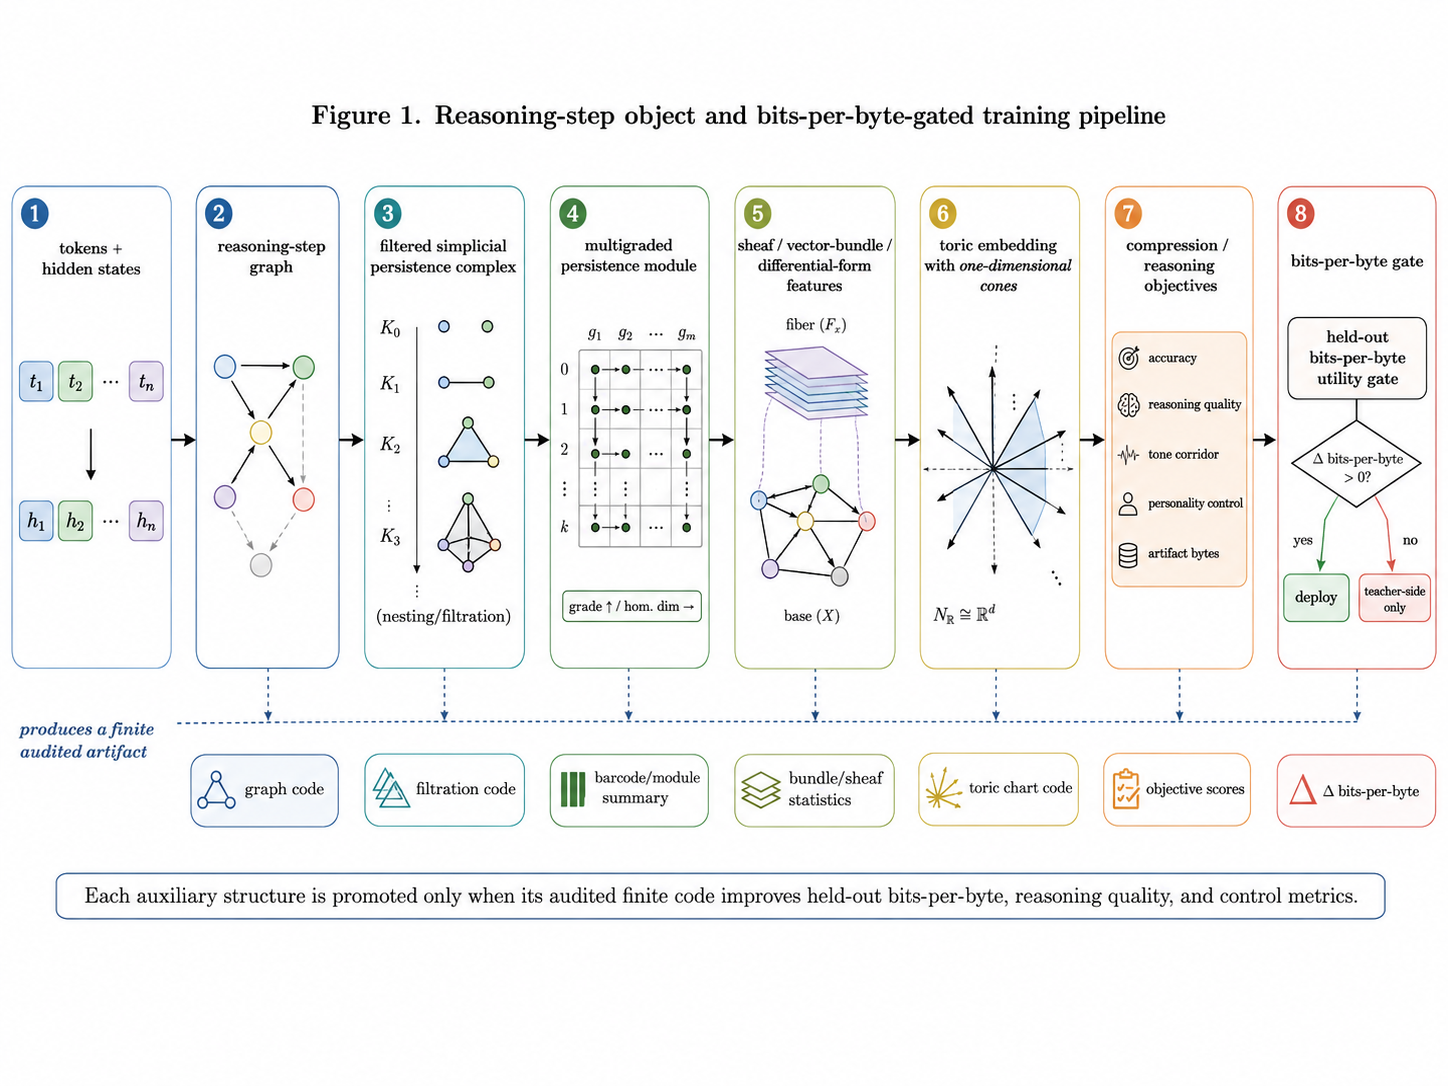
\includegraphics[width=\textwidth]{neurips_style_reasoning_pipeline_diagram.png}
\caption{Reasoning-step object and bits-per-byte-gated training pipeline. A standardized step is converted into graph, persistence, sheaf/vector-bundle, differential-form, toric-chart, objective, and gate artifacts. The finite audit row emphasizes that structure is retained only when it improves held-out bits-per-byte, reasoning quality, and control metrics.}
\label{fig:reasoning-step-pipeline}
\end{figure}

\section{Toric and ToricGT background}
\subsection{Toric language used by the paper}
Let $N\simeq\ZZ^n$ be a lattice, let $M=\Hom(N,\ZZ)$, and write $\langle m,u\rangle$ for the pairing, following the character/cocharacter convention of toric geometry \cite{cls}. A rational polyhedral cone $\sigma\subset N_\RR$ is a cone generated by finitely many lattice vectors. Its dual is
\begin{equation}
\sigma^\vee=\{m\in M_\RR:\langle m,u\rangle\ge 0\;\forall u\in\sigma\}.
\end{equation}
The affine semigroup of $\sigma$ is $S_\sigma=\sigma^\vee\cap M$, and the corresponding normal affine toric variety is
\begin{equation}
U_\sigma=\Spec\CC[S_\sigma].
\end{equation}
A one-dimensional cone $\rho\subset \sigma$ has a primitive generator $u_\rho\in \rho\cap N$. ToricGT II uses one-dimensional cones as coordinate axes for sparse certificates: Cox variables, divisors, residues, behavior faces, and local obstruction terms are indexed by such cones.

A fan $\Sigma$ is a finite set of strongly convex rational polyhedral cones closed under faces and compatible intersections. The toric variety $X_\Sigma$ is glued from the affine charts $U_\sigma$ for $\sigma\in\Sigma$. A lattice polytope $P\subset M_\RR$ gives a normal fan $\Sigma_P$; for a face $Q\preceq P$, the cone $\sigma_Q$ is generated by primitive inward normal vectors of facets containing $Q$. This face-cone dictionary is the origin of ToricGT's active-face code: a hidden max-plus or ReLU decision exposes a face of a Newton polytope, hence selects a cone of a normal fan.

The Cox ring of a toric variety is a multigraded polynomial ring with one variable $x_\rho$ for each one-dimensional cone $\rho\in\Sigma(1)$. The grading is by the divisor class group. An irrelevant ideal cuts out invalid coordinate regions. In ToricGT II, Cox degrees become a low-cost way to audit whether a reasoning trajectory preserves evidence type, proof obligation, verifier status, output tone, and safety/refusal mode.

Sheaves enter because reasoning is local-to-global. A coherent sheaf $\calF$ assigns modules of sections to open sets; a vector bundle is equivalently a locally free sheaf; a toric divisor $D$ gives $\calO_X(D)$; Cech complexes compute cohomology from affine covers; differential forms and the cotangent sheaf measure infinitesimal changes in a chart \cite{cls,hartshorne}. These notions become trainable certificates: local reasoning windows should glue, transition functions should satisfy cocycles, and differential-form residues should control boundary behavior along tone, refusal, and evidence divisors.

\subsection{ToricGT I recap}
ToricGT I represented structured reasoning problems as typed graph tokens, processed them by token-permutation-equivariant Transformer blocks, and attached optional toric, tropical, GraphCG, GFlowNet, noncommutative-torus, and BGG/Koszul probes. The operational principle was finite certification. A minibatch could carry a sign-vector poset, a sparse chain complex, a Betti profile, a Gale-dual label, an Euler-Koszul complex, a normal-fan active face, or a behavior-corridor certificate. The model was trained to align hidden trajectories with these finite objects, while the compressed bits-per-byte-facing student retained only components that improved validation log score under artifact limits.

ToricGT II preserves that discipline but changes the object of study. Instead of asking whether one hidden state satisfies one certificate, we ask whether a whole iterative reasoning trajectory has stable dynamical, topological, algebraic, derived, toric, and behavior-corridor invariants.

\section{Reasoning steps as compact dynamical states}
\begin{definition}[Standardized reasoning step]
Fix integers $n_\star,m_\star,d$ and finite type sets for tokens, edges, and certificate fields. A standardized reasoning step is a tuple
\begin{equation}
x=(H,A,E,\mu,\xi,c,v,r,b_{<t}),
\end{equation}
where $H\in[-R,R]^{n_\star\times d}$ is a padded hidden table, $A\in\{0,1\}^{n_\star\times n_\star}$ is a padded relation mask, $E$ stores typed edge attributes, $\mu$ stores token-validity and certificate-validity masks, $\xi=B^\top H$ are GraphCG concept/behavior coordinates, $c$ is a toric chart code, $v$ is a verifier/evidence vector, $r$ is a retrieval-memory signature, and $b_{<t}$ is the strict-prefix byte context available at the step. The bounded packet space is denoted $\calX$.
\end{definition}

The padding convention is practical. A reasoning step may be a full natural-language thought, a graph-of-thought vertex, a proof subroutine, or a chunk of model computation. Padding fixes the number of vectors and tokens so that topology and algebra can be computed from a stable tensor shape. The semantic boundary is flexible; the mathematical object is the standardized packet.

\begin{assumption}[Score-first measurability]
At validation step $t$, every component of $x_t$ used to predict $b_t$ is measurable with respect to the sigma-field generated by fixed model parameters, public metadata, internal randomness sampled before seeing $b_t$, and the strict prefix $b_{<t}$. Updates using $b_t$ occur only after the log score for $b_t$ is recorded.
\end{assumption}

\begin{proposition}[Compact packet space]
For fixed padding sizes, bounded real fields, finite masks, finite types, and finite certificate vocabularies, $\calX$ is a compact metric space.
\end{proposition}
\begin{proof}
The real-valued fields lie in finite products of compact intervals. The masks, type labels, and finite certificate ids lie in finite discrete spaces, hence compact. A finite product of compact spaces is compact. A metric is obtained by adding Euclidean distances for real fields and Hamming distances for discrete fields.
\end{proof}

\begin{definition}[Learned reasoning dynamics]
A deterministic ToricGT II reasoning model is a measurable map $T_\theta:\calX\to\calX$. If all active masks and routing choices are fixed on a cell, $T_\theta$ is continuous on that cell. A stochastic model is a Markov kernel $P_\theta(x,dy)$ obtained by sampling GFlowNet actions, retrieval candidates, dropout-like internal choices, or decoding branches before reading the next validation byte.
\end{definition}

\begin{theorem}[Existence of invariant reasoning measures]
If $\calX$ is compact and $T_\theta:\calX\to\calX$ is continuous, then there exists a $T_\theta$-invariant Borel probability measure. If $P_\theta$ is a Feller Markov kernel on $\calX$, then there exists a stationary probability measure.
\end{theorem}
\begin{proof}
For the deterministic case, fix any probability measure $\nu$ and form the Cesaro averages $\nu_T=T^{-1}\sum_{t=0}^{T-1}(T_\theta^t)_\#\nu$. The space of probability measures on compact $\calX$ is weakly compact, so a subsequence converges to some $\mu$. Continuity of $T_\theta$ implies $(T_\theta)_\#\mu=\mu$ by the standard Krylov-Bogolyubov argument. The Feller-kernel case is identical with pushforward replaced by the Markov operator on probability measures.
\end{proof}


\begin{figure}[!htbp]
\centering
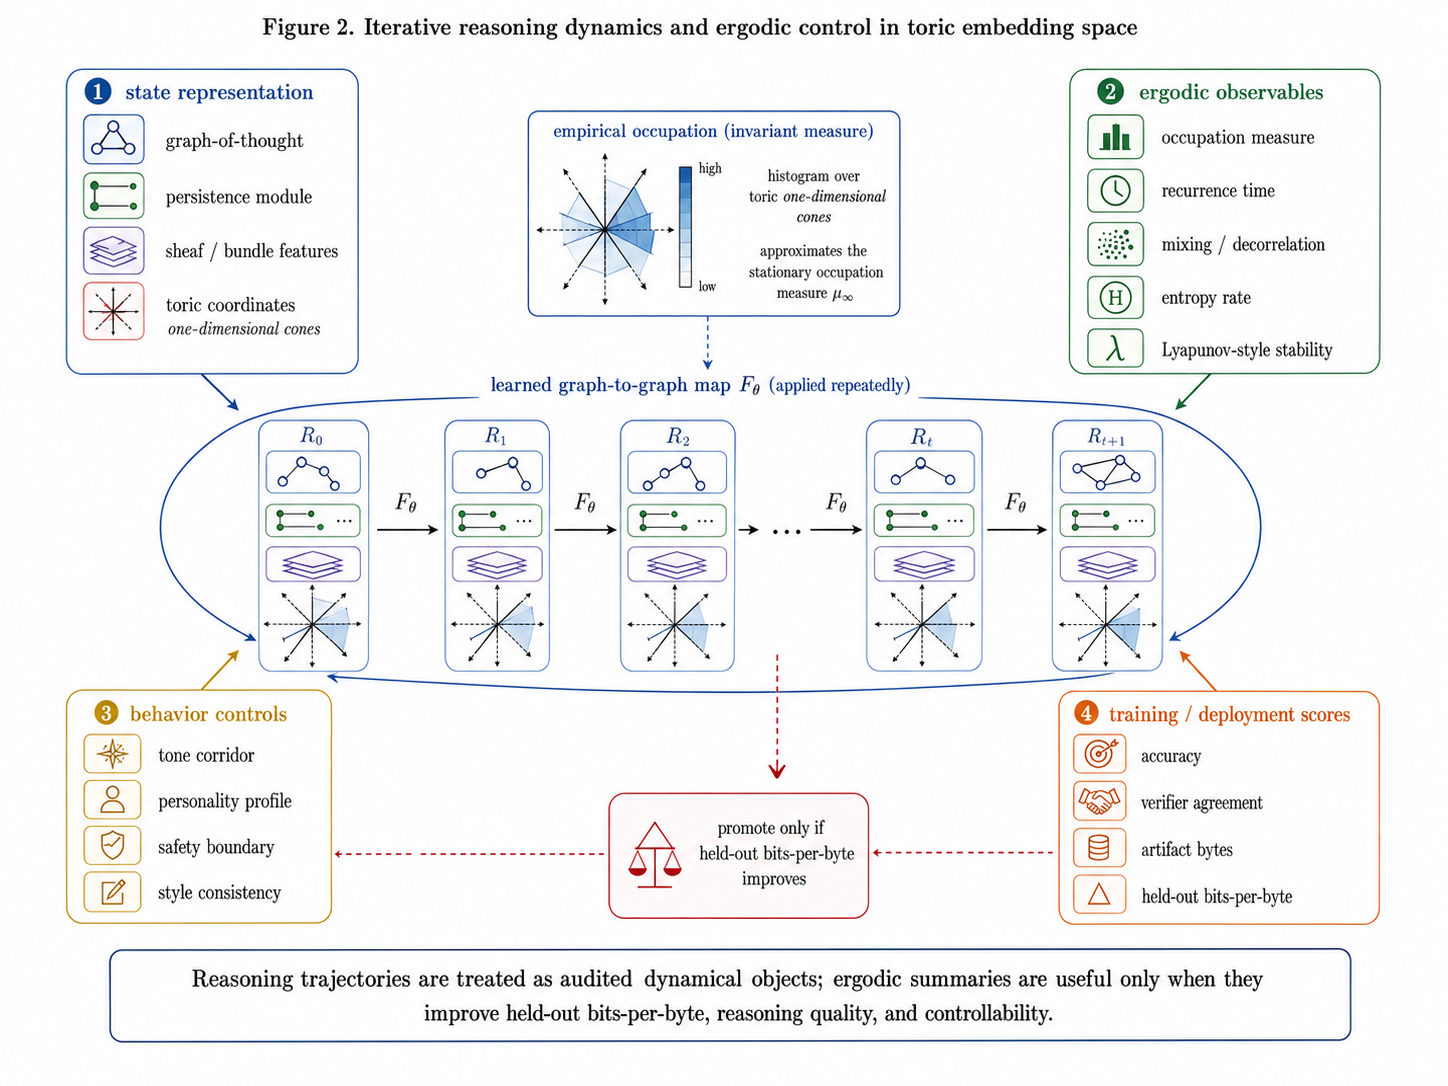
\includegraphics[width=\textwidth]{iterative_reasoning_and_control_dynamics.png}
\caption{Iterative reasoning dynamics and ergodic control in toric embedding space. The repeated learned graph-to-graph map evolves graph-of-thought, persistence, sheaf/bundle, and toric-coordinate state. Ergodic observables, behavior controls, and deployment scores are promoted only when held-out bits-per-byte improves.}
\label{fig:iterative-reasoning-ergodic-control}
\end{figure}

\section{Filtered complexes attached to a reasoning step}
\subsection{Undirected, directed, and behavior-aware complexes}
Let $z_i=B^\top h_i\in\RR^r$ be the GraphCG coordinate of token or factor $i$ in a step. We use a weighted distance
\begin{equation}
d_x(i,j)=\|W(z_i-z_j)\|_2+\lambda_e |e_i-e_j|+\lambda_v |v_i-v_j|+\lambda_c\,\mathbf{1}\{c_i\ne c_j\}.
\end{equation}
An antisymmetric score $\Omega_x(i,j)=-\Omega_x(j,i)$ records directed evidence flow, retrieval precedence, proof dependency, or phase orientation. For thresholds $\alpha=(\rho,\eta,\kappa)$, where $\rho$ controls distance, $\eta$ controls evidence compatibility, and $\kappa$ controls behavior-corridor compatibility, define a directed edge $i\to j$ to be admissible when
\begin{equation}
d_x(i,j)\le \rho,
\qquad
\mathrm{evidence}(i,j)\ge \eta,
\qquad
\mathrm{corridor}(i,j)\le \kappa,
\qquad
\Omega_x(i,j)\ge 0.
\end{equation}

\begin{definition}[Directed filtered flag complex]
For a threshold $\alpha$, $\calK_\alpha^\to(x)$ is the directed flag complex whose ordered $p$-simplices $(i_0,\ldots,i_p)$ satisfy $i_a\to i_b$ for every $a<b$. If $\alpha\le \beta$ coordinatewise and admissibility is monotone, then $\calK_\alpha^\to(x)\subseteq \calK_\beta^\to(x)$. The family $\calK_\bullet^\to(x)$ is the filtered directed reasoning complex of $x$.
\end{definition}

The undirected version is the ordinary flag complex obtained by ignoring $\Omega_x$. The behavior-aware version keeps $\Omega_x$ and tags simplices by purpose: evidence, plan, verifier, style, memory, refusal, or answer commitment. A good reasoning step should have enough topology to represent dependency, but not so much topology that all factors coactivate indiscriminately.

\begin{definition}[Multifiltration index poset]
Let $P=\NN^s$ or a finite grid $P=\prod_{a=1}^s\{0,\ldots,L_a\}$. A multifiltration is a functor
\begin{equation}
\calK_x:P\to \mathbf{Simp},\qquad \alpha\mapsto \calK_\alpha(x),
\end{equation}
where $\alpha\le\beta$ gives an inclusion $\calK_\alpha(x)\hookrightarrow\calK_\beta(x)$. Typical coordinates are radius, evidence threshold, verifier threshold, style distance, Cox degree, active fan margin, and time-within-step.
\end{definition}

\begin{definition}[Persistence module of a reasoning step]
For a field $\FF$, define
\begin{equation}
\calM_p(x)(\alpha)=H_p(\calK_\alpha(x);\FF),
\end{equation}
with structure maps induced by inclusions. This is a persistence module over $P$. When $P=\NN^s$, it is equivalently an $\NN^s$-graded module over $S=\FF[u_1,\ldots,u_s]$ under the usual correspondence between multigraded modules and functors from $\NN^s$.
\end{definition}


\begin{figure}[!htbp]
\centering
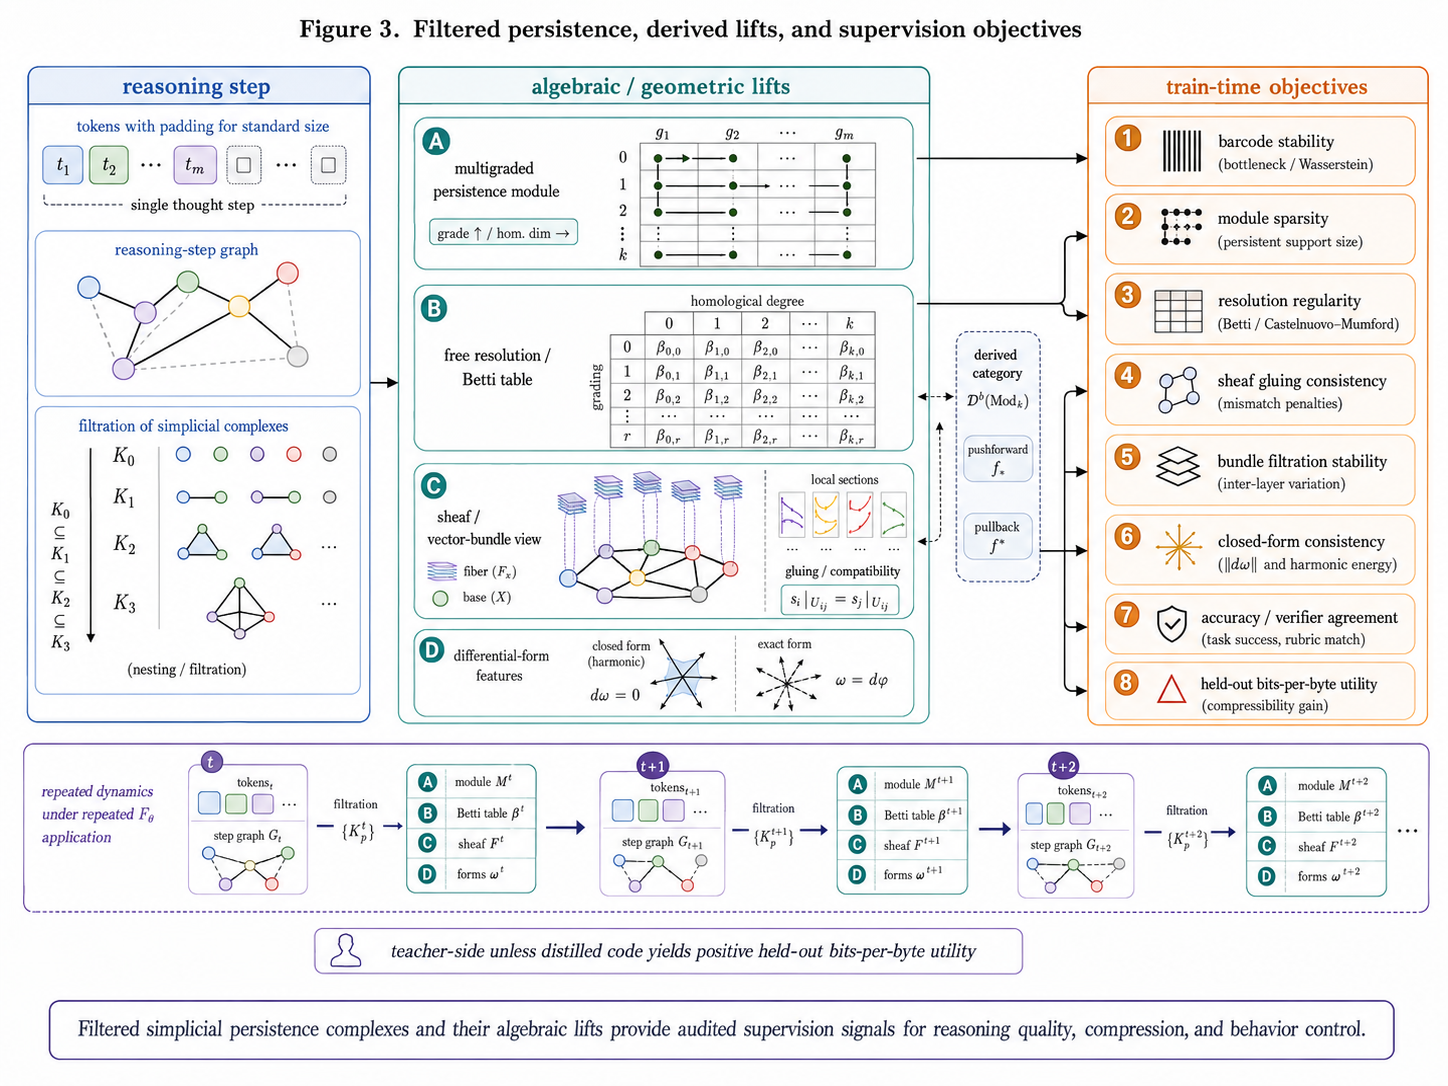
\includegraphics[width=\textwidth]{filtered_persistence_and_algebraic_supervision.png}
\caption{Filtered persistence, derived lifts, and supervision objectives for a standardized reasoning step. The diagram shows the construction of filtered simplicial complexes, multigraded persistence modules, free resolutions, sheaf/vector-bundle views, differential-form features, derived-category lifts, and their train-time losses, with held-out bits-per-byte as the deployment utility.}
\label{fig:filtered-persistence-derived-lifts}
\end{figure}

\subsection{Stability of step complexes}
\begin{theorem}[One-step persistence stability]
Let $x,y\in\calX$ have the same valid-token mask and let $d_x,d_y$ be their symmetric distance matrices. For Vietoris-flag filtrations, the degree-$p$ persistence diagrams satisfy
\begin{equation}
d_B(D_p(x),D_p(y))\le \|d_x-d_y\|_\infty.
\end{equation}
If $d_x$ is $L_d$-Lipschitz as a function of the hidden table, then
\begin{equation}
d_B(D_p(x),D_p(y))\le L_d\|H_x-H_y\|_\infty.
\end{equation}
\end{theorem}
\begin{proof}
If $\|d_x-d_y\|_\infty\le \eps$, every edge present at radius $\rho$ in the filtration of $x$ is present at radius $\rho+\eps$ in the filtration of $y$, and conversely. Hence the filtrations are $\eps$-interleaved. The algebraic stability theorem for persistence gives the bottleneck bound. The second inequality follows by Lipschitz continuity of $d_x$ in the hidden table.
\end{proof}

This theorem is the first reason filtered complexes are useful for training. A small perturbation of a hidden step cannot arbitrarily change long-lived topology. Therefore persistence losses measure stable structure rather than noise, provided the model is trained away from zero-margin topological decisions.

\section{Dynamics of persistence modules and derived objects}
\subsection{Model-induced maps}
The learned map $T_\theta$ does not automatically define a simplicial map $\calK_\alpha(x)\to\calK_\beta(T_\theta x)$. ToricGT II therefore learns or audits a transport matrix $P_x\in[0,1]^{n_\star\times n_\star}$, usually a row-stochastic nearest-neighbor or attention transport, and accepts it as a chain-level map only when it sends vertices, edges, and triangles to valid target simplices after a small filtration shift.

\begin{definition}[Filtered step morphism]
A filtered step morphism from $x$ to $y$ consists of a monotone index map $s:P\to P$, chain maps
\begin{equation}
F_{p,\alpha}:C_p(\calK_\alpha(x))\to C_p(\calK_{s(\alpha)}(y))
\end{equation}
for all $p,\alpha$, and commutative squares with the inclusion maps. The chain residual is
\begin{equation}
\mathrm{Res}_{\partial}(F)=\sum_{p,\alpha}\|\partial_y F_{p,\alpha}-F_{p-1,\alpha}\partial_x\|_F^2.
\end{equation}
\end{definition}

\begin{proposition}[Filtered chain maps induce persistence-module morphisms]
If $\mathrm{Res}_{\partial}(F)=0$ and the squares with filtration inclusions commute, then $F$ induces a morphism of persistence modules
\begin{equation}
H_p(\calK_\bullet(x))\longrightarrow H_p(\calK_{s(\bullet)}(y)).
\end{equation}
\end{proposition}
\begin{proof}
The chain-map identity sends cycles to cycles and boundaries to boundaries, hence induces maps on homology at each filtration index. Commutativity with inclusions makes these homology maps natural in the index poset, which is exactly a persistence-module morphism.
\end{proof}

\begin{definition}[Derived reasoning object]
Let $S=\FF[u_1,\ldots,u_s]$. The degree-$p$ multigraded persistence module $\calM_p(x)$ has a finite free resolution on finite training grids,
\begin{equation}
F_\bullet(x):\quad 0\to F_r\to\cdots\to F_0\to \calM_p(x)\to 0.
\end{equation}
The derived reasoning object is the quasi-isomorphism class of $F_\bullet(x)$ in $D^b(\mathrm{gr}\text{-}S)$, optionally enriched with Cox degrees, sheaf labels, behavior-corridor labels, and representation-theoretic weights.
\end{definition}

\begin{theorem}[Finite-grid persistence modules are finitely generated]
Let $P=\prod_{a=1}^s\{0,\ldots,L_a\}$ and suppose every $\calK_\alpha(x)$ has at most $n_\star$ vertices. Extend $\calM_p(x)$ to an $\NN^s$-module by keeping it constant after the grid boundary. Then $\calM_p(x)$ is a finitely generated multigraded $S$-module.
\end{theorem}
\begin{proof}
There are finitely many grid indices and each vector space $H_p(\calK_\alpha(x);\FF)$ is finite-dimensional because the complex has finitely many simplices. Choose a basis for each grid vector space and lift each basis element to a generator in its multidegree. The $S$-action propagates generators forward along the coordinate directions; after the grid boundary the module is constant, so no new generators are needed. Hence finitely many homogeneous generators suffice.
\end{proof}

\begin{theorem}[Mapping-cone residual measures derived failure]
Let $F_\bullet:C_\bullet\to D_\bullet$ be a degree-zero map of finite chain complexes. If $F_\bullet$ is a chain map, its mapping cone $\mathrm{Cone}(F)$ is a complex and fits into a distinguished triangle
\begin{equation}
C_\bullet\xrightarrow{F}D_\bullet\to \mathrm{Cone}(F)\to C_\bullet[1]
\end{equation}
in the derived category. If $F_\bullet$ is not a chain map, the obstruction is exactly the graded commutator $\partial_DF-F\partial_C$.
\end{theorem}
\begin{proof}
For a chain map, the usual cone differential $\delta(d,c)=(\partial_Dd+F c,-\partial_C c)$ squares to zero precisely because $\partial_D^2=\partial_C^2=0$ and $\partial_DF=F\partial_C$. The standard cone construction gives the distinguished triangle. Conversely, computing $\delta^2(d,c)$ leaves the term $(\partial_DF-F\partial_C)c$, so the failure of the cone to be a complex is exactly the commutator.
\end{proof}

This theorem turns a high-level phrase - ``the model should respect derived structure'' - into a concrete loss: penalize the commutator and the homology of the cone when the transition should be an equivalence.

\section{Ergodic theory of iterative reasoning}
\subsection{Observables and invariant averages}
Let $\varphi:\calX\to\RR$ be any bounded measurable observable: local bits-per-byte, verifier error, behavior-corridor distance, Betti drift, Cox-degree violation, Cech obstruction, tableau inversion count, or fan-cell entropy.

\begin{theorem}[Birkhoff averages for reasoning observables]
Let $\mu$ be an invariant probability measure for $T_\theta$ and let $\varphi\in L^1(\mu)$. Then
\begin{equation}
\bar\varphi_T(x)=\frac1T\sum_{t=0}^{T-1}\varphi(T_\theta^t x)
\end{equation}
converges for $\mu$-almost every $x$ to a $T_\theta$-invariant function $\bar\varphi(x)$. If $\mu$ is ergodic, then $\bar\varphi(x)=\int \varphi\,d\mu$ almost surely.
\end{theorem}
\begin{proof}
This is Birkhoff's ergodic theorem applied to the measure-preserving system $(\calX,\mu,T_\theta)$.
\end{proof}

In practice, this theorem justifies reporting long-run averages of structure metrics rather than cherry-picking steps. If a model has low average bits-per-byte but periodically enters high-risk behavior strata, the observable for corridor violation exposes that regime. If a model has good local proofs but high Betti drift, the topological observable exposes unstable planning.

\begin{definition}[Toric symbolic process]
Let $\Pi=\{C_1,\ldots,C_R\}$ be a finite partition of $\calX$ by toric fan cells, active faces, Cox-degree bins, behavior alcoves, or tableau/crystal labels. The symbolic process of a trajectory is
\begin{equation}
s_t=i\quad\Longleftrightarrow\quad x_t\in C_i.
\end{equation}
Its empirical transition matrix is $\widehat P_{ij}=\#\{t:s_t=i,s_{t+1}=j\}/\#\{t:s_t=i\}$.
\end{definition}

\begin{theorem}[Entropy-rate upper bound from a toric transition graph]
Suppose the symbolic process is supported on a directed graph $G_\Pi$ with adjacency matrix $A_\Pi$. Then the topological entropy of the symbolic process is at most $\log \lambda_{\max}(A_\Pi)$. If the process is stationary Markov with transition matrix $P$, its Shannon entropy rate is
\begin{equation}
h(P)=-\sum_i \pi_i\sum_j P_{ij}\log_2 P_{ij},
\end{equation}
where $\pi$ is stationary.
\end{theorem}
\begin{proof}
The number of length-$T$ admissible paths in the graph is at most $\mathbf{1}^\top A_\Pi^{T-1}\mathbf{1}$, whose exponential growth rate is bounded by the spectral radius. The Markov entropy-rate formula is standard and follows from stationarity and conditional entropy $H(s_{t+1}\mid s_t)$.
\end{proof}

A lower transition entropy is not automatically better. It is better only when verifier accuracy and answer diversity remain high. The desired regime is low entropy of irrelevant hidden variations and high entropy only where multiple valid reasoning routes or answer styles are genuinely needed.

\subsection{Bits-per-byte as conditional entropy reduction}
\begin{theorem}[Prefix-visible certificates improve optimal bits-per-byte by mutual information]
Let $\mathcal{F}_t$ be the strict-prefix sigma-field and let $Z_t$ be a certificate measurable with respect to $\mathcal{F}_t$. Let $B_t$ be the next byte. The optimal expected log-loss improvement, in bits, from using $Z_t$ in addition to $\mathcal{F}_t$ is
\begin{equation}
\Ent(B_t\mid \mathcal{F}_t)-\Ent(B_t\mid \mathcal{F}_t,Z_t)=I(B_t;Z_t\mid \mathcal{F}_t).
\end{equation}
Consequently, a certificate family can reduce expected bits-per-byte only through conditional information about future bytes that is already available before the score is recorded.
\end{theorem}
\begin{proof}
The optimal log-loss predictor under a sigma-field is the true conditional distribution. Its expected base-two log loss equals the corresponding conditional entropy. Subtracting the two optimal losses gives the conditional mutual information identity.
\end{proof}

This theorem is the compression center of ToricGT II. Persistence diagrams, Betti tables, normal-fan cells, bundle cocycles, differential-form residues, or Young tableaux are useful only when they become compact prefix-visible summaries that change the next-byte distribution in the correct direction.

\begin{definition}[Net structural compression utility]
For a certificate family $Z$ with per-token runtime cost $c_{\rm run}$ and serialized artifact cost $c_{\rm art}$, define
\begin{equation}
U_{\rm net}(Z)=\widehat I(B_t;Z_t\mid\mathcal F_t)-\lambda_{\rm run}c_{\rm run}-\lambda_{\rm art}c_{\rm art}-\lambda_{\rm risk}c_{\rm leak}.
\end{equation}
A certificate is deployable only if $U_{\rm net}>0$ on held-out streams and if score-first validity is audited.
\end{definition}

\section{Sheaves, vector bundles, differential forms, and local-to-global reasoning}
\subsection{Reasoning sheaves on toric charts}
Let $X_\Sigma$ be the toric embedding space used for hidden chart codes. For each cone $\sigma\in\Sigma$, the affine chart $U_\sigma$ has coordinate ring $\CC[\sigma^\vee\cap M]$. A reasoning sheaf assigns a module of local hidden explanations to each chart. For example, $\calF(U_\sigma)$ may consist of local evidence plans, local proof fragments, or local behavior-corridor transports compatible with the Cox degrees visible on $U_\sigma$.

\begin{definition}[Toric reasoning sheaf]
A toric reasoning sheaf is a sheaf $\calF$ of modules on $X_\Sigma$ together with maps
\begin{equation}
\Gamma(U_\sigma,\calF)\to \RR^{q_\sigma}
\end{equation}
that read finite numerical features from local reasoning windows. A step $x_t$ supplies local sections $s_\sigma(t)\in\Gamma(U_\sigma,\calF)$ on occupied charts. The Cech gluing residual is
\begin{equation}
\loss_{\mathrm{Cech}}(t)=\sum_{\sigma,\tau}\|s_\sigma(t)|_{U_\sigma\cap U_\tau}-s_\tau(t)|_{U_\sigma\cap U_\tau}\|^2.
\end{equation}
\end{definition}

\begin{theorem}[Cech obstruction to global reasoning sections]
Let $\{U_i\}$ be an affine open cover and let $\calF$ be a sheaf of modules. A family of local sections $s_i\in\calF(U_i)$ glues to a global section if and only if its Cech coboundary $d^0(s)$ is zero. More generally, a compatible family modulo local corrections has obstruction class in $\check H^1(\{U_i\},\calF)$.
\end{theorem}
\begin{proof}
The sheaf axiom states that local sections glue uniquely when they agree on every overlap, which is exactly $d^0(s)=0$. If disagreements are changed by local corrections, the remaining overlap data are Cech 1-cocycles modulo 1-coboundaries, hence classes in $\check H^1$.
\end{proof}

For training, $\loss_{\mathrm{Cech}}$ catches a common failure: each branch of reasoning is locally plausible, but overlaps disagree. In natural language this appears as an answer whose proof, tone, and evidence citations are each individually plausible but globally inconsistent.

\subsection{Vector-bundle and differential-form controls}
A vector bundle $E$ over $X_\Sigma$ is described by local trivializations and transition functions $g_{ij}:U_i\cap U_j\to GL_r$. ToricGT II uses this as a model for transporting behavior and concept coordinates across charts. A valid transport satisfies
\begin{equation}
g_{ii}=I,\\qquad g_{ij}g_{jk}g_{ki}=I\quad\text{on }U_i\cap U_j\cap U_k.
\end{equation}
The corresponding loss penalizes cocycle failure. This matters for tone/personality control: if warmth, rigor, caution, and verbosity axes are represented differently in different chart cells, transition functions must keep them coherent.

Differential forms measure changes along a trajectory. Let $\omega$ be a learned 1-form in GraphCG/toric chart coordinates. A closed-form penalty
\begin{equation}
\loss_{d\omega}=\|d\omega\|^2
\end{equation}
encourages path-independent evidence accumulation: two proof routes with the same endpoints should not yield inconsistent confidence. A logarithmic form with residues along boundary divisors can control behavior at special divisors: refusal boundary, low-evidence boundary, out-of-domain boundary, or high-stakes medical/legal boundary.

\section{Representation theory, root systems, and tableaux}
A reductive-group layer is useful because many reasoning tasks are compositional, and because weights, root systems, and tableaux give compact finite certificates for tensor-product structure \cite{fultonharris,macdonald,stanley}. Root systems organize local transformations; Weyl chambers provide stable regions; representations provide finite weight decompositions; Young tableaux provide compact combinatorial certificates for tensor products and symmetrization constraints.

\begin{definition}[Representation certificate for a reasoning step]
Fix a root system $\Phi$, Weyl group $W$, dominant weights $\Lambda^+$, and a finite set of representations $V_\lambda$. A representation certificate for $x_t$ consists of a dominant weight label $\lambda_t$, a Weyl-chamber id, a crystal element or tableau $T_t$, and a weight vector $\mathrm{wt}(T_t)$. It is valid if transitions follow crystal operators or certified tensor-product rules.
\end{definition}

Young tableaux make this concrete. Suppose a reasoning step combines an evidence representation $V_\lambda$ with a plan representation $V_\mu$. The Littlewood-Richardson coefficient $c^\nu_{\lambda\mu}$ counts valid tableaux of skew shape $\nu/\lambda$ and content $\mu$. A tableau certificate says that the combined reasoning state lies in a specific $V_\nu$ channel. This can improve bits-per-byte when it canonicalizes the next proof phrase, equation layout, code branch, or answer style.

\begin{proposition}[Weight-preserving tableau transitions]
If a sequence of tableau transitions is generated by jeu-de-taquin slides, Knuth-equivalent plactic moves, or crystal operators with recorded operator labels, then the weight changes by the corresponding root-lattice element and the plactic class or crystal component is auditable from the labels.
\end{proposition}
\begin{proof}
Jeu-de-taquin and Knuth moves preserve insertion tableau and hence plactic class; crystal operators change weights by simple roots according to their labels. Recording the operator sequence therefore determines the weight displacement and preserves the certified equivalence class when the move type is class-preserving.
\end{proof}

In ToricGT II, tableaux are not used because they are visually attractive. They are used because they compress structured composition. A tableau id can encode a long sequence of symmetrization, tensoring, branching, and reordering operations in a few discrete tokens.

\section{Toric embedding dynamics}
\subsection{One-dimensional cones and active chart codes}
A toric embedding of hidden dynamics starts with a finite exponent dictionary $A=\{a_1,\ldots,a_R\}\subset M$ and affine scores $\ell_r(h)=\langle a_r,h\rangle+b_r$. The tropical chart function is
\begin{equation}
\psi(h)=\max_{r\le R}\ell_r(h).
\end{equation}
The active set $\argmax_r\ell_r(h)$ exposes a face of the lifted Newton polytope. The normal fan partitions hidden space into cells. One-dimensional cones of this fan index primitive boundary directions; crossing a codimension-one wall changes the active explanation. Cox variables indexed by one-dimensional cones record which local feature divisors are active.

\begin{theorem}[Margin-separated cellular dynamics]
Let $\Pi$ be the finite normal-fan partition induced by a tropical probe. Suppose there is $\gamma>0$ such that a compact invariant set $K\subset\calX$ stays at least $\gamma$ away from all partition walls, except on a measure-zero set. Then the cell itinerary $s_t$ is locally constant under perturbations of $x_0$ smaller than a constant proportional to $\gamma$ for every finite time horizon on which $T_\theta$ has bounded Lipschitz constant.
\end{theorem}
\begin{proof}
Wall distance changes at most Lipschitzly under perturbation of the state. If every iterate up to the chosen horizon remains $\gamma$ away from walls and the composition Lipschitz constant is $L_T$, then perturbations smaller than $\gamma/L_T$ cannot cross a wall. The active cell sequence is unchanged.
\end{proof}

This theorem supports active-face margin training. If fan margins are small, tiny hidden perturbations can change reasoning decisions and output tone. If margins are large while bits-per-byte remains good, the model has learned stable discrete structure.

\begin{figure}[h]
\centering
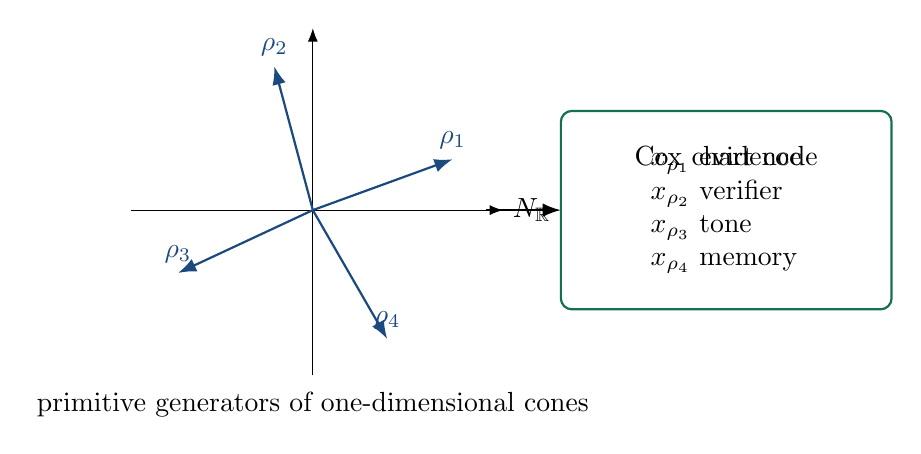
\begin{tikzpicture}[scale=1.05,>=Latex]
\draw[->] (-2.2,0)--(2.3,0) node[right]{$N_\RR$};
\draw[->] (0,-2.0)--(0,2.2);
\foreach \ang/\name in {20/$\rho_1$,105/$\rho_2$,205/$\rho_3$,300/$\rho_4$}{
  \draw[darkblue,thick,->] (0,0)--({1.8*cos(\ang)},{1.8*sin(\ang)}) node[above] {\name};
}
\node[align=center] at (0,-2.35) {primitive generators of one-dimensional cones};
\draw[rounded corners,draw=darkgreen,thick] (3.0,-1.2) rectangle (7.0,1.2);
\node[align=center] at (5,0.65) {Cox chart code};
\node[align=left] at (5,0.0) {$x_{\rho_1}$ evidence\\$x_{\rho_2}$ verifier\\$x_{\rho_3}$ tone\\$x_{\rho_4}$ memory};
\draw[->,thick] (2.1,0)--(3.0,0);
\end{tikzpicture}
\caption{Toric chart code. One-dimensional cones index Cox variables and boundary divisors for evidence, verifier, tone, and memory controls.}
\end{figure}

\section{Training methodology and implementation}
\subsection{Step construction and caching}
A ToricGT II training example contains ordinary input/output bytes plus optional graph, proof, verifier, behavior, and certificate metadata. The step builder performs:
\begin{enumerate}
\item segment a trajectory into standardized steps;
\item pad tokens and embeddings to $(n_\star,d)$;
\item compute GraphCG coordinates $\xi=B^\top H$;
\item build filtered complexes on CPU for selected windows;
\item convert finite grids to sparse boundary matrices and multigraded module summaries;
\item cache exact certificates by hash;
\item stream only compact tensors to the GPU;
\item log bits-per-byte, verifier accuracy, artifact bytes, and exact/surrogate agreement.
\end{enumerate}

\subsection{Composite objective}
The base objective is always the prequential byte loss:
\begin{equation}
\loss_{\bitsperbyte}=-\frac1T\sum_{t=1}^T\log_2 q_\theta(b_t\mid b_{<t}).
\end{equation}
Auxiliary losses are staged:
\begin{equation}
\loss=\loss_{\bitsperbyte}+\lambda_{\rm graph}\loss_{\rm graph}+\sum_j \lambda_j(s)\loss_j,
\end{equation}
where
\begin{equation}
\lambda_j(s)>0\Rightarrow \widehat{\Delta\bitsperbyte}_j> -\delta_{\rm tol},\quad \mathrm{audit}_j=\mathrm{pass},\quad \mathrm{artifact}_j\le \mathrm{budget}.
\end{equation}
A teacher model may optimize structure more aggressively. The deployable student is controlled by a bits-per-byte-transfer controller. Structure earns bytes only if it improves validation log score after quantized export or gives a predeclared reasoning gain without statistically meaningful bits-per-byte regression.

\section{Catalogue overview}
The catalogue has two parts. Part I reselects 20 objectives from the previous toric-objective list and rewrites them for dynamical persistence. Part II adds 20 objectives designed specifically for ToricGT II. Each page states the mathematical object, the loss or metric, why it can improve bits-per-byte, reasoning, and control, and how to integrate it.

\begin{longtable}{p{0.07\textwidth}p{0.42\textwidth}p{0.43\textwidth}}
\toprule
ID & Objective & Primary role in ToricGT II\\
\midrule
\endhead
A1 & Dynamic prequential bits-per-byte lift gate & promotion controller for all structure\\
A2 & Step Certificate Conditional Information & entropy criterion for prefix-visible certificates\\
A3 & Toric Partition Entropy and Fan-Margin Loss & stable active-face dynamics\\
A4 & Multistep Saturated Semigroup MDL & nonnormal dictionary-hole control\\
A5 & Hilbert-Basis Trajectory Code Sparsity & minimal reasoning primitive code\\
A6 & Dynamic Toric-Ideal Binomial Consistency & algebraic equivalence across steps\\
A7 & Cox-Degree Persistence Conservation & multigraded behavior/evidence invariants\\
A8 & Cartier Support-Function Slope Dynamics & reusable piecewise-linear proof slopes\\
A9 & Quantized Moment-Map Ergodic Code & compact active geometry summary\\
A10 & Stanley-Reisner Persistence Nonface Loss & forbidden coactivation suppression\\
A11 & Cech Reasoning-Sheaf Gluing Loss & local-to-global coherence\\
A12 & Vector-Bundle Transition Dynamics & tone/personality chart transport\\
A13 & Klyachko-Style Filtration Bundle Compression & expert subspace compression\\
A14 & Differential-Form Conservative Reasoning Loss & path-independent evidence accumulation\\
A15 & Secondary-Fan Markov-Partition Loss & stable chamber transitions\\
A16 & Gale-Dual Persistence Transfer & dual task sharing\\
A17 & Young-Tableau Schur Code Dynamics & compact representation-composition certificates\\
A18 & Littlewood-Richardson Trajectory Composition & associative proof-plan composition\\
A19 & Derived BGG Chain-Map Lift & homological dynamics\\
A20 & Ergodic bits-per-byte-safe Pareto controller & long-run multi-objective gate\\
\midrule
N1 & Step-Packet Standardization Objective & consistent topology from variable reasoning chunks\\
N2 & Persistence Entropy-Rate Loss & lower irrelevant trajectory entropy\\
N3 & Betti Drift and Lifetime Stability & stable reasoning topology\\
N4 & Derived Mapping-Cone Residual & exact failure measurement for transitions\\
N5 & Invariant Occupation-Measure Matching & behavior distribution control\\
N6 & Ergodic Variance Regularizer & reduce long-run instability\\
N7 & Symbolic Toric Entropy Gate & bound active-cell complexity\\
N8 & Multigraded Hilbert-Series Predictor & anticipate output length and proof burden\\
N9 & Leray Memory Direct-Image Objective & compress retrieved local reasoning\\
N10 & Logarithmic-Form Boundary Residue Loss & controlled behavior near safety/evidence divisors\\
N11 & Connection Holonomy Corridor Loss & coherent tone/personality transport\\
N12 & Crystal-Graph Reasoning Dynamics & root-system step control\\
N13 & Weyl-Chamber Reflection Equivariance & robust symmetric task transfer\\
N14 & Tableau Normal-Form Compression Loss & canonicalize combinatorial reasoning\\
N15 & Toroidal Slepian Concentration Objective & phase-memory bandwidth control\\
N16 & Persistence Lifetime Commitment Gate & answer only when features are stable\\
N17 & Chain-Recurrent Error-Pruning Metric & detect attractors of bad reasoning\\
N18 & Mixing-Time and Regeneration Diagnostic & distinguish robust dynamics from memorization\\
N19 & Spectral-Sequence Collapse Supervision & multiscale sheaf computation control\\
N20 & Minimal-Resolution Complexity Predictor & bits-per-byte-aware homological budget\\
\bottomrule
\end{longtable}
\clearpage
\section{Part I: Twenty reselected ToricGT objectives rewritten for dynamical persistence}
\clearpage
\subsection{A1. Dynamic prequential bits-per-byte lift gate}
\noindent\textbf{Definition and loss.} The original bits-per-byte lift gate becomes a dynamical promotion rule. For an auxiliary family $j$, define a per-step side code $Z^j_t$ extracted from the current standardized packet and its strict prefix. Let $q_{0}$ be the base predictor and $q_j$ the predictor with the auxiliary enabled. The logged lift is
\[
\widehat{\Delta\bitsperbyte}_j=\frac1T\sum_{t=1}^T\log_2\frac{q_j(b_t\mid\mathcal F_t)}{q_0(b_t\mid\mathcal F_t)}.
\]
The objective is not a differentiable loss by itself; it is a controller:
\[
\lambda_j(s+1)=\lambda_j(s)\,\mathbf 1\{\widehat{\Delta\bitsperbyte}_j> -\delta,\;a_j<a_{\max},\;\mathrm{audit}_j=1\}+\eps_j\mathbf 1\{\widehat{\Delta\bitsperbyte}_j>\eta\}.
\]
Here $a_j$ is artifact-byte risk and $\mathrm{audit}_j$ includes exact-small-window agreement.

\noindent\textbf{Why it can improve bits-per-byte, reasoning, and control.} The compression argument is the conditional-information theorem: an auxiliary helps optimal bits-per-byte only through prefix-visible information about the next byte. Dynamical certificates are therefore promoted only after they help the actual emitted sequence, not merely after they look mathematically coherent. This prevents topological or toric plots from steering a compact model away from its score objective.

\noindent\textbf{Training integration and audit.} Integration is straightforward. Every training run logs matched-seed bits-per-byte, quantized-export bits-per-byte, reasoning accuracy, corridor violations, and exact/surrogate agreement. The gate is applied per family: persistence, toric fan, Cech sheaf, tableau, root-system, bundle, ergodic, and derived losses. During teacher training the gate may be loose; during student compression it is strict. A family that improves proof accuracy but harms bits-per-byte can remain in reranking, verifier, or teacher distillation, but not in the serialized bits-per-byte student.

For control, the same gate logs slice scores: formal math, code, natural prose, safety/tone tasks, and long-context retrieval. A loss is unsafe if it improves algebra slices by overfitting style while degrading ordinary prose. The final metric is not aesthetic structure; it is score-valid, export-valid, slice-stable bits-per-byte lift with no unacceptable reasoning regression.

\noindent\textbf{Pragmatic computation.} In a minibatch, materialize only the tensors needed by this objective: the hidden step table $H_t$, a small certificate tensor $C_t$, a transition or transport matrix $F_t$ when the objective is dynamical, and a scalar prefix-visible summary $Z_t$ for the bits-per-byte head. The exact object is built or refreshed on CPU for a sampled subset and cached by a hash of the graph, chart, and threshold grid. The GPU surrogate is intentionally low rank: a few logits, sparse boundary entries, quantized cell ids, or small moment vectors. Every update logs four numbers for this objective: surrogate residual, exact residual, conditional-information lift, and verifier or behavior-corridor delta. If exact and soft residuals decorrelate, the loss is frozen and demoted to audit-only.

\noindent\textbf{Minimal working example.} Use a three-step trajectory with five factors per step: evidence, plan, verifier, memory, and style. Build a two-level filtration with thresholds $\rho_1<\rho_2$, compute $C_1\to C_0$ and optionally $C_2\to C_1$, attach a one-dimensional-cone fan-cell id to each factor, and predict the next byte with and without the certificate summary. The objective is useful only if the certificate improves the log probability of held-out continuations such as equation tokens, citation markers, final-answer phrases, or calibrated caveats. This miniature example is small enough to audit exactly over $\FF_2$ and large enough to detect branch/merge inconsistencies.

\noindent\textbf{Failure modes and ablations.} The common false positive is structural collapse: entropy falls because the model stops exploring, not because it reasons better. A second failure is style leakage: a tone/personality code improves a narrow behavior slice while degrading ordinary prose. A third failure is artifact inflation: the teacher improves but the student loses after quantization or serialization. The required ablation compares base, shuffled-certificate, teacher-certificate, and distilled-student variants under matched seeds. Report global bits-per-byte, slice bits-per-byte, answer accuracy, verifier calibration, corridor violation rate, artifact bytes, and exact audit agreement before promotion.
\vfill
\noindent\emph{Promotion rule.} Keep this objective audit-only until exact small-window checks agree with the differentiable surrogate; enable it in the teacher when verifier or reasoning metrics improve; export it only when quantized bits-per-byte is nondegrading and slice-level behavior remains within the declared corridor.
\clearpage
\subsection{A2. Step Certificate Conditional Information}
\noindent\textbf{Definition and loss.} This objective estimates whether a step-level certificate actually carries predictive information. Let $Z_t$ be a certificate such as a Betti vector, active fan cell, Cox degree, tableau id, or bundle-transition label. Train a lightweight estimator of
\[
I(B_t;Z_t\mid\mathcal F_t)=\Ent(B_t\mid\mathcal F_t)-\Ent(B_t\mid\mathcal F_t,Z_t).
\]
A practical lower-bound proxy is the log-loss gap between a base head and a side-code head:
\[
\loss_{\rm CCI}=-\frac1T\sum_t\log q_Z(b_t\mid h_t,Z_t)+\frac1T\sum_t\log q_0(b_t\mid h_t),
\]
reported in bits. Positive lift means the certificate lowers conditional entropy.

\noindent\textbf{Why it can improve bits-per-byte, reasoning, and control.} The reasoning argument is that structural certificates should canonicalize hidden states. If two proof routes have the same persistence signature and lead to the same answer style, their next-token distributions should be closer. If the certificate is independent of the next byte, it should be suppressed. This turns certificate selection into an information bottleneck rather than a taste judgment.

\noindent\textbf{Training integration and audit.} Training uses three heads: base, certificate-aware, and shuffled-certificate. The shuffled head estimates spurious capacity. A valid certificate must beat both base and shuffled controls. For tone/personality control, $Z_t$ can be a corridor id or residue label; it is useful only if it predicts appropriate surface form and verifier-valid caution without leaking future labels.

The export rule is conservative. If $Z_t$ requires a large module, distill its effect into hidden states or a small codebook. Keep the explicit certificate only when its conditional-information gain remains after quantized round-trip evaluation. This objective is especially useful for deciding whether persistence diagrams, tableaux, or sheaf-gluing indicators should enter a small model.

\noindent\textbf{Pragmatic computation.} In a minibatch, materialize only the tensors needed by this objective: the hidden step table $H_t$, a small certificate tensor $C_t$, a transition or transport matrix $F_t$ when the objective is dynamical, and a scalar prefix-visible summary $Z_t$ for the bits-per-byte head. The exact object is built or refreshed on CPU for a sampled subset and cached by a hash of the graph, chart, and threshold grid. The GPU surrogate is intentionally low rank: a few logits, sparse boundary entries, quantized cell ids, or small moment vectors. Every update logs four numbers for this objective: surrogate residual, exact residual, conditional-information lift, and verifier or behavior-corridor delta. If exact and soft residuals decorrelate, the loss is frozen and demoted to audit-only.

\noindent\textbf{Minimal working example.} Use a three-step trajectory with five factors per step: evidence, plan, verifier, memory, and style. Build a two-level filtration with thresholds $\rho_1<\rho_2$, compute $C_1\to C_0$ and optionally $C_2\to C_1$, attach a one-dimensional-cone fan-cell id to each factor, and predict the next byte with and without the certificate summary. The objective is useful only if the certificate improves the log probability of held-out continuations such as equation tokens, citation markers, final-answer phrases, or calibrated caveats. This miniature example is small enough to audit exactly over $\FF_2$ and large enough to detect branch/merge inconsistencies.

\noindent\textbf{Failure modes and ablations.} The common false positive is structural collapse: entropy falls because the model stops exploring, not because it reasons better. A second failure is style leakage: a tone/personality code improves a narrow behavior slice while degrading ordinary prose. A third failure is artifact inflation: the teacher improves but the student loses after quantization or serialization. The required ablation compares base, shuffled-certificate, teacher-certificate, and distilled-student variants under matched seeds. Report global bits-per-byte, slice bits-per-byte, answer accuracy, verifier calibration, corridor violation rate, artifact bytes, and exact audit agreement before promotion.
\vfill
\noindent\emph{Promotion rule.} Keep this objective audit-only until exact small-window checks agree with the differentiable surrogate; enable it in the teacher when verifier or reasoning metrics improve; export it only when quantized bits-per-byte is nondegrading and slice-level behavior remains within the declared corridor.
\clearpage
\subsection{A3. Toric Partition Entropy and Fan-Margin Loss}
\noindent\textbf{Definition and loss.} A tropical or ReLU subnetwork induces a normal-fan partition of hidden chart space. Let $C_t\in\{1,\ldots,R\}$ be the active cell and let $\Delta_t$ be the top-two margin to the nearest wall. Define
\[
\loss_{\rm fan}=\beta_H H(C_{t+1}\mid C_t,\mathrm{task})+\beta_M\mathbb E\max(0,\gamma-\Delta_t)+\beta_J\|P(C_{t+1}\mid C_t)-\widehat P_{\rm target}\|_F^2.
\]
This is not a universal entropy minimizer. It reduces entropy only within equivalence classes where the verifier says the same reasoning mode should be reused.

\noindent\textbf{Why it can improve bits-per-byte, reasoning, and control.} Compression improves when irrelevant hidden branch choices collapse into stable cell codes. If the same algebraic proof step can be written through many unstable active faces, the next-byte distribution becomes diffuse. A margin-stable fan cell gives the decoder a reusable code for local reasoning mode, expected notation, and tone.

\noindent\textbf{Training integration and audit.} For iterative trajectories, $C_t$ is treated as a symbolic process. The transition entropy rate is logged alongside bits-per-byte. Low fan entropy with low accuracy indicates collapse; high fan entropy with high bits-per-byte indicates unnecessary mode noise. The desired regime is low entropy for routine transformations and controlled entropy for genuine branching.

Implementation uses low-rank probes with rational-quantized slopes. The exact audit recomputes active faces and margins on CPU. The differentiable loss uses softmax temperature and hinge margins. Behavior control is included by refining cells with corridor labels: evidence-scarce cells must prefer cautious tone, while high-verifier cells may allow concise confident exposition.

\noindent\textbf{Pragmatic computation.} In a minibatch, materialize only the tensors needed by this objective: the hidden step table $H_t$, a small certificate tensor $C_t$, a transition or transport matrix $F_t$ when the objective is dynamical, and a scalar prefix-visible summary $Z_t$ for the bits-per-byte head. The exact object is built or refreshed on CPU for a sampled subset and cached by a hash of the graph, chart, and threshold grid. The GPU surrogate is intentionally low rank: a few logits, sparse boundary entries, quantized cell ids, or small moment vectors. Every update logs four numbers for this objective: surrogate residual, exact residual, conditional-information lift, and verifier or behavior-corridor delta. If exact and soft residuals decorrelate, the loss is frozen and demoted to audit-only.

\noindent\textbf{Minimal working example.} Use a three-step trajectory with five factors per step: evidence, plan, verifier, memory, and style. Build a two-level filtration with thresholds $\rho_1<\rho_2$, compute $C_1\to C_0$ and optionally $C_2\to C_1$, attach a one-dimensional-cone fan-cell id to each factor, and predict the next byte with and without the certificate summary. The objective is useful only if the certificate improves the log probability of held-out continuations such as equation tokens, citation markers, final-answer phrases, or calibrated caveats. This miniature example is small enough to audit exactly over $\FF_2$ and large enough to detect branch/merge inconsistencies.

\noindent\textbf{Failure modes and ablations.} The common false positive is structural collapse: entropy falls because the model stops exploring, not because it reasons better. A second failure is style leakage: a tone/personality code improves a narrow behavior slice while degrading ordinary prose. A third failure is artifact inflation: the teacher improves but the student loses after quantization or serialization. The required ablation compares base, shuffled-certificate, teacher-certificate, and distilled-student variants under matched seeds. Report global bits-per-byte, slice bits-per-byte, answer accuracy, verifier calibration, corridor violation rate, artifact bytes, and exact audit agreement before promotion.
\vfill
\noindent\emph{Promotion rule.} Keep this objective audit-only until exact small-window checks agree with the differentiable surrogate; enable it in the teacher when verifier or reasoning metrics improve; export it only when quantized bits-per-byte is nondegrading and slice-level behavior remains within the declared corridor.
\clearpage
\subsection{A4. Multistep Saturated Semigroup MDL}
\noindent\textbf{Definition and loss.} At each step, the model's discrete reasoning primitives generate an affine semigroup $S_t\subset M$. Across a trajectory, valid composition should not create persistent holes: if $k m\in S_t$ for some $k>0$ and $m$ is representable in the ambient lattice, then $m$ should either be available or explicitly marked as disallowed. The loss estimates saturation defects:
\[
\loss_{\rm sat}=\sum_{t}\sum_{m\in\mathcal H_t} w_m\,\mathbf 1\{k_m m\in S_t,\;m\notin S_t\}\,c_m,
\]
where $\mathcal H_t$ is a sampled Hilbert-basis/normalization audit set.

\noindent\textbf{Why it can improve bits-per-byte, reasoning, and control.} The bits-per-byte rationale is minimum description length. Nonnormal hidden dictionaries require exception handling: the model learns many surface forms for missing intermediate concepts. Saturation fills useful intermediate reasoning primitives, reducing irregular conditional distributions. This is particularly relevant for algebraic manipulations, code transformations, and multi-step proof plans.

\noindent\textbf{Training integration and audit.} Dynamically, $S_t$ evolves under $T_\theta$. We penalize holes that persist across many steps more than transient exploratory gaps:
\[
\loss_{\rm dynsat}=\sum_m \mathrm{life}(m)\,\mathrm{hole}(m).
\]
A hole with long lifetime means the model repeatedly needs a concept but refuses to represent it compactly.

Integration uses CPU normalization on small sampled semigroups and a GPU surrogate based on degree-closure prediction. For tone control, behavior primitives such as ``uncertain evidence'', ``safe alternative'', and ``citation required'' are treated as semigroup generators; saturation prevents combinations like high confidence plus low evidence from being represented only through ad hoc exceptions.

\noindent\textbf{Pragmatic computation.} In a minibatch, materialize only the tensors needed by this objective: the hidden step table $H_t$, a small certificate tensor $C_t$, a transition or transport matrix $F_t$ when the objective is dynamical, and a scalar prefix-visible summary $Z_t$ for the bits-per-byte head. The exact object is built or refreshed on CPU for a sampled subset and cached by a hash of the graph, chart, and threshold grid. The GPU surrogate is intentionally low rank: a few logits, sparse boundary entries, quantized cell ids, or small moment vectors. Every update logs four numbers for this objective: surrogate residual, exact residual, conditional-information lift, and verifier or behavior-corridor delta. If exact and soft residuals decorrelate, the loss is frozen and demoted to audit-only.

\noindent\textbf{Minimal working example.} Use a three-step trajectory with five factors per step: evidence, plan, verifier, memory, and style. Build a two-level filtration with thresholds $\rho_1<\rho_2$, compute $C_1\to C_0$ and optionally $C_2\to C_1$, attach a one-dimensional-cone fan-cell id to each factor, and predict the next byte with and without the certificate summary. The objective is useful only if the certificate improves the log probability of held-out continuations such as equation tokens, citation markers, final-answer phrases, or calibrated caveats. This miniature example is small enough to audit exactly over $\FF_2$ and large enough to detect branch/merge inconsistencies.

\noindent\textbf{Failure modes and ablations.} The common false positive is structural collapse: entropy falls because the model stops exploring, not because it reasons better. A second failure is style leakage: a tone/personality code improves a narrow behavior slice while degrading ordinary prose. A third failure is artifact inflation: the teacher improves but the student loses after quantization or serialization. The required ablation compares base, shuffled-certificate, teacher-certificate, and distilled-student variants under matched seeds. Report global bits-per-byte, slice bits-per-byte, answer accuracy, verifier calibration, corridor violation rate, artifact bytes, and exact audit agreement before promotion.
\vfill
\noindent\emph{Promotion rule.} Keep this objective audit-only until exact small-window checks agree with the differentiable surrogate; enable it in the teacher when verifier or reasoning metrics improve; export it only when quantized bits-per-byte is nondegrading and slice-level behavior remains within the declared corridor.
\clearpage
\subsection{A5. Hilbert-Basis Trajectory Code Sparsity}
\noindent\textbf{Definition and loss.} The Hilbert basis of a saturated affine semigroup is the minimal additive dictionary of irreducible lattice elements. ToricGT II uses this as a code for reusable reasoning moves. Let $g_1,\ldots,g_K$ be candidate primitive moves and let $a_{t,k}\ge0$ be soft usage weights with step displacement $\delta_t\approx\sum_k a_{t,k}g_k$. The loss is
\[
\loss_{\rm HB}=\sum_t\|\delta_t-\sum_k a_{t,k}g_k\|^2+\lambda_1\sum_{t,k}|a_{t,k}|+\lambda_{\rm irr}\sum_k \mathrm{reducible}(g_k).
\]

\noindent\textbf{Why it can improve bits-per-byte, reasoning, and control.} The compression mechanism is dictionary sparsity. A proof trajectory represented by many dense latent directions costs more parameters and creates more next-token ambiguity. A Hilbert-basis-like code decomposes it into few canonical moves: introduce lemma, apply relation, verify condition, adjust tone, cite evidence, conclude.

\noindent\textbf{Training integration and audit.} For iterative dynamics, the objective is applied to differences $z_{t+1}-z_t$ in GraphCG/toric coordinates and to changes in persistence-module Betti vectors. If the same displacement recurs, it should reuse the same primitive. This encourages recurrence sharing and improves long-context consistency.

Exact audits compute irreducibility in small lattice cones. Surrogates use nonnegative sparse coding with integer rounding. The codebook may be teacher-only; for deployment, only a tiny quantized move vocabulary is retained if bits-per-byte improves. In behavior control, separate primitive sets are maintained for factual evidence, proof structure, and tone/personality axes, preventing style moves from masquerading as evidence moves.

\noindent\textbf{Pragmatic computation.} In a minibatch, materialize only the tensors needed by this objective: the hidden step table $H_t$, a small certificate tensor $C_t$, a transition or transport matrix $F_t$ when the objective is dynamical, and a scalar prefix-visible summary $Z_t$ for the bits-per-byte head. The exact object is built or refreshed on CPU for a sampled subset and cached by a hash of the graph, chart, and threshold grid. The GPU surrogate is intentionally low rank: a few logits, sparse boundary entries, quantized cell ids, or small moment vectors. Every update logs four numbers for this objective: surrogate residual, exact residual, conditional-information lift, and verifier or behavior-corridor delta. If exact and soft residuals decorrelate, the loss is frozen and demoted to audit-only.

\noindent\textbf{Minimal working example.} Use a three-step trajectory with five factors per step: evidence, plan, verifier, memory, and style. Build a two-level filtration with thresholds $\rho_1<\rho_2$, compute $C_1\to C_0$ and optionally $C_2\to C_1$, attach a one-dimensional-cone fan-cell id to each factor, and predict the next byte with and without the certificate summary. The objective is useful only if the certificate improves the log probability of held-out continuations such as equation tokens, citation markers, final-answer phrases, or calibrated caveats. This miniature example is small enough to audit exactly over $\FF_2$ and large enough to detect branch/merge inconsistencies.

\noindent\textbf{Failure modes and ablations.} The common false positive is structural collapse: entropy falls because the model stops exploring, not because it reasons better. A second failure is style leakage: a tone/personality code improves a narrow behavior slice while degrading ordinary prose. A third failure is artifact inflation: the teacher improves but the student loses after quantization or serialization. The required ablation compares base, shuffled-certificate, teacher-certificate, and distilled-student variants under matched seeds. Report global bits-per-byte, slice bits-per-byte, answer accuracy, verifier calibration, corridor violation rate, artifact bytes, and exact audit agreement before promotion.
\vfill
\noindent\emph{Promotion rule.} Keep this objective audit-only until exact small-window checks agree with the differentiable surrogate; enable it in the teacher when verifier or reasoning metrics improve; export it only when quantized bits-per-byte is nondegrading and slice-level behavior remains within the declared corridor.
\clearpage
\subsection{A6. Dynamic Toric-Ideal Binomial Consistency}
\noindent\textbf{Definition and loss.} A toric ideal records equal monomial parameterizations. If $A=\{a_i\}\subset M$ and $\sum_i u_i a_i=\sum_i v_i a_i$, then $x^u-x^v$ should vanish. For hidden nonnegative chart variables $x_i(t)$, define
\[
\loss_{\rm bin}(t)=\sum_{(u,v)\in\mathcal R}\left(\sum_i u_i\log(x_i(t)+\eps)-\sum_i v_i\log(x_i(t)+\eps)\right)^2.
\]
The dynamic version adds transition consistency:
\[
\loss_{\rm dynbin}=\sum_t\|B(x_{t+1})-\Phi_B(B(x_t))\|^2,
\]
where $B$ is the vector of binomial residuals.

\noindent\textbf{Why it can improve bits-per-byte, reasoning, and control.} bits-per-byte improves when algebraically equivalent continuations receive similar probabilities. Without binomial consistency, the model may waste capacity memorizing different strings for equivalent transformations. With consistency, it can share logits across equivalent proof paths and code paths.

\noindent\textbf{Training integration and audit.} This objective is useful for reasoning accuracy because binomial relations detect invalid symbolic shortcuts. If a hidden state claims two algebraic routes are equivalent, the residual must be small; if it crosses a wall where equivalence no longer holds, the transition is explicit.

Implementation uses a small relation basis from CPU algebra packages or synthetic toric tasks. The GPU sees a short list of integer exponent pairs. For tone control, binomial relations can also tie behavior coordinates: for example, ``safe refusal plus safe alternative'' should match a product of caution and helpfulness variables, while high-confidence/no-evidence is excluded by a separate Stanley-Reisner nonface loss.

\noindent\textbf{Pragmatic computation.} In a minibatch, materialize only the tensors needed by this objective: the hidden step table $H_t$, a small certificate tensor $C_t$, a transition or transport matrix $F_t$ when the objective is dynamical, and a scalar prefix-visible summary $Z_t$ for the bits-per-byte head. The exact object is built or refreshed on CPU for a sampled subset and cached by a hash of the graph, chart, and threshold grid. The GPU surrogate is intentionally low rank: a few logits, sparse boundary entries, quantized cell ids, or small moment vectors. Every update logs four numbers for this objective: surrogate residual, exact residual, conditional-information lift, and verifier or behavior-corridor delta. If exact and soft residuals decorrelate, the loss is frozen and demoted to audit-only.

\noindent\textbf{Minimal working example.} Use a three-step trajectory with five factors per step: evidence, plan, verifier, memory, and style. Build a two-level filtration with thresholds $\rho_1<\rho_2$, compute $C_1\to C_0$ and optionally $C_2\to C_1$, attach a one-dimensional-cone fan-cell id to each factor, and predict the next byte with and without the certificate summary. The objective is useful only if the certificate improves the log probability of held-out continuations such as equation tokens, citation markers, final-answer phrases, or calibrated caveats. This miniature example is small enough to audit exactly over $\FF_2$ and large enough to detect branch/merge inconsistencies.

\noindent\textbf{Failure modes and ablations.} The common false positive is structural collapse: entropy falls because the model stops exploring, not because it reasons better. A second failure is style leakage: a tone/personality code improves a narrow behavior slice while degrading ordinary prose. A third failure is artifact inflation: the teacher improves but the student loses after quantization or serialization. The required ablation compares base, shuffled-certificate, teacher-certificate, and distilled-student variants under matched seeds. Report global bits-per-byte, slice bits-per-byte, answer accuracy, verifier calibration, corridor violation rate, artifact bytes, and exact audit agreement before promotion.
\vfill
\noindent\emph{Promotion rule.} Keep this objective audit-only until exact small-window checks agree with the differentiable surrogate; enable it in the teacher when verifier or reasoning metrics improve; export it only when quantized bits-per-byte is nondegrading and slice-level behavior remains within the declared corridor.
\clearpage
\subsection{A7. Cox-Degree Persistence Conservation}
\noindent\textbf{Definition and loss.} Cox coordinates carry a class-group grading. ToricGT II treats evidence type, proof obligation, verifier state, tone, and safety mode as multigraded charges. Let $d_t\in G$ be the predicted degree of a reasoning step and $\Delta_t$ the transition degree. Conservation is
\[
\loss_{\rm Cox}=\sum_t\|d_{t+1}-d_t-\Delta_t\|_G^2+\lambda_{\rm invalid}\,\mathbf 1\{x_t\in V(B(\Sigma))\},
\]
where $B(\Sigma)$ is the irrelevant ideal defining invalid Cox-coordinate regions.

\noindent\textbf{Why it can improve bits-per-byte, reasoning, and control.} Compression improves because degree conservation reduces mode ambiguity. The decoder can condition on a compact multidegree rather than on a large hidden cloud. A proof step with degree ``lemma/evidence/high-rigor/neutral-tone'' should have a predictable family of next tokens.

\noindent\textbf{Training integration and audit.} In persistence modules, Cox degrees decorate generators. A morphism that changes homological degree but not the appropriate Cox charge is suspicious. The loss therefore couples to Betti tables:
\[
\loss_{\rm BettiCox}=\sum_{i,\alpha,g}|\widehat\beta_{i,\alpha,g}-\beta_{i,\alpha,g}^\star|.
\]

Training integration is cheap: degree labels are small integer vectors. Exact audits check degree addition and invalid chart occupancy. For tone/personality control, degrees separate stylistic shifts from factual shifts. A model may become warmer without changing evidence degree; it may become more cautious when evidence degree is low; it should not increase factual-confidence degree solely through style.

\noindent\textbf{Pragmatic computation.} In a minibatch, materialize only the tensors needed by this objective: the hidden step table $H_t$, a small certificate tensor $C_t$, a transition or transport matrix $F_t$ when the objective is dynamical, and a scalar prefix-visible summary $Z_t$ for the bits-per-byte head. The exact object is built or refreshed on CPU for a sampled subset and cached by a hash of the graph, chart, and threshold grid. The GPU surrogate is intentionally low rank: a few logits, sparse boundary entries, quantized cell ids, or small moment vectors. Every update logs four numbers for this objective: surrogate residual, exact residual, conditional-information lift, and verifier or behavior-corridor delta. If exact and soft residuals decorrelate, the loss is frozen and demoted to audit-only.

\noindent\textbf{Minimal working example.} Use a three-step trajectory with five factors per step: evidence, plan, verifier, memory, and style. Build a two-level filtration with thresholds $\rho_1<\rho_2$, compute $C_1\to C_0$ and optionally $C_2\to C_1$, attach a one-dimensional-cone fan-cell id to each factor, and predict the next byte with and without the certificate summary. The objective is useful only if the certificate improves the log probability of held-out continuations such as equation tokens, citation markers, final-answer phrases, or calibrated caveats. This miniature example is small enough to audit exactly over $\FF_2$ and large enough to detect branch/merge inconsistencies.

\noindent\textbf{Failure modes and ablations.} The common false positive is structural collapse: entropy falls because the model stops exploring, not because it reasons better. A second failure is style leakage: a tone/personality code improves a narrow behavior slice while degrading ordinary prose. A third failure is artifact inflation: the teacher improves but the student loses after quantization or serialization. The required ablation compares base, shuffled-certificate, teacher-certificate, and distilled-student variants under matched seeds. Report global bits-per-byte, slice bits-per-byte, answer accuracy, verifier calibration, corridor violation rate, artifact bytes, and exact audit agreement before promotion.
\vfill
\noindent\emph{Promotion rule.} Keep this objective audit-only until exact small-window checks agree with the differentiable surrogate; enable it in the teacher when verifier or reasoning metrics improve; export it only when quantized bits-per-byte is nondegrading and slice-level behavior remains within the declared corridor.
\clearpage
\subsection{A8. Cartier Support-Function Slope Dynamics}
\noindent\textbf{Definition and loss.} A torus-invariant Cartier divisor has a piecewise-linear support function with slope data on cones. A reasoning trajectory has analogous local slopes: within a toric cell $\sigma$, a probe output is $\psi_t(h)=\langle m_{\sigma,t},h\rangle+c_{\sigma,t}$. Penalize uncontrolled slope drift:
\[
\loss_{\rm Cart}=\sum_t\|m_{\sigma_{t+1},t+1}-\mathcal T_{\sigma_t\to\sigma_{t+1}}m_{\sigma_t,t}\|^2+\lambda_{\rm bend}\sum_{\tau}\|\mathrm{bend}_\tau-\mathrm{bend}_\tau^\star\|^2.
\]

\noindent\textbf{Why it can improve bits-per-byte, reasoning, and control.} The bits-per-byte mechanism is slope sharing. If local reasoning in equivalent cells uses the same support-function slope, the model reuses a small linear rule rather than relearning dense transformations. This helps proofs and code where local cases differ only by chart.

\noindent\textbf{Training integration and audit.} The reasoning benefit is controlled wall crossing. A bend across a wall should correspond to a meaningful decision: switch active lemma, enter refusal mode, require citation, or select a different tableau channel. Random slope drift is a hallucination risk.

Implementation fits slopes from hidden/input-output pairs or reads them from low-rank probes. Exact audits recompute rationalized slope differences. In behavior control, support functions define corridors whose convexity prevents abrupt personality changes. A warm explanatory mode and a terse theorem-proof mode may live in adjacent cells; the bend should be calibrated, not arbitrary.

\noindent\textbf{Pragmatic computation.} In a minibatch, materialize only the tensors needed by this objective: the hidden step table $H_t$, a small certificate tensor $C_t$, a transition or transport matrix $F_t$ when the objective is dynamical, and a scalar prefix-visible summary $Z_t$ for the bits-per-byte head. The exact object is built or refreshed on CPU for a sampled subset and cached by a hash of the graph, chart, and threshold grid. The GPU surrogate is intentionally low rank: a few logits, sparse boundary entries, quantized cell ids, or small moment vectors. Every update logs four numbers for this objective: surrogate residual, exact residual, conditional-information lift, and verifier or behavior-corridor delta. If exact and soft residuals decorrelate, the loss is frozen and demoted to audit-only.

\noindent\textbf{Minimal working example.} Use a three-step trajectory with five factors per step: evidence, plan, verifier, memory, and style. Build a two-level filtration with thresholds $\rho_1<\rho_2$, compute $C_1\to C_0$ and optionally $C_2\to C_1$, attach a one-dimensional-cone fan-cell id to each factor, and predict the next byte with and without the certificate summary. The objective is useful only if the certificate improves the log probability of held-out continuations such as equation tokens, citation markers, final-answer phrases, or calibrated caveats. This miniature example is small enough to audit exactly over $\FF_2$ and large enough to detect branch/merge inconsistencies.

\noindent\textbf{Failure modes and ablations.} The common false positive is structural collapse: entropy falls because the model stops exploring, not because it reasons better. A second failure is style leakage: a tone/personality code improves a narrow behavior slice while degrading ordinary prose. A third failure is artifact inflation: the teacher improves but the student loses after quantization or serialization. The required ablation compares base, shuffled-certificate, teacher-certificate, and distilled-student variants under matched seeds. Report global bits-per-byte, slice bits-per-byte, answer accuracy, verifier calibration, corridor violation rate, artifact bytes, and exact audit agreement before promotion.
\vfill
\noindent\emph{Promotion rule.} Keep this objective audit-only until exact small-window checks agree with the differentiable surrogate; enable it in the teacher when verifier or reasoning metrics improve; export it only when quantized bits-per-byte is nondegrading and slice-level behavior remains within the declared corridor.
\clearpage
\subsection{A9. Quantized Moment-Map Ergodic Code}
\noindent\textbf{Definition and loss.} Given affine candidates $\ell_r(h)$ with exponent vectors $a_r$, define the soft active moment
\[
\mu_\beta(h)=\frac{\sum_r e^{\beta\ell_r(h)}a_r}{\sum_r e^{\beta\ell_r(h)}}\in\mathrm{Conv}(a_1,\ldots,a_R).
\]
ToricGT II quantizes $\mu_\beta(h_t)$ into a small code $q_t$ and regularizes long-run occupation:
\[
\loss_{\rm mom}=\sum_t\|\mu_\beta(h_t)-\mathrm{code}(q_t)\|^2+\lambda_{\rm occ}\KL(\widehat\pi_q\|\pi_q^\star).
\]

\noindent\textbf{Why it can improve bits-per-byte, reasoning, and control.} This code compresses active geometry. Instead of exporting a large explanation trace, the model can store a few moment ids representing proof mode, evidence status, and tone corridor. The ergodic occupation term prevents the codebook from collapsing to one state or diffusing across too many states.

\noindent\textbf{Training integration and audit.} For reasoning, moment trajectories reveal whether the model moves through expected phases: parse, plan, retrieve, verify, explain. For tone control, moments can track warmth/rigor/caution tradeoffs without exposing private chain text.

Integration uses fake quantization during training and exact integer codebooks at export. A code enters the student only if it improves bits-per-byte or verifier-guided generation. The audit reports moment reconstruction error, transition entropy, slice-specific bits-per-byte lift, and mismatch between teacher and student occupation measures.

\noindent\textbf{Pragmatic computation.} In a minibatch, materialize only the tensors needed by this objective: the hidden step table $H_t$, a small certificate tensor $C_t$, a transition or transport matrix $F_t$ when the objective is dynamical, and a scalar prefix-visible summary $Z_t$ for the bits-per-byte head. The exact object is built or refreshed on CPU for a sampled subset and cached by a hash of the graph, chart, and threshold grid. The GPU surrogate is intentionally low rank: a few logits, sparse boundary entries, quantized cell ids, or small moment vectors. Every update logs four numbers for this objective: surrogate residual, exact residual, conditional-information lift, and verifier or behavior-corridor delta. If exact and soft residuals decorrelate, the loss is frozen and demoted to audit-only.

\noindent\textbf{Minimal working example.} Use a three-step trajectory with five factors per step: evidence, plan, verifier, memory, and style. Build a two-level filtration with thresholds $\rho_1<\rho_2$, compute $C_1\to C_0$ and optionally $C_2\to C_1$, attach a one-dimensional-cone fan-cell id to each factor, and predict the next byte with and without the certificate summary. The objective is useful only if the certificate improves the log probability of held-out continuations such as equation tokens, citation markers, final-answer phrases, or calibrated caveats. This miniature example is small enough to audit exactly over $\FF_2$ and large enough to detect branch/merge inconsistencies.

\noindent\textbf{Failure modes and ablations.} The common false positive is structural collapse: entropy falls because the model stops exploring, not because it reasons better. A second failure is style leakage: a tone/personality code improves a narrow behavior slice while degrading ordinary prose. A third failure is artifact inflation: the teacher improves but the student loses after quantization or serialization. The required ablation compares base, shuffled-certificate, teacher-certificate, and distilled-student variants under matched seeds. Report global bits-per-byte, slice bits-per-byte, answer accuracy, verifier calibration, corridor violation rate, artifact bytes, and exact audit agreement before promotion.
\vfill
\noindent\emph{Promotion rule.} Keep this objective audit-only until exact small-window checks agree with the differentiable surrogate; enable it in the teacher when verifier or reasoning metrics improve; export it only when quantized bits-per-byte is nondegrading and slice-level behavior remains within the declared corridor.
\clearpage
\subsection{A10. Stanley-Reisner Persistence Nonface Loss}
\noindent\textbf{Definition and loss.} A simplicial complex $\Delta$ has a Stanley-Reisner ideal generated by monomials corresponding to nonfaces. In a reasoning step, nonfaces represent incompatible coactivations: high confidence with no evidence, unsafe instruction with warm compliance, proof conclusion without verifier support, or verbose detail under low certainty. Let $x_i(t)\in[0,1]$ be soft activations. The dynamic nonface loss is
\[
\loss_{\rm SR}=\sum_t\sum_{F\notin\Delta_t} w_F\prod_{i\in F}x_i(t)+\lambda_{\rm pers}\sum_{F}\mathrm{life}(F)\prod_{i\in F}x_i(t).
\]

\noindent\textbf{Why it can improve bits-per-byte, reasoning, and control.} The bits-per-byte benefit comes from suppressing contradictory hidden states. Contradictory states lead to high-entropy surface continuations: the model hedges, over-explains, or changes tone mid-answer. Removing invalid coactivations sharpens the next-byte distribution.

\noindent\textbf{Training integration and audit.} The persistence term matters because a transient exploratory conflict may be acceptable, but a long-lived conflict is a bad attractor. A high-confidence/no-evidence nonface with long lifetime should be heavily penalized before decoding.

Implementation maintains a library of nonfaces by domain and behavior policy. Exact audits hard-threshold activations and recompute complex validity. The deployable model may retain only the learned corridor projection, not the full nonface library. This objective is one of the most pragmatic algebraic controls because it translates behavioral policy into monomial constraints.

\noindent\textbf{Pragmatic computation.} In a minibatch, materialize only the tensors needed by this objective: the hidden step table $H_t$, a small certificate tensor $C_t$, a transition or transport matrix $F_t$ when the objective is dynamical, and a scalar prefix-visible summary $Z_t$ for the bits-per-byte head. The exact object is built or refreshed on CPU for a sampled subset and cached by a hash of the graph, chart, and threshold grid. The GPU surrogate is intentionally low rank: a few logits, sparse boundary entries, quantized cell ids, or small moment vectors. Every update logs four numbers for this objective: surrogate residual, exact residual, conditional-information lift, and verifier or behavior-corridor delta. If exact and soft residuals decorrelate, the loss is frozen and demoted to audit-only.

\noindent\textbf{Minimal working example.} Use a three-step trajectory with five factors per step: evidence, plan, verifier, memory, and style. Build a two-level filtration with thresholds $\rho_1<\rho_2$, compute $C_1\to C_0$ and optionally $C_2\to C_1$, attach a one-dimensional-cone fan-cell id to each factor, and predict the next byte with and without the certificate summary. The objective is useful only if the certificate improves the log probability of held-out continuations such as equation tokens, citation markers, final-answer phrases, or calibrated caveats. This miniature example is small enough to audit exactly over $\FF_2$ and large enough to detect branch/merge inconsistencies.

\noindent\textbf{Failure modes and ablations.} The common false positive is structural collapse: entropy falls because the model stops exploring, not because it reasons better. A second failure is style leakage: a tone/personality code improves a narrow behavior slice while degrading ordinary prose. A third failure is artifact inflation: the teacher improves but the student loses after quantization or serialization. The required ablation compares base, shuffled-certificate, teacher-certificate, and distilled-student variants under matched seeds. Report global bits-per-byte, slice bits-per-byte, answer accuracy, verifier calibration, corridor violation rate, artifact bytes, and exact audit agreement before promotion.
\vfill
\noindent\emph{Promotion rule.} Keep this objective audit-only until exact small-window checks agree with the differentiable surrogate; enable it in the teacher when verifier or reasoning metrics improve; export it only when quantized bits-per-byte is nondegrading and slice-level behavior remains within the declared corridor.
\clearpage
\subsection{A11. Cech Reasoning-Sheaf Gluing Loss}
\noindent\textbf{Definition and loss.} Local reasoning windows often live on different toric charts. Let $s_{i,t}\in\Gamma(U_i,\calF)$ be local sections representing evidence, proof fragment, style plan, or memory retrieval on chart $U_i$. The Cech gluing residual is
\[
\loss_{\check C}=\sum_t\sum_{i<j}\|s_{i,t}|_{U_i\cap U_j}-s_{j,t}|_{U_i\cap U_j}\|^2+\\lambda_1\|d^1 d^0 s_t\|^2.
\]
The second term checks the complex identity for the learned overlap maps.

\noindent\textbf{Why it can improve bits-per-byte, reasoning, and control.} Compression improves when local explanations agree on overlaps. Without gluing, the decoder must resolve contradictions at generation time, increasing entropy and hallucination risk. With gluing, the answer can be generated from a global section-like state.

\noindent\textbf{Training integration and audit.} Reasoning quality improves because local correctness is not enough. A proof branch, retrieved citation, and final conclusion may each be plausible but inconsistent. Cech residuals directly measure this local-to-global failure. For tone/personality, each chart may represent behavior axes differently; gluing ensures the same global persona corridor is maintained.

Implementation uses affine chart covers selected by active fan cells. Local sections are low-rank projections, not full text. Exact small audits threshold chart occupancy and compute Cech cochains. The objective is late-stage and teacher-friendly; in a student it is distilled into reduced contradiction rate and lower bits-per-byte on multi-hop explanations.

\noindent\textbf{Pragmatic computation.} In a minibatch, materialize only the tensors needed by this objective: the hidden step table $H_t$, a small certificate tensor $C_t$, a transition or transport matrix $F_t$ when the objective is dynamical, and a scalar prefix-visible summary $Z_t$ for the bits-per-byte head. The exact object is built or refreshed on CPU for a sampled subset and cached by a hash of the graph, chart, and threshold grid. The GPU surrogate is intentionally low rank: a few logits, sparse boundary entries, quantized cell ids, or small moment vectors. Every update logs four numbers for this objective: surrogate residual, exact residual, conditional-information lift, and verifier or behavior-corridor delta. If exact and soft residuals decorrelate, the loss is frozen and demoted to audit-only.

\noindent\textbf{Minimal working example.} Use a three-step trajectory with five factors per step: evidence, plan, verifier, memory, and style. Build a two-level filtration with thresholds $\rho_1<\rho_2$, compute $C_1\to C_0$ and optionally $C_2\to C_1$, attach a one-dimensional-cone fan-cell id to each factor, and predict the next byte with and without the certificate summary. The objective is useful only if the certificate improves the log probability of held-out continuations such as equation tokens, citation markers, final-answer phrases, or calibrated caveats. This miniature example is small enough to audit exactly over $\FF_2$ and large enough to detect branch/merge inconsistencies.

\noindent\textbf{Failure modes and ablations.} The common false positive is structural collapse: entropy falls because the model stops exploring, not because it reasons better. A second failure is style leakage: a tone/personality code improves a narrow behavior slice while degrading ordinary prose. A third failure is artifact inflation: the teacher improves but the student loses after quantization or serialization. The required ablation compares base, shuffled-certificate, teacher-certificate, and distilled-student variants under matched seeds. Report global bits-per-byte, slice bits-per-byte, answer accuracy, verifier calibration, corridor violation rate, artifact bytes, and exact audit agreement before promotion.
\vfill
\noindent\emph{Promotion rule.} Keep this objective audit-only until exact small-window checks agree with the differentiable surrogate; enable it in the teacher when verifier or reasoning metrics improve; export it only when quantized bits-per-byte is nondegrading and slice-level behavior remains within the declared corridor.
\clearpage
\subsection{A12. Vector-Bundle Transition Dynamics}
\noindent\textbf{Definition and loss.} Let $E\to X_\Sigma$ be a rank-$r$ behavior/concept bundle with transition functions $g_{ij}$. Hidden chart coordinates $y_i(t)$ and $y_j(t)$ should satisfy $y_i=g_{ij}y_j$ on overlaps. The loss is
\[
\loss_{\rm vb}=\sum_t\sum_{i<j}\|y_i(t)-g_{ij}(t)y_j(t)\|^2+\lambda_{\rm coc}\sum_{i,j,k}\|g_{ij}g_{jk}g_{ki}-I\|_F^2.
\]

\noindent\textbf{Why it can improve bits-per-byte, reasoning, and control.} This improves bits-per-byte by making concept axes portable. If the model's ``rigor'', ``caution'', ``warmth'', or ``citation demand'' axis changes unpredictably across charts, the decoder sees inconsistent state and spreads probability mass. Bundle transitions make the same behavior vector comparable everywhere.

\noindent\textbf{Training integration and audit.} The reasoning benefit is controlled tonality and personality. Different domains require different local charts: theorem proof, code review, biomedical caution, safety refusal, or tutorial explanation. A vector bundle allows chart-dependent coordinates while enforcing cocycle coherence.

Training uses small matrices, often diagonal-plus-low-rank. Exact audits check cocycles on occupied triple overlaps. A hard gate prevents bundle losses from overriding factual accuracy: if verifier confidence decreases, tone may become cautious, but bundle transport cannot create factual support. Export keeps only low-rank adapters if they improve bits-per-byte or behavior metrics.

\noindent\textbf{Pragmatic computation.} In a minibatch, materialize only the tensors needed by this objective: the hidden step table $H_t$, a small certificate tensor $C_t$, a transition or transport matrix $F_t$ when the objective is dynamical, and a scalar prefix-visible summary $Z_t$ for the bits-per-byte head. The exact object is built or refreshed on CPU for a sampled subset and cached by a hash of the graph, chart, and threshold grid. The GPU surrogate is intentionally low rank: a few logits, sparse boundary entries, quantized cell ids, or small moment vectors. Every update logs four numbers for this objective: surrogate residual, exact residual, conditional-information lift, and verifier or behavior-corridor delta. If exact and soft residuals decorrelate, the loss is frozen and demoted to audit-only.

\noindent\textbf{Minimal working example.} Use a three-step trajectory with five factors per step: evidence, plan, verifier, memory, and style. Build a two-level filtration with thresholds $\rho_1<\rho_2$, compute $C_1\to C_0$ and optionally $C_2\to C_1$, attach a one-dimensional-cone fan-cell id to each factor, and predict the next byte with and without the certificate summary. The objective is useful only if the certificate improves the log probability of held-out continuations such as equation tokens, citation markers, final-answer phrases, or calibrated caveats. This miniature example is small enough to audit exactly over $\FF_2$ and large enough to detect branch/merge inconsistencies.

\noindent\textbf{Failure modes and ablations.} The common false positive is structural collapse: entropy falls because the model stops exploring, not because it reasons better. A second failure is style leakage: a tone/personality code improves a narrow behavior slice while degrading ordinary prose. A third failure is artifact inflation: the teacher improves but the student loses after quantization or serialization. The required ablation compares base, shuffled-certificate, teacher-certificate, and distilled-student variants under matched seeds. Report global bits-per-byte, slice bits-per-byte, answer accuracy, verifier calibration, corridor violation rate, artifact bytes, and exact audit agreement before promotion.
\vfill
\noindent\emph{Promotion rule.} Keep this objective audit-only until exact small-window checks agree with the differentiable surrogate; enable it in the teacher when verifier or reasoning metrics improve; export it only when quantized bits-per-byte is nondegrading and slice-level behavior remains within the declared corridor.
\clearpage
\subsection{A13. Klyachko-Style Filtration Bundle Compression}
\noindent\textbf{Definition and loss.} Toric vector bundles can be described by filtrations indexed by one-dimensional cones. ToricGT II uses an analogous description for expert subspaces. For each one-dimensional cone $\rho$ and integer level $a$, let $E^\rho(a)$ be a nested subspace of a shared expert space $E$. Penalize violations:
\[
\loss_{\rm filt}=\sum_{\rho,a}\max(0,\|\Pi_{E^\rho(a+1)}-\Pi_{E^\rho(a)}\|_{\rm order})+\lambda\sum_t\dist(e_t,E^{\rho_t}(a_t))^2.
\]

\noindent\textbf{Why it can improve bits-per-byte, reasoning, and control.} The compression mechanism is subspace sharing. Instead of storing many experts, the model stores a common space plus cone-indexed filtrations. Routing becomes a small combinatorial code. This is ideal for bits-per-byte-limited students where full Soft-MoE is too expensive.

\noindent\textbf{Training integration and audit.} For reasoning, filtrations encode increasing evidence strength, proof depth, safety strictness, or tone specificity. A step with low evidence lies in a restrictive subspace; a verified proof may access a larger explanatory subspace. The nesting prevents abrupt uncontrolled jumps.

Implementation uses low-rank projection matrices and monotonicity penalties. Exact audits inspect small subspace dimensions and cone labels. The deployable version can be a shared MLP plus tiny filtration gates. This objective is a direct bridge from toric vector-bundle theory to practical parameter sharing.

\noindent\textbf{Pragmatic computation.} In a minibatch, materialize only the tensors needed by this objective: the hidden step table $H_t$, a small certificate tensor $C_t$, a transition or transport matrix $F_t$ when the objective is dynamical, and a scalar prefix-visible summary $Z_t$ for the bits-per-byte head. The exact object is built or refreshed on CPU for a sampled subset and cached by a hash of the graph, chart, and threshold grid. The GPU surrogate is intentionally low rank: a few logits, sparse boundary entries, quantized cell ids, or small moment vectors. Every update logs four numbers for this objective: surrogate residual, exact residual, conditional-information lift, and verifier or behavior-corridor delta. If exact and soft residuals decorrelate, the loss is frozen and demoted to audit-only.

\noindent\textbf{Minimal working example.} Use a three-step trajectory with five factors per step: evidence, plan, verifier, memory, and style. Build a two-level filtration with thresholds $\rho_1<\rho_2$, compute $C_1\to C_0$ and optionally $C_2\to C_1$, attach a one-dimensional-cone fan-cell id to each factor, and predict the next byte with and without the certificate summary. The objective is useful only if the certificate improves the log probability of held-out continuations such as equation tokens, citation markers, final-answer phrases, or calibrated caveats. This miniature example is small enough to audit exactly over $\FF_2$ and large enough to detect branch/merge inconsistencies.

\noindent\textbf{Failure modes and ablations.} The common false positive is structural collapse: entropy falls because the model stops exploring, not because it reasons better. A second failure is style leakage: a tone/personality code improves a narrow behavior slice while degrading ordinary prose. A third failure is artifact inflation: the teacher improves but the student loses after quantization or serialization. The required ablation compares base, shuffled-certificate, teacher-certificate, and distilled-student variants under matched seeds. Report global bits-per-byte, slice bits-per-byte, answer accuracy, verifier calibration, corridor violation rate, artifact bytes, and exact audit agreement before promotion.
\vfill
\noindent\emph{Promotion rule.} Keep this objective audit-only until exact small-window checks agree with the differentiable surrogate; enable it in the teacher when verifier or reasoning metrics improve; export it only when quantized bits-per-byte is nondegrading and slice-level behavior remains within the declared corridor.
\clearpage
\subsection{A14. Differential-Form Conservative Reasoning Loss}
\noindent\textbf{Definition and loss.} Let $\omega=\sum_i f_i(z)dz_i$ be a learned 1-form on GraphCG/toric chart coordinates. It measures infinitesimal evidence or confidence change. Penalize nonconservative accumulation:
\[
\loss_{d\omega}=\mathbb E\|d\omega(z_t)\|_F^2+\lambda_{\rm loop}\sum_{\ell\in\mathcal L}\left|\oint_\ell \omega\right|^2.
\]
For boundary behavior, use logarithmic forms $\omega+\sum_j r_j d\log x_j$ and penalize invalid residues $r_j$ along evidence, refusal, or safety divisors.

\noindent\textbf{Why it can improve bits-per-byte, reasoning, and control.} bits-per-byte improves when confidence and tone are path-independent where the task semantics are path-independent. If two valid proof routes reach the same conclusion but induce different confidence or style, generation becomes unstable. A closed-form penalty makes the endpoint state more canonical.

\noindent\textbf{Training integration and audit.} Reasoning accuracy improves because nonzero loop integral detects circular justification: a trajectory returns to the same evidence state with higher confidence. Logarithmic residues handle boundaries: near low evidence, high-stakes, or unsafe-request divisors, tone should change predictably.

Implementation estimates exterior derivatives by Jacobian-vector products on low-rank chart coordinates. Loop losses use sampled cycles in graph-of-thought DAGs. Exact audits compare route pairs with identical verifier state. The student may retain only the resulting calibrated confidence head.

\noindent\textbf{Pragmatic computation.} In a minibatch, materialize only the tensors needed by this objective: the hidden step table $H_t$, a small certificate tensor $C_t$, a transition or transport matrix $F_t$ when the objective is dynamical, and a scalar prefix-visible summary $Z_t$ for the bits-per-byte head. The exact object is built or refreshed on CPU for a sampled subset and cached by a hash of the graph, chart, and threshold grid. The GPU surrogate is intentionally low rank: a few logits, sparse boundary entries, quantized cell ids, or small moment vectors. Every update logs four numbers for this objective: surrogate residual, exact residual, conditional-information lift, and verifier or behavior-corridor delta. If exact and soft residuals decorrelate, the loss is frozen and demoted to audit-only.

\noindent\textbf{Minimal working example.} Use a three-step trajectory with five factors per step: evidence, plan, verifier, memory, and style. Build a two-level filtration with thresholds $\rho_1<\rho_2$, compute $C_1\to C_0$ and optionally $C_2\to C_1$, attach a one-dimensional-cone fan-cell id to each factor, and predict the next byte with and without the certificate summary. The objective is useful only if the certificate improves the log probability of held-out continuations such as equation tokens, citation markers, final-answer phrases, or calibrated caveats. This miniature example is small enough to audit exactly over $\FF_2$ and large enough to detect branch/merge inconsistencies.

\noindent\textbf{Failure modes and ablations.} The common false positive is structural collapse: entropy falls because the model stops exploring, not because it reasons better. A second failure is style leakage: a tone/personality code improves a narrow behavior slice while degrading ordinary prose. A third failure is artifact inflation: the teacher improves but the student loses after quantization or serialization. The required ablation compares base, shuffled-certificate, teacher-certificate, and distilled-student variants under matched seeds. Report global bits-per-byte, slice bits-per-byte, answer accuracy, verifier calibration, corridor violation rate, artifact bytes, and exact audit agreement before promotion.
\vfill
\noindent\emph{Promotion rule.} Keep this objective audit-only until exact small-window checks agree with the differentiable surrogate; enable it in the teacher when verifier or reasoning metrics improve; export it only when quantized bits-per-byte is nondegrading and slice-level behavior remains within the declared corridor.
\clearpage
\subsection{A15. Secondary-Fan Markov-Partition Loss}
\noindent\textbf{Definition and loss.} Secondary fans organize triangulations, GIT chambers, and wall crossings. In ToricGT II they organize alternative reasoning decompositions. Let $C_t$ be a secondary-fan chamber for the current decomposition and $P_{ij}$ the empirical transition matrix. The loss is
\[
\loss_{\rm sec}=\sum_t \mathrm{wallcost}(C_t,C_{t+1})+\lambda_H H(C_{t+1}\mid C_t,\mathrm{verifier})+\lambda_{\rm flip}\,\mathrm{badflip}_t.
\]

\noindent\textbf{Why it can improve bits-per-byte, reasoning, and control.} Compression improves when equivalent decompositions share a chamber code. The decoder should not need separate parameters for every triangulation-like proof split. Wall crossings are allowed when they correspond to useful flips; random chamber jitter wastes entropy.

\noindent\textbf{Training integration and audit.} Reasoning quality improves because some tasks genuinely require changing decomposition: regrouping terms, changing induction order, or switching graph traversal. The secondary-fan code distinguishes controlled flips from instability.

Implementation obtains chambers from small combinatorial certificates: triangulations, bracketings, or sampled GIT-style weight vectors. Exact audits recompute chamber adjacency on CPU. Behavior control uses chamber-specific tone policies: exploratory chambers allow uncertainty; final chambers require verifier support and concise explanation.

\noindent\textbf{Pragmatic computation.} In a minibatch, materialize only the tensors needed by this objective: the hidden step table $H_t$, a small certificate tensor $C_t$, a transition or transport matrix $F_t$ when the objective is dynamical, and a scalar prefix-visible summary $Z_t$ for the bits-per-byte head. The exact object is built or refreshed on CPU for a sampled subset and cached by a hash of the graph, chart, and threshold grid. The GPU surrogate is intentionally low rank: a few logits, sparse boundary entries, quantized cell ids, or small moment vectors. Every update logs four numbers for this objective: surrogate residual, exact residual, conditional-information lift, and verifier or behavior-corridor delta. If exact and soft residuals decorrelate, the loss is frozen and demoted to audit-only.

\noindent\textbf{Minimal working example.} Use a three-step trajectory with five factors per step: evidence, plan, verifier, memory, and style. Build a two-level filtration with thresholds $\rho_1<\rho_2$, compute $C_1\to C_0$ and optionally $C_2\to C_1$, attach a one-dimensional-cone fan-cell id to each factor, and predict the next byte with and without the certificate summary. The objective is useful only if the certificate improves the log probability of held-out continuations such as equation tokens, citation markers, final-answer phrases, or calibrated caveats. This miniature example is small enough to audit exactly over $\FF_2$ and large enough to detect branch/merge inconsistencies.

\noindent\textbf{Failure modes and ablations.} The common false positive is structural collapse: entropy falls because the model stops exploring, not because it reasons better. A second failure is style leakage: a tone/personality code improves a narrow behavior slice while degrading ordinary prose. A third failure is artifact inflation: the teacher improves but the student loses after quantization or serialization. The required ablation compares base, shuffled-certificate, teacher-certificate, and distilled-student variants under matched seeds. Report global bits-per-byte, slice bits-per-byte, answer accuracy, verifier calibration, corridor violation rate, artifact bytes, and exact audit agreement before promotion.
\vfill
\noindent\emph{Promotion rule.} Keep this objective audit-only until exact small-window checks agree with the differentiable surrogate; enable it in the teacher when verifier or reasoning metrics improve; export it only when quantized bits-per-byte is nondegrading and slice-level behavior remains within the declared corridor.
\clearpage
\subsection{A16. Gale-Dual Persistence Transfer}
\noindent\textbf{Definition and loss.} Gale duality pairs configurations with complementary matroid structure. ToricGT II extends this to persistence modules: a task and its Gale-dual task should have related Betti, chamber, and trajectory signatures. Let $s_A(t)$ and $s_B(t)$ be signatures. The loss is
\[
\loss_{\rm Gale}=\sum_t\|G_\theta s_A(t)-s_B(t)\|^2+\|G_\theta^{-1}s_B(t)-s_A(t)\|^2+\lambda\mathrm{rankerr}(G_\theta).
\]

\noindent\textbf{Why it can improve bits-per-byte, reasoning, and control.} bits-per-byte improves when dual tasks share compressed representations. A proof about constraints and a proof about relations may surface differently but use complementary structure. Sharing reduces sample complexity and next-token entropy on rare algebraic cases.

\noindent\textbf{Training integration and audit.} For dynamics, the loss requires not only matching final labels but matching trajectories: wall crossings, persistence lifetimes, and Cox degrees should transform compatibly. This supports analogical reasoning and memory retrieval.

Integration uses paired synthetic data and curated examples. The loss is late-stage; if base accuracy is weak, duality can amplify errors. Exact audits check matroid complementarity and small Betti tables. For tone control, dual transfer is not allowed to copy surface style blindly; it transfers structural confidence and proof obligations, then applies the target corridor.

\noindent\textbf{Pragmatic computation.} In a minibatch, materialize only the tensors needed by this objective: the hidden step table $H_t$, a small certificate tensor $C_t$, a transition or transport matrix $F_t$ when the objective is dynamical, and a scalar prefix-visible summary $Z_t$ for the bits-per-byte head. The exact object is built or refreshed on CPU for a sampled subset and cached by a hash of the graph, chart, and threshold grid. The GPU surrogate is intentionally low rank: a few logits, sparse boundary entries, quantized cell ids, or small moment vectors. Every update logs four numbers for this objective: surrogate residual, exact residual, conditional-information lift, and verifier or behavior-corridor delta. If exact and soft residuals decorrelate, the loss is frozen and demoted to audit-only.

\noindent\textbf{Minimal working example.} Use a three-step trajectory with five factors per step: evidence, plan, verifier, memory, and style. Build a two-level filtration with thresholds $\rho_1<\rho_2$, compute $C_1\to C_0$ and optionally $C_2\to C_1$, attach a one-dimensional-cone fan-cell id to each factor, and predict the next byte with and without the certificate summary. The objective is useful only if the certificate improves the log probability of held-out continuations such as equation tokens, citation markers, final-answer phrases, or calibrated caveats. This miniature example is small enough to audit exactly over $\FF_2$ and large enough to detect branch/merge inconsistencies.

\noindent\textbf{Failure modes and ablations.} The common false positive is structural collapse: entropy falls because the model stops exploring, not because it reasons better. A second failure is style leakage: a tone/personality code improves a narrow behavior slice while degrading ordinary prose. A third failure is artifact inflation: the teacher improves but the student loses after quantization or serialization. The required ablation compares base, shuffled-certificate, teacher-certificate, and distilled-student variants under matched seeds. Report global bits-per-byte, slice bits-per-byte, answer accuracy, verifier calibration, corridor violation rate, artifact bytes, and exact audit agreement before promotion.
\vfill
\noindent\emph{Promotion rule.} Keep this objective audit-only until exact small-window checks agree with the differentiable surrogate; enable it in the teacher when verifier or reasoning metrics improve; export it only when quantized bits-per-byte is nondegrading and slice-level behavior remains within the declared corridor.
\clearpage
\subsection{A17. Young-Tableau Schur Code Dynamics}
\noindent\textbf{Definition and loss.} A semistandard Young tableau encodes a basis element of a Schur representation. Let $T_t$ be a predicted tableau code with shape $\lambda_t$ and weight $\mathrm{wt}(T_t)$. The dynamic loss is
\[
\loss_{\rm YT}=\sum_t\mathrm{CE}(T_t,T_t^\star)+\lambda_w\|\mathrm{wt}(T_{t+1})-\mathrm{wt}(T_t)-\alpha_t\|^2+\lambda_{\rm ssyt}\mathrm{viol}(T_t).
\]
Here $\mathrm{viol}$ counts row/column rule violations and $\alpha_t$ is the root-lattice move.

\noindent\textbf{Why it can improve bits-per-byte, reasoning, and control.} Compression improves because a tableau id summarizes a long symmetrization or tensor-composition state. Instead of producing many tokens to represent how evidence pieces are grouped, the model stores a compact tableau code.

\noindent\textbf{Training integration and audit.} Reasoning quality improves in tasks with combinatorial algebra, representation decompositions, determinant identities, and structured proof organization. In ordinary text, the tableau code can still represent ordered slots: evidence, caveat, theorem, conclusion.

Integration uses synthetic tableau computations, hook-content dimension checks, and Littlewood-Richardson examples. The student keeps the code only if it improves bits-per-byte on relevant slices without harming prose. Tone/personality axes can be appended as extra content letters, but rule violations then explicitly catch incompatible style/evidence orderings.

\noindent\textbf{Pragmatic computation.} In a minibatch, materialize only the tensors needed by this objective: the hidden step table $H_t$, a small certificate tensor $C_t$, a transition or transport matrix $F_t$ when the objective is dynamical, and a scalar prefix-visible summary $Z_t$ for the bits-per-byte head. The exact object is built or refreshed on CPU for a sampled subset and cached by a hash of the graph, chart, and threshold grid. The GPU surrogate is intentionally low rank: a few logits, sparse boundary entries, quantized cell ids, or small moment vectors. Every update logs four numbers for this objective: surrogate residual, exact residual, conditional-information lift, and verifier or behavior-corridor delta. If exact and soft residuals decorrelate, the loss is frozen and demoted to audit-only.

\noindent\textbf{Minimal working example.} Use a three-step trajectory with five factors per step: evidence, plan, verifier, memory, and style. Build a two-level filtration with thresholds $\rho_1<\rho_2$, compute $C_1\to C_0$ and optionally $C_2\to C_1$, attach a one-dimensional-cone fan-cell id to each factor, and predict the next byte with and without the certificate summary. The objective is useful only if the certificate improves the log probability of held-out continuations such as equation tokens, citation markers, final-answer phrases, or calibrated caveats. This miniature example is small enough to audit exactly over $\FF_2$ and large enough to detect branch/merge inconsistencies.

\noindent\textbf{Failure modes and ablations.} The common false positive is structural collapse: entropy falls because the model stops exploring, not because it reasons better. A second failure is style leakage: a tone/personality code improves a narrow behavior slice while degrading ordinary prose. A third failure is artifact inflation: the teacher improves but the student loses after quantization or serialization. The required ablation compares base, shuffled-certificate, teacher-certificate, and distilled-student variants under matched seeds. Report global bits-per-byte, slice bits-per-byte, answer accuracy, verifier calibration, corridor violation rate, artifact bytes, and exact audit agreement before promotion.
\vfill
\noindent\emph{Promotion rule.} Keep this objective audit-only until exact small-window checks agree with the differentiable surrogate; enable it in the teacher when verifier or reasoning metrics improve; export it only when quantized bits-per-byte is nondegrading and slice-level behavior remains within the declared corridor.
\clearpage
\subsection{A18. Littlewood-Richardson Trajectory Composition}
\noindent\textbf{Definition and loss.} When two reasoning substeps combine, their representation certificates should compose through Littlewood-Richardson rules. If substeps carry shapes $\lambda,\mu$ and combined step shape $\nu$, define
\[
\loss_{\rm LR}=-\log p_\theta(\nu\mid\lambda,\mu,h)+\lambda_{\rm valid}\,\mathbf 1\{c^\nu_{\lambda\mu}=0\}+\lambda_{\rm assoc}\|((\lambda\otimes\mu)\otimes\kappa)-(\lambda\otimes(\mu\otimes\kappa))\|.
\]
The last term is computed on probability distributions over allowed channels.

\noindent\textbf{Why it can improve bits-per-byte, reasoning, and control.} The bits-per-byte effect is compositional reuse. If the model knows how subproofs combine, it can predict the next explanation tokens and equation structure with fewer examples. Invalid tensor channels are suppressed before decoding.

\noindent\textbf{Training integration and audit.} For reasoning, LR composition is an exact certificate for merging branches in a graph-of-thought DAG. It prevents a merge vertex from combining incompatible evidence and plan components. It also gives a compact way to record analogical composition.

Implementation uses small partitions and cached LR coefficients. Exact audits enumerate tableaux for sampled cases. In behavior control, shape channels can separate factual content from tone modifiers; a style modifier should not change the mathematical content channel unless the task requires it.

\noindent\textbf{Pragmatic computation.} In a minibatch, materialize only the tensors needed by this objective: the hidden step table $H_t$, a small certificate tensor $C_t$, a transition or transport matrix $F_t$ when the objective is dynamical, and a scalar prefix-visible summary $Z_t$ for the bits-per-byte head. The exact object is built or refreshed on CPU for a sampled subset and cached by a hash of the graph, chart, and threshold grid. The GPU surrogate is intentionally low rank: a few logits, sparse boundary entries, quantized cell ids, or small moment vectors. Every update logs four numbers for this objective: surrogate residual, exact residual, conditional-information lift, and verifier or behavior-corridor delta. If exact and soft residuals decorrelate, the loss is frozen and demoted to audit-only.

\noindent\textbf{Minimal working example.} Use a three-step trajectory with five factors per step: evidence, plan, verifier, memory, and style. Build a two-level filtration with thresholds $\rho_1<\rho_2$, compute $C_1\to C_0$ and optionally $C_2\to C_1$, attach a one-dimensional-cone fan-cell id to each factor, and predict the next byte with and without the certificate summary. The objective is useful only if the certificate improves the log probability of held-out continuations such as equation tokens, citation markers, final-answer phrases, or calibrated caveats. This miniature example is small enough to audit exactly over $\FF_2$ and large enough to detect branch/merge inconsistencies.

\noindent\textbf{Failure modes and ablations.} The common false positive is structural collapse: entropy falls because the model stops exploring, not because it reasons better. A second failure is style leakage: a tone/personality code improves a narrow behavior slice while degrading ordinary prose. A third failure is artifact inflation: the teacher improves but the student loses after quantization or serialization. The required ablation compares base, shuffled-certificate, teacher-certificate, and distilled-student variants under matched seeds. Report global bits-per-byte, slice bits-per-byte, answer accuracy, verifier calibration, corridor violation rate, artifact bytes, and exact audit agreement before promotion.
\vfill
\noindent\emph{Promotion rule.} Keep this objective audit-only until exact small-window checks agree with the differentiable surrogate; enable it in the teacher when verifier or reasoning metrics improve; export it only when quantized bits-per-byte is nondegrading and slice-level behavior remains within the declared corridor.
\clearpage
\subsection{A19. Derived BGG Chain-Map Lift}
\noindent\textbf{Definition and loss.} ToricGT I used BGG/Koszul differentials as finite certificates. ToricGT II lifts them to trajectory dynamics. For consecutive steps, predict a chain map $F_t:C_\bullet(t)\to C_\bullet(t+1)$ and penalize
\[
\loss_{\rm BGGdyn}=\sum_t\|\partial_{t+1}F_t-F_t\partial_t\|_F^2+\lambda_{\rm cone}\,\dim_\tau H(\mathrm{Cone}(F_t))+\lambda_D\|D_t-D_t^\star\|_F^2.
\]

\noindent\textbf{Why it can improve bits-per-byte, reasoning, and control.} Compression improves because homological skeletons are reusable. A model that maps proof complexes coherently needs fewer surface memorization rules. The cone term measures exactly what new information or error is introduced by a step.

\noindent\textbf{Training integration and audit.} Reasoning quality improves because cycles represent consistency constraints and boundaries represent trivial rewrites. A valid chain map sends valid proof obligations to valid proof obligations. Failure produces a concrete residual rather than a vague hidden-state mismatch.

Implementation uses sparse boundary matrices cached on CPU. GPU losses are local matrix products. Exact audits compute homology over a small finite field. This objective is promoted after base likelihood stabilizes. It is especially strong for theorem proving, algebraic simplification, graph algorithms, and memory analogies.

\noindent\textbf{Pragmatic computation.} In a minibatch, materialize only the tensors needed by this objective: the hidden step table $H_t$, a small certificate tensor $C_t$, a transition or transport matrix $F_t$ when the objective is dynamical, and a scalar prefix-visible summary $Z_t$ for the bits-per-byte head. The exact object is built or refreshed on CPU for a sampled subset and cached by a hash of the graph, chart, and threshold grid. The GPU surrogate is intentionally low rank: a few logits, sparse boundary entries, quantized cell ids, or small moment vectors. Every update logs four numbers for this objective: surrogate residual, exact residual, conditional-information lift, and verifier or behavior-corridor delta. If exact and soft residuals decorrelate, the loss is frozen and demoted to audit-only.

\noindent\textbf{Minimal working example.} Use a three-step trajectory with five factors per step: evidence, plan, verifier, memory, and style. Build a two-level filtration with thresholds $\rho_1<\rho_2$, compute $C_1\to C_0$ and optionally $C_2\to C_1$, attach a one-dimensional-cone fan-cell id to each factor, and predict the next byte with and without the certificate summary. The objective is useful only if the certificate improves the log probability of held-out continuations such as equation tokens, citation markers, final-answer phrases, or calibrated caveats. This miniature example is small enough to audit exactly over $\FF_2$ and large enough to detect branch/merge inconsistencies.

\noindent\textbf{Failure modes and ablations.} The common false positive is structural collapse: entropy falls because the model stops exploring, not because it reasons better. A second failure is style leakage: a tone/personality code improves a narrow behavior slice while degrading ordinary prose. A third failure is artifact inflation: the teacher improves but the student loses after quantization or serialization. The required ablation compares base, shuffled-certificate, teacher-certificate, and distilled-student variants under matched seeds. Report global bits-per-byte, slice bits-per-byte, answer accuracy, verifier calibration, corridor violation rate, artifact bytes, and exact audit agreement before promotion.
\vfill
\noindent\emph{Promotion rule.} Keep this objective audit-only until exact small-window checks agree with the differentiable surrogate; enable it in the teacher when verifier or reasoning metrics improve; export it only when quantized bits-per-byte is nondegrading and slice-level behavior remains within the declared corridor.
\clearpage
\subsection{A20. Ergodic bits-per-byte-safe Pareto controller}
\noindent\textbf{Definition and loss.} The final adapted objective controls long-run tradeoffs. Let observables be bits-per-byte, verifier error, corridor distance, Betti drift, fan entropy, artifact bytes, and runtime cost. Under an invariant or empirical measure $\widehat\mu$, optimize the constrained Lagrangian
\[
\mathcal J(\theta)=\int \varphi_{\bitsperbyte}\,d\widehat\mu+\sum_k\lambda_k\max\left(0,\int\varphi_k\,d\widehat\mu-c_k\right)+\lambda_a\mathrm{artifact}(\theta).
\]

\noindent\textbf{Why it can improve bits-per-byte, reasoning, and control.} The ergodic view matters because a checkpoint can pass local examples but have bad long-run behavior: periodic tone drift, unstable proof topology, or rare high-risk attractors. The controller evaluates averages and tails over trajectories, not isolated samples.

\noindent\textbf{Training integration and audit.} bits-per-byte remains primary. The Pareto controller does not permit a structure metric to buy unlimited bits-per-byte regression. It sets predeclared tolerances and promotes a family only when the empirical Pareto frontier improves under matched seeds.

Implementation logs rolling invariant-measure estimates from validation trajectories. It uses conservative step sizes and freezes auxiliaries that increase variance. For personality and tone, the controller tracks average corridor distance plus high-quantile violations, because rare severe tone failures matter even if mean bits-per-byte is good.

\noindent\textbf{Pragmatic computation.} In a minibatch, materialize only the tensors needed by this objective: the hidden step table $H_t$, a small certificate tensor $C_t$, a transition or transport matrix $F_t$ when the objective is dynamical, and a scalar prefix-visible summary $Z_t$ for the bits-per-byte head. The exact object is built or refreshed on CPU for a sampled subset and cached by a hash of the graph, chart, and threshold grid. The GPU surrogate is intentionally low rank: a few logits, sparse boundary entries, quantized cell ids, or small moment vectors. Every update logs four numbers for this objective: surrogate residual, exact residual, conditional-information lift, and verifier or behavior-corridor delta. If exact and soft residuals decorrelate, the loss is frozen and demoted to audit-only.

\noindent\textbf{Minimal working example.} Use a three-step trajectory with five factors per step: evidence, plan, verifier, memory, and style. Build a two-level filtration with thresholds $\rho_1<\rho_2$, compute $C_1\to C_0$ and optionally $C_2\to C_1$, attach a one-dimensional-cone fan-cell id to each factor, and predict the next byte with and without the certificate summary. The objective is useful only if the certificate improves the log probability of held-out continuations such as equation tokens, citation markers, final-answer phrases, or calibrated caveats. This miniature example is small enough to audit exactly over $\FF_2$ and large enough to detect branch/merge inconsistencies.

\noindent\textbf{Failure modes and ablations.} The common false positive is structural collapse: entropy falls because the model stops exploring, not because it reasons better. A second failure is style leakage: a tone/personality code improves a narrow behavior slice while degrading ordinary prose. A third failure is artifact inflation: the teacher improves but the student loses after quantization or serialization. The required ablation compares base, shuffled-certificate, teacher-certificate, and distilled-student variants under matched seeds. Report global bits-per-byte, slice bits-per-byte, answer accuracy, verifier calibration, corridor violation rate, artifact bytes, and exact audit agreement before promotion.
\vfill
\noindent\emph{Promotion rule.} Keep this objective audit-only until exact small-window checks agree with the differentiable surrogate; enable it in the teacher when verifier or reasoning metrics improve; export it only when quantized bits-per-byte is nondegrading and slice-level behavior remains within the declared corridor.
\clearpage
\section{Part II: Twenty new ToricGT II objectives}
\clearpage
\subsection{N1. Step-Packet Standardization Objective}
\noindent\textbf{Definition and loss.} The new theory requires a consistent object per reasoning step. The model learns boundaries between steps and pads each step to a fixed shape. Let $S_t$ be a proposed segmentation and $x_t(S)$ the packet. Penalize instability under equivalent segmentations:
\[
\loss_{\rm std}=\mathbb E_{S,S'}\sum_t\|\phi(x_t(S))-\phi(x_t(S'))\|^2+\lambda_{\rm pad}\|\mu_t-\mu_t^\star\|_1+\lambda_{\rm leak}\mathrm{FutureLeak}(S).
\]
Here $\phi$ is a structural signature: fan cell, Betti vector, verifier state, and behavior coordinate.

\noindent\textbf{Why it can improve bits-per-byte, reasoning, and control.} Compression improves because consistent packets lead to consistent codes. If the same proof idea is sometimes one step and sometimes three, downstream persistence modules and bits-per-byte heads see noisy conditioning. Standardization reduces that entropy.

\noindent\textbf{Training integration and audit.} Reasoning quality improves because the model gets stable units for planning and memory. A complete thought plus padding can be treated as a graph-of-thought vertex with its own topology, certificate, and verifier field. The padding mask prevents irrelevant empty slots from becoming spurious topology.

Integration begins with rule-based segmentation, then trains a small boundary head. Exact audits ensure score-first validity: no segmentation decision may use unscored future bytes. The objective is enabled before expensive persistence losses, because bad step boundaries corrupt every later certificate.

\noindent\textbf{Pragmatic computation.} In a minibatch, materialize only the tensors needed by this objective: the hidden step table $H_t$, a small certificate tensor $C_t$, a transition or transport matrix $F_t$ when the objective is dynamical, and a scalar prefix-visible summary $Z_t$ for the bits-per-byte head. The exact object is built or refreshed on CPU for a sampled subset and cached by a hash of the graph, chart, and threshold grid. The GPU surrogate is intentionally low rank: a few logits, sparse boundary entries, quantized cell ids, or small moment vectors. Every update logs four numbers for this objective: surrogate residual, exact residual, conditional-information lift, and verifier or behavior-corridor delta. If exact and soft residuals decorrelate, the loss is frozen and demoted to audit-only.

\noindent\textbf{Minimal working example.} Use a three-step trajectory with five factors per step: evidence, plan, verifier, memory, and style. Build a two-level filtration with thresholds $\rho_1<\rho_2$, compute $C_1\to C_0$ and optionally $C_2\to C_1$, attach a one-dimensional-cone fan-cell id to each factor, and predict the next byte with and without the certificate summary. The objective is useful only if the certificate improves the log probability of held-out continuations such as equation tokens, citation markers, final-answer phrases, or calibrated caveats. This miniature example is small enough to audit exactly over $\FF_2$ and large enough to detect branch/merge inconsistencies.

\noindent\textbf{Failure modes and ablations.} The common false positive is structural collapse: entropy falls because the model stops exploring, not because it reasons better. A second failure is style leakage: a tone/personality code improves a narrow behavior slice while degrading ordinary prose. A third failure is artifact inflation: the teacher improves but the student loses after quantization or serialization. The required ablation compares base, shuffled-certificate, teacher-certificate, and distilled-student variants under matched seeds. Report global bits-per-byte, slice bits-per-byte, answer accuracy, verifier calibration, corridor violation rate, artifact bytes, and exact audit agreement before promotion.
\vfill
\noindent\emph{Promotion rule.} Keep this objective audit-only until exact small-window checks agree with the differentiable surrogate; enable it in the teacher when verifier or reasoning metrics improve; export it only when quantized bits-per-byte is nondegrading and slice-level behavior remains within the declared corridor.
\clearpage
\subsection{N2. Persistence Entropy-Rate Loss}
\noindent\textbf{Definition and loss.} Let $Y_t$ be a discretized persistence signature: Betti vector, lifetime histogram, or barcode codebook id. Its empirical entropy rate is estimated from transitions:
\[
\widehat h(Y)=-\sum_i\widehat\pi_i\sum_j\widehat P_{ij}\log_2\widehat P_{ij}.
\]
The loss is
\[
\loss_{\rm perER}=\widehat h(Y\mid\mathrm{task},\mathrm{verifier})+\lambda_{\rm collapse}\max(0,h_{\min}-\widehat h(Y\mid\mathrm{hard\ tasks})).
\]

\noindent\textbf{Why it can improve bits-per-byte, reasoning, and control.} The goal is not to eliminate topology. The goal is to reduce irrelevant topological noise while preserving necessary branching for hard problems. Low entropy on easy equivalent transformations improves bits-per-byte. Nonzero entropy on genuinely hard tasks preserves exploration and accuracy.

\noindent\textbf{Training integration and audit.} Training uses codebooks for persistence summaries. The codebooks are learned in the teacher and distilled into the student only if the entropy-rate reduction improves log score. A collapse audit checks that answer diversity and verifier accuracy do not fall.

Tone/personality control enters by conditioning the entropy target on behavior mode. A refusal/caution trajectory should have low topology entropy once the policy is clear; exploratory mathematical reasoning may have higher topology entropy before the verifier selects a branch.

\noindent\textbf{Pragmatic computation.} In a minibatch, materialize only the tensors needed by this objective: the hidden step table $H_t$, a small certificate tensor $C_t$, a transition or transport matrix $F_t$ when the objective is dynamical, and a scalar prefix-visible summary $Z_t$ for the bits-per-byte head. The exact object is built or refreshed on CPU for a sampled subset and cached by a hash of the graph, chart, and threshold grid. The GPU surrogate is intentionally low rank: a few logits, sparse boundary entries, quantized cell ids, or small moment vectors. Every update logs four numbers for this objective: surrogate residual, exact residual, conditional-information lift, and verifier or behavior-corridor delta. If exact and soft residuals decorrelate, the loss is frozen and demoted to audit-only.

\noindent\textbf{Minimal working example.} Use a three-step trajectory with five factors per step: evidence, plan, verifier, memory, and style. Build a two-level filtration with thresholds $\rho_1<\rho_2$, compute $C_1\to C_0$ and optionally $C_2\to C_1$, attach a one-dimensional-cone fan-cell id to each factor, and predict the next byte with and without the certificate summary. The objective is useful only if the certificate improves the log probability of held-out continuations such as equation tokens, citation markers, final-answer phrases, or calibrated caveats. This miniature example is small enough to audit exactly over $\FF_2$ and large enough to detect branch/merge inconsistencies.

\noindent\textbf{Failure modes and ablations.} The common false positive is structural collapse: entropy falls because the model stops exploring, not because it reasons better. A second failure is style leakage: a tone/personality code improves a narrow behavior slice while degrading ordinary prose. A third failure is artifact inflation: the teacher improves but the student loses after quantization or serialization. The required ablation compares base, shuffled-certificate, teacher-certificate, and distilled-student variants under matched seeds. Report global bits-per-byte, slice bits-per-byte, answer accuracy, verifier calibration, corridor violation rate, artifact bytes, and exact audit agreement before promotion.
\vfill
\noindent\emph{Promotion rule.} Keep this objective audit-only until exact small-window checks agree with the differentiable surrogate; enable it in the teacher when verifier or reasoning metrics improve; export it only when quantized bits-per-byte is nondegrading and slice-level behavior remains within the declared corridor.
\clearpage
\subsection{N3. Betti Drift and Lifetime Stability}
\noindent\textbf{Definition and loss.} For each step $t$, let $\beta_t=(\beta_{0,t},\beta_{1,t},\ldots)$ be the Betti profile of the filtered complex at selected thresholds, and let $\ell_t$ be a vector of long lifetimes. Penalize unexplained drift:
\[
\loss_{\rm BettiDrift}=\sum_t\|\beta_{t+1}-A_{c_t}\beta_t-b_{c_t}\|_1+\lambda_\ell\|\ell_{t+1}-\ell_t\|_{\rm stable}.
\]

\noindent\textbf{Why it can improve bits-per-byte, reasoning, and control.} bits-per-byte improves when structural complexity evolves predictably. If a proof step suddenly creates many loops or connected components without semantic reason, the next bytes become harder to predict and the verifier may fail.

\noindent\textbf{Training integration and audit.} The reasoning interpretation is clear. $\beta_0$ tracks fragmentation of the local plan; $\beta_1$ tracks circular dependencies or alternative cycles; higher Betti numbers track more complex branch interactions. Stable long lifetimes indicate robust reasoning commitments.

Implementation computes exact Betti profiles only on sampled small windows and uses differentiable adjacency proxies otherwise. Tone control uses a special lifetime for commitment: the answer head should become confident only after relevant features persist for enough steps. This avoids premature confident statements.

\noindent\textbf{Pragmatic computation.} In a minibatch, materialize only the tensors needed by this objective: the hidden step table $H_t$, a small certificate tensor $C_t$, a transition or transport matrix $F_t$ when the objective is dynamical, and a scalar prefix-visible summary $Z_t$ for the bits-per-byte head. The exact object is built or refreshed on CPU for a sampled subset and cached by a hash of the graph, chart, and threshold grid. The GPU surrogate is intentionally low rank: a few logits, sparse boundary entries, quantized cell ids, or small moment vectors. Every update logs four numbers for this objective: surrogate residual, exact residual, conditional-information lift, and verifier or behavior-corridor delta. If exact and soft residuals decorrelate, the loss is frozen and demoted to audit-only.

\noindent\textbf{Minimal working example.} Use a three-step trajectory with five factors per step: evidence, plan, verifier, memory, and style. Build a two-level filtration with thresholds $\rho_1<\rho_2$, compute $C_1\to C_0$ and optionally $C_2\to C_1$, attach a one-dimensional-cone fan-cell id to each factor, and predict the next byte with and without the certificate summary. The objective is useful only if the certificate improves the log probability of held-out continuations such as equation tokens, citation markers, final-answer phrases, or calibrated caveats. This miniature example is small enough to audit exactly over $\FF_2$ and large enough to detect branch/merge inconsistencies.

\noindent\textbf{Failure modes and ablations.} The common false positive is structural collapse: entropy falls because the model stops exploring, not because it reasons better. A second failure is style leakage: a tone/personality code improves a narrow behavior slice while degrading ordinary prose. A third failure is artifact inflation: the teacher improves but the student loses after quantization or serialization. The required ablation compares base, shuffled-certificate, teacher-certificate, and distilled-student variants under matched seeds. Report global bits-per-byte, slice bits-per-byte, answer accuracy, verifier calibration, corridor violation rate, artifact bytes, and exact audit agreement before promotion.
\vfill
\noindent\emph{Promotion rule.} Keep this objective audit-only until exact small-window checks agree with the differentiable surrogate; enable it in the teacher when verifier or reasoning metrics improve; export it only when quantized bits-per-byte is nondegrading and slice-level behavior remains within the declared corridor.
\clearpage
\subsection{N4. Derived Mapping-Cone Residual}
\noindent\textbf{Definition and loss.} Every transition between derived reasoning objects has a mapping cone. If the transition should preserve structure, the cone should be acyclic; if it introduces new evidence, cone homology should match the declared novelty. The loss is
\[
\loss_{\rm cone}=\sum_t \|\partial_{\rm cone}^2\|_F^2+\lambda_H\|H(\mathrm{Cone}(F_t))-H_t^{\rm novelty}\|_1.
\]

\noindent\textbf{Why it can improve bits-per-byte, reasoning, and control.} Compression improves because the cone separates reusable structure from new information. The decoder can condition on ``same proof skeleton plus one new lemma'' rather than a dense hidden delta.

\noindent\textbf{Training integration and audit.} Reasoning quality improves by making transitions auditable. If a step claims to be a rewrite, cone homology should vanish. If it claims to add evidence, the cone should contain a controlled new class. Hallucinated novelty is exposed as unexpected cone homology.

Implementation uses sparse chain maps and small finite-field homology audits. The differentiable surrogate uses singular values of boundary matrices. Behavior control uses novelty labels for tone changes: a tone shift should have a declared cause such as low evidence or high stakes, not arbitrary drift.

\noindent\textbf{Pragmatic computation.} In a minibatch, materialize only the tensors needed by this objective: the hidden step table $H_t$, a small certificate tensor $C_t$, a transition or transport matrix $F_t$ when the objective is dynamical, and a scalar prefix-visible summary $Z_t$ for the bits-per-byte head. The exact object is built or refreshed on CPU for a sampled subset and cached by a hash of the graph, chart, and threshold grid. The GPU surrogate is intentionally low rank: a few logits, sparse boundary entries, quantized cell ids, or small moment vectors. Every update logs four numbers for this objective: surrogate residual, exact residual, conditional-information lift, and verifier or behavior-corridor delta. If exact and soft residuals decorrelate, the loss is frozen and demoted to audit-only.

\noindent\textbf{Minimal working example.} Use a three-step trajectory with five factors per step: evidence, plan, verifier, memory, and style. Build a two-level filtration with thresholds $\rho_1<\rho_2$, compute $C_1\to C_0$ and optionally $C_2\to C_1$, attach a one-dimensional-cone fan-cell id to each factor, and predict the next byte with and without the certificate summary. The objective is useful only if the certificate improves the log probability of held-out continuations such as equation tokens, citation markers, final-answer phrases, or calibrated caveats. This miniature example is small enough to audit exactly over $\FF_2$ and large enough to detect branch/merge inconsistencies.

\noindent\textbf{Failure modes and ablations.} The common false positive is structural collapse: entropy falls because the model stops exploring, not because it reasons better. A second failure is style leakage: a tone/personality code improves a narrow behavior slice while degrading ordinary prose. A third failure is artifact inflation: the teacher improves but the student loses after quantization or serialization. The required ablation compares base, shuffled-certificate, teacher-certificate, and distilled-student variants under matched seeds. Report global bits-per-byte, slice bits-per-byte, answer accuracy, verifier calibration, corridor violation rate, artifact bytes, and exact audit agreement before promotion.
\vfill
\noindent\emph{Promotion rule.} Keep this objective audit-only until exact small-window checks agree with the differentiable surrogate; enable it in the teacher when verifier or reasoning metrics improve; export it only when quantized bits-per-byte is nondegrading and slice-level behavior remains within the declared corridor.
\clearpage
\subsection{N5. Invariant Occupation-Measure Matching}
\noindent\textbf{Definition and loss.} A reasoning model induces an empirical occupation measure over toric cells, persistence codes, and behavior alcoves:
\[
\widehat\mu_T=\frac1T\sum_{t=0}^{T-1}\delta_{\tau(x_t)}.
\]
Given a target distribution $\mu^\star$ by task slice, define
\[
\loss_{\rm occ}=\mathrm{MMD}(\widehat\mu_T,\mu^\star)^2\quad\text{or}\quad \KL(\widehat\mu_T\|\mu^\star).
\]

\noindent\textbf{Why it can improve bits-per-byte, reasoning, and control.} bits-per-byte improves when the model uses the right mixture of reasoning modes. Too much exploratory topology on routine prose wastes entropy; too little on hard proofs reduces accuracy. Occupation matching calibrates this balance.

\noindent\textbf{Training integration and audit.} The objective also controls personality and tone. A model should occupy cautious alcoves more often on high-stakes or low-evidence prompts and concise explanatory alcoves on well-supported technical prompts. The distribution is slice-conditioned, not global.

Integration logs occupation measures on held-out tasks. The loss is applied to teacher trajectories and GFlowNet samples. Exact audits ensure target distributions are derived from labels or verifiers, not from future validation content. The student distills only low-dimensional occupation logits.

\noindent\textbf{Pragmatic computation.} In a minibatch, materialize only the tensors needed by this objective: the hidden step table $H_t$, a small certificate tensor $C_t$, a transition or transport matrix $F_t$ when the objective is dynamical, and a scalar prefix-visible summary $Z_t$ for the bits-per-byte head. The exact object is built or refreshed on CPU for a sampled subset and cached by a hash of the graph, chart, and threshold grid. The GPU surrogate is intentionally low rank: a few logits, sparse boundary entries, quantized cell ids, or small moment vectors. Every update logs four numbers for this objective: surrogate residual, exact residual, conditional-information lift, and verifier or behavior-corridor delta. If exact and soft residuals decorrelate, the loss is frozen and demoted to audit-only.

\noindent\textbf{Minimal working example.} Use a three-step trajectory with five factors per step: evidence, plan, verifier, memory, and style. Build a two-level filtration with thresholds $\rho_1<\rho_2$, compute $C_1\to C_0$ and optionally $C_2\to C_1$, attach a one-dimensional-cone fan-cell id to each factor, and predict the next byte with and without the certificate summary. The objective is useful only if the certificate improves the log probability of held-out continuations such as equation tokens, citation markers, final-answer phrases, or calibrated caveats. This miniature example is small enough to audit exactly over $\FF_2$ and large enough to detect branch/merge inconsistencies.

\noindent\textbf{Failure modes and ablations.} The common false positive is structural collapse: entropy falls because the model stops exploring, not because it reasons better. A second failure is style leakage: a tone/personality code improves a narrow behavior slice while degrading ordinary prose. A third failure is artifact inflation: the teacher improves but the student loses after quantization or serialization. The required ablation compares base, shuffled-certificate, teacher-certificate, and distilled-student variants under matched seeds. Report global bits-per-byte, slice bits-per-byte, answer accuracy, verifier calibration, corridor violation rate, artifact bytes, and exact audit agreement before promotion.
\vfill
\noindent\emph{Promotion rule.} Keep this objective audit-only until exact small-window checks agree with the differentiable surrogate; enable it in the teacher when verifier or reasoning metrics improve; export it only when quantized bits-per-byte is nondegrading and slice-level behavior remains within the declared corridor.
\clearpage
\subsection{N6. Ergodic Variance Regularizer}
\noindent\textbf{Definition and loss.} Even if the mean bits-per-byte is acceptable, high variance of structural observables indicates instability. For observable $\varphi$, define batch trajectory averages $\bar\varphi^{(r)}$ over rollouts $r$. The loss is
\[
\loss_{\rm ergvar}=\sum_\varphi w_\varphi\mathrm{Var}_r(\bar\varphi^{(r)})+\lambda_{\rm tail}\sum_\varphi \mathrm{CVaR}_{0.95}(\varphi-c_\varphi)_+.
\]

\noindent\textbf{Why it can improve bits-per-byte, reasoning, and control.} Compression benefits from reducing variance of next-byte contexts. If hidden topology and tone fluctuate across equivalent prefixes, the byte predictor cannot be sharp. Ergodic variance regularization makes long-run behavior reproducible.

\noindent\textbf{Training integration and audit.} For reasoning, the objective catches rare but severe failures: long circular proof loops, sudden tone changes, or verifier collapse. These may be invisible in average losses but harmful in agents.

Implementation uses multiple GFlowNet samples or dropout-free perturbations per prompt. It is not enabled until base bits-per-byte is stable, because early training variance is expected. Exact audits report whether variance reduction comes from genuine stability or from collapse into short generic answers.

\noindent\textbf{Pragmatic computation.} In a minibatch, materialize only the tensors needed by this objective: the hidden step table $H_t$, a small certificate tensor $C_t$, a transition or transport matrix $F_t$ when the objective is dynamical, and a scalar prefix-visible summary $Z_t$ for the bits-per-byte head. The exact object is built or refreshed on CPU for a sampled subset and cached by a hash of the graph, chart, and threshold grid. The GPU surrogate is intentionally low rank: a few logits, sparse boundary entries, quantized cell ids, or small moment vectors. Every update logs four numbers for this objective: surrogate residual, exact residual, conditional-information lift, and verifier or behavior-corridor delta. If exact and soft residuals decorrelate, the loss is frozen and demoted to audit-only.

\noindent\textbf{Minimal working example.} Use a three-step trajectory with five factors per step: evidence, plan, verifier, memory, and style. Build a two-level filtration with thresholds $\rho_1<\rho_2$, compute $C_1\to C_0$ and optionally $C_2\to C_1$, attach a one-dimensional-cone fan-cell id to each factor, and predict the next byte with and without the certificate summary. The objective is useful only if the certificate improves the log probability of held-out continuations such as equation tokens, citation markers, final-answer phrases, or calibrated caveats. This miniature example is small enough to audit exactly over $\FF_2$ and large enough to detect branch/merge inconsistencies.

\noindent\textbf{Failure modes and ablations.} The common false positive is structural collapse: entropy falls because the model stops exploring, not because it reasons better. A second failure is style leakage: a tone/personality code improves a narrow behavior slice while degrading ordinary prose. A third failure is artifact inflation: the teacher improves but the student loses after quantization or serialization. The required ablation compares base, shuffled-certificate, teacher-certificate, and distilled-student variants under matched seeds. Report global bits-per-byte, slice bits-per-byte, answer accuracy, verifier calibration, corridor violation rate, artifact bytes, and exact audit agreement before promotion.
\vfill
\noindent\emph{Promotion rule.} Keep this objective audit-only until exact small-window checks agree with the differentiable surrogate; enable it in the teacher when verifier or reasoning metrics improve; export it only when quantized bits-per-byte is nondegrading and slice-level behavior remains within the declared corridor.
\clearpage
\subsection{N7. Symbolic Toric Entropy Gate}
\noindent\textbf{Definition and loss.} Partition hidden space by toric fan cells, Cox degrees, and behavior alcoves. Let $A_\Pi$ be the observed transition adjacency. The gate computes
\[
H_{\rm top}\le \log_2\lambda_{\max}(A_\Pi),\qquad h_{\rm emp}=-\sum_i\pi_i\sum_j P_{ij}\log_2P_{ij}.
\]
It promotes a symbolic-code objective only if lowering $h_{\rm emp}$ correlates with bits-per-byte lift and does not reduce verifier accuracy.

\noindent\textbf{Why it can improve bits-per-byte, reasoning, and control.} This is a structural compression diagnostic. A huge symbolic transition graph means the model uses many modes. That may be necessary, but if many transitions are verifier-equivalent, they are wasteful.

\noindent\textbf{Training integration and audit.} Reasoning control comes from pruning invalid transitions. The transition graph can forbid moves from low-evidence directly to high-confidence answer without passing through verifier or caveat cells. Tone/personality becomes a graph constraint rather than a scalar classifier.

Implementation is inexpensive: cell ids are logged, transition counts are accumulated, and spectral radii are estimated. The gate is analysis-first. Only after correlation with bits-per-byte is established do we train a transition-entropy loss.

\noindent\textbf{Pragmatic computation.} In a minibatch, materialize only the tensors needed by this objective: the hidden step table $H_t$, a small certificate tensor $C_t$, a transition or transport matrix $F_t$ when the objective is dynamical, and a scalar prefix-visible summary $Z_t$ for the bits-per-byte head. The exact object is built or refreshed on CPU for a sampled subset and cached by a hash of the graph, chart, and threshold grid. The GPU surrogate is intentionally low rank: a few logits, sparse boundary entries, quantized cell ids, or small moment vectors. Every update logs four numbers for this objective: surrogate residual, exact residual, conditional-information lift, and verifier or behavior-corridor delta. If exact and soft residuals decorrelate, the loss is frozen and demoted to audit-only.

\noindent\textbf{Minimal working example.} Use a three-step trajectory with five factors per step: evidence, plan, verifier, memory, and style. Build a two-level filtration with thresholds $\rho_1<\rho_2$, compute $C_1\to C_0$ and optionally $C_2\to C_1$, attach a one-dimensional-cone fan-cell id to each factor, and predict the next byte with and without the certificate summary. The objective is useful only if the certificate improves the log probability of held-out continuations such as equation tokens, citation markers, final-answer phrases, or calibrated caveats. This miniature example is small enough to audit exactly over $\FF_2$ and large enough to detect branch/merge inconsistencies.

\noindent\textbf{Failure modes and ablations.} The common false positive is structural collapse: entropy falls because the model stops exploring, not because it reasons better. A second failure is style leakage: a tone/personality code improves a narrow behavior slice while degrading ordinary prose. A third failure is artifact inflation: the teacher improves but the student loses after quantization or serialization. The required ablation compares base, shuffled-certificate, teacher-certificate, and distilled-student variants under matched seeds. Report global bits-per-byte, slice bits-per-byte, answer accuracy, verifier calibration, corridor violation rate, artifact bytes, and exact audit agreement before promotion.
\vfill
\noindent\emph{Promotion rule.} Keep this objective audit-only until exact small-window checks agree with the differentiable surrogate; enable it in the teacher when verifier or reasoning metrics improve; export it only when quantized bits-per-byte is nondegrading and slice-level behavior remains within the declared corridor.
\clearpage
\subsection{N8. Multigraded Hilbert-Series Predictor}
\noindent\textbf{Definition and loss.} For a multigraded persistence module $\calM_t$, the Hilbert series
\[
H_{\calM_t}(z)=\sum_{a\in\NN^s}\dim (\calM_t)_a z^a
\]
summarizes the size and grading of topological features. Train a predictor $\widehat H_t$ and use it to forecast output length, proof burden, and verifier cost:
\[
\loss_{\rm Hilb}=\|\widehat H_t-H_{\calM_t}\|_1+\lambda_L|\widehat L_t-L_t|+\lambda_C|\widehat C_t-C_t|.
\]

\noindent\textbf{Why it can improve bits-per-byte, reasoning, and control.} bits-per-byte improves because output length and syntactic complexity are major sources of byte entropy. A Hilbert-series code tells the decoder whether the answer likely needs a short statement, a multi-case proof, or a detailed caveat.

\noindent\textbf{Training integration and audit.} Reasoning quality improves by matching computational budget to structural burden. A module with many high-degree generators should trigger slower verification or a longer proof plan.

Integration computes Hilbert series on finite grids and compresses them into moments or rational-function coefficients. For behavior control, verbosity is tied to structural need, preventing unnecessary long answers when the module is simple and preventing terse answers when evidence topology is complex.

\noindent\textbf{Pragmatic computation.} In a minibatch, materialize only the tensors needed by this objective: the hidden step table $H_t$, a small certificate tensor $C_t$, a transition or transport matrix $F_t$ when the objective is dynamical, and a scalar prefix-visible summary $Z_t$ for the bits-per-byte head. The exact object is built or refreshed on CPU for a sampled subset and cached by a hash of the graph, chart, and threshold grid. The GPU surrogate is intentionally low rank: a few logits, sparse boundary entries, quantized cell ids, or small moment vectors. Every update logs four numbers for this objective: surrogate residual, exact residual, conditional-information lift, and verifier or behavior-corridor delta. If exact and soft residuals decorrelate, the loss is frozen and demoted to audit-only.

\noindent\textbf{Minimal working example.} Use a three-step trajectory with five factors per step: evidence, plan, verifier, memory, and style. Build a two-level filtration with thresholds $\rho_1<\rho_2$, compute $C_1\to C_0$ and optionally $C_2\to C_1$, attach a one-dimensional-cone fan-cell id to each factor, and predict the next byte with and without the certificate summary. The objective is useful only if the certificate improves the log probability of held-out continuations such as equation tokens, citation markers, final-answer phrases, or calibrated caveats. This miniature example is small enough to audit exactly over $\FF_2$ and large enough to detect branch/merge inconsistencies.

\noindent\textbf{Failure modes and ablations.} The common false positive is structural collapse: entropy falls because the model stops exploring, not because it reasons better. A second failure is style leakage: a tone/personality code improves a narrow behavior slice while degrading ordinary prose. A third failure is artifact inflation: the teacher improves but the student loses after quantization or serialization. The required ablation compares base, shuffled-certificate, teacher-certificate, and distilled-student variants under matched seeds. Report global bits-per-byte, slice bits-per-byte, answer accuracy, verifier calibration, corridor violation rate, artifact bytes, and exact audit agreement before promotion.
\vfill
\noindent\emph{Promotion rule.} Keep this objective audit-only until exact small-window checks agree with the differentiable surrogate; enable it in the teacher when verifier or reasoning metrics improve; export it only when quantized bits-per-byte is nondegrading and slice-level behavior remains within the declared corridor.
\clearpage
\subsection{N9. Leray Memory Direct-Image Objective}
\noindent\textbf{Definition and loss.} Let $\pi:X_{\rm memory}\to X_{\rm current}$ map retrieved memory charts to current task charts. A sheaf $\calF$ of memory explanations has direct image $\pi_*\calF$ and higher images $R^q\pi_*\calF$. The loss is
\[
\loss_{\rm Leray}=\|\mathrm{readout}(\pi_*\calF)-y^\star\|^2+\lambda_R\sum_{q>0}\|R^q\pi_*\calF\|_{\rm proxy}.
\]

\noindent\textbf{Why it can improve bits-per-byte, reasoning, and control.} The compression idea is to push many local memory details into a smaller current-task sheaf. If higher direct-image proxies are small, memory can be summarized without losing relevant cohomology. If they are large, retrieval should not be overcompressed.

\noindent\textbf{Training integration and audit.} Reasoning quality improves because the model distinguishes transferable memory from irrelevant analogy. A memory with high obstruction should not dominate the answer merely because embeddings are close.

Implementation uses graph retrieval clusters as fibers of $\pi$. The direct-image proxy pools compatible sections; higher-image proxies are Cech disagreement or unglued residuals across retrieved neighborhoods. Tone control uses direct images to transport style only when evidence and policy charts also match.

\noindent\textbf{Pragmatic computation.} In a minibatch, materialize only the tensors needed by this objective: the hidden step table $H_t$, a small certificate tensor $C_t$, a transition or transport matrix $F_t$ when the objective is dynamical, and a scalar prefix-visible summary $Z_t$ for the bits-per-byte head. The exact object is built or refreshed on CPU for a sampled subset and cached by a hash of the graph, chart, and threshold grid. The GPU surrogate is intentionally low rank: a few logits, sparse boundary entries, quantized cell ids, or small moment vectors. Every update logs four numbers for this objective: surrogate residual, exact residual, conditional-information lift, and verifier or behavior-corridor delta. If exact and soft residuals decorrelate, the loss is frozen and demoted to audit-only.

\noindent\textbf{Minimal working example.} Use a three-step trajectory with five factors per step: evidence, plan, verifier, memory, and style. Build a two-level filtration with thresholds $\rho_1<\rho_2$, compute $C_1\to C_0$ and optionally $C_2\to C_1$, attach a one-dimensional-cone fan-cell id to each factor, and predict the next byte with and without the certificate summary. The objective is useful only if the certificate improves the log probability of held-out continuations such as equation tokens, citation markers, final-answer phrases, or calibrated caveats. This miniature example is small enough to audit exactly over $\FF_2$ and large enough to detect branch/merge inconsistencies.

\noindent\textbf{Failure modes and ablations.} The common false positive is structural collapse: entropy falls because the model stops exploring, not because it reasons better. A second failure is style leakage: a tone/personality code improves a narrow behavior slice while degrading ordinary prose. A third failure is artifact inflation: the teacher improves but the student loses after quantization or serialization. The required ablation compares base, shuffled-certificate, teacher-certificate, and distilled-student variants under matched seeds. Report global bits-per-byte, slice bits-per-byte, answer accuracy, verifier calibration, corridor violation rate, artifact bytes, and exact audit agreement before promotion.
\vfill
\noindent\emph{Promotion rule.} Keep this objective audit-only until exact small-window checks agree with the differentiable surrogate; enable it in the teacher when verifier or reasoning metrics improve; export it only when quantized bits-per-byte is nondegrading and slice-level behavior remains within the declared corridor.
\clearpage
\subsection{N10. Logarithmic-Form Boundary Residue Loss}
\noindent\textbf{Definition and loss.} Boundary divisors represent special regimes: low evidence, unsafe request, high-stakes advice, out-of-domain uncertainty, or final-answer commitment. Use logarithmic forms
\[
\omega=\omega_0+\sum_j r_j\,d\log x_j
\]
with residues $r_j$ along boundary variables $x_j=0$. The loss is
\[
\loss_{\log}=\sum_j\|r_j-r_j^\star\|^2+\lambda_{\rm sign}\sum_j\max(0,-s_j r_j)+\lambda_{\rm path}\left|\int_{\gamma}\omega-\Delta c_\gamma\right|^2.
\]

\noindent\textbf{Why it can improve bits-per-byte, reasoning, and control.} bits-per-byte improves because boundary behavior becomes predictable. Near a refusal or uncertainty boundary, the model should use stable phrasing rather than oscillating between compliance, caveat, and refusal.

\noindent\textbf{Training integration and audit.} Reasoning accuracy improves because residues enforce calibrated changes: confidence decreases near low evidence; caution increases near high stakes; verbosity may increase when safe alternatives are required.

Integration learns residues from labeled behavior data and verifier outputs. Exact audits check whether boundary crossings correspond to expected residue signs. The deployable effect can be a small boundary-aware calibration head, not a full differential-form module.

\noindent\textbf{Pragmatic computation.} In a minibatch, materialize only the tensors needed by this objective: the hidden step table $H_t$, a small certificate tensor $C_t$, a transition or transport matrix $F_t$ when the objective is dynamical, and a scalar prefix-visible summary $Z_t$ for the bits-per-byte head. The exact object is built or refreshed on CPU for a sampled subset and cached by a hash of the graph, chart, and threshold grid. The GPU surrogate is intentionally low rank: a few logits, sparse boundary entries, quantized cell ids, or small moment vectors. Every update logs four numbers for this objective: surrogate residual, exact residual, conditional-information lift, and verifier or behavior-corridor delta. If exact and soft residuals decorrelate, the loss is frozen and demoted to audit-only.

\noindent\textbf{Minimal working example.} Use a three-step trajectory with five factors per step: evidence, plan, verifier, memory, and style. Build a two-level filtration with thresholds $\rho_1<\rho_2$, compute $C_1\to C_0$ and optionally $C_2\to C_1$, attach a one-dimensional-cone fan-cell id to each factor, and predict the next byte with and without the certificate summary. The objective is useful only if the certificate improves the log probability of held-out continuations such as equation tokens, citation markers, final-answer phrases, or calibrated caveats. This miniature example is small enough to audit exactly over $\FF_2$ and large enough to detect branch/merge inconsistencies.

\noindent\textbf{Failure modes and ablations.} The common false positive is structural collapse: entropy falls because the model stops exploring, not because it reasons better. A second failure is style leakage: a tone/personality code improves a narrow behavior slice while degrading ordinary prose. A third failure is artifact inflation: the teacher improves but the student loses after quantization or serialization. The required ablation compares base, shuffled-certificate, teacher-certificate, and distilled-student variants under matched seeds. Report global bits-per-byte, slice bits-per-byte, answer accuracy, verifier calibration, corridor violation rate, artifact bytes, and exact audit agreement before promotion.
\vfill
\noindent\emph{Promotion rule.} Keep this objective audit-only until exact small-window checks agree with the differentiable surrogate; enable it in the teacher when verifier or reasoning metrics improve; export it only when quantized bits-per-byte is nondegrading and slice-level behavior remains within the declared corridor.
\clearpage
\subsection{N11. Connection Holonomy Corridor Loss}
\noindent\textbf{Definition and loss.} A behavior bundle needs a connection to transport tone/personality coordinates along a trajectory. Let $\nabla=d+A$ be a learned connection and let $\mathrm{Hol}_\gamma(\nabla)$ be holonomy along loop $\gamma$. Penalize undesired holonomy:
\[
\loss_{\rm hol}=\sum_{\gamma\in\mathcal L}\|\mathrm{Hol}_\gamma(\nabla)-I\|_F^2+\lambda_{\rm curv}\|F_\nabla\|^2.
\]

\noindent\textbf{Why it can improve bits-per-byte, reasoning, and control.} Compression improves by making behavior coordinates path-independent when the underlying task state is the same. If going through memory then verifier gives a different tone than verifier then memory, the decoder must model unnecessary order effects.

\noindent\textbf{Training integration and audit.} Reasoning control improves because personality drift becomes a geometric quantity. Nontrivial holonomy is allowed only when the loop encodes real context change; otherwise it is penalized. This protects accuracy and tone consistency in long conversations.

Implementation uses sampled loops in graph-of-thought DAGs. The connection is low-rank. Exact audits compare route-paired outputs. bits-per-byte gating is strict because connection losses can over-smooth style if applied too early.

\noindent\textbf{Pragmatic computation.} In a minibatch, materialize only the tensors needed by this objective: the hidden step table $H_t$, a small certificate tensor $C_t$, a transition or transport matrix $F_t$ when the objective is dynamical, and a scalar prefix-visible summary $Z_t$ for the bits-per-byte head. The exact object is built or refreshed on CPU for a sampled subset and cached by a hash of the graph, chart, and threshold grid. The GPU surrogate is intentionally low rank: a few logits, sparse boundary entries, quantized cell ids, or small moment vectors. Every update logs four numbers for this objective: surrogate residual, exact residual, conditional-information lift, and verifier or behavior-corridor delta. If exact and soft residuals decorrelate, the loss is frozen and demoted to audit-only.

\noindent\textbf{Minimal working example.} Use a three-step trajectory with five factors per step: evidence, plan, verifier, memory, and style. Build a two-level filtration with thresholds $\rho_1<\rho_2$, compute $C_1\to C_0$ and optionally $C_2\to C_1$, attach a one-dimensional-cone fan-cell id to each factor, and predict the next byte with and without the certificate summary. The objective is useful only if the certificate improves the log probability of held-out continuations such as equation tokens, citation markers, final-answer phrases, or calibrated caveats. This miniature example is small enough to audit exactly over $\FF_2$ and large enough to detect branch/merge inconsistencies.

\noindent\textbf{Failure modes and ablations.} The common false positive is structural collapse: entropy falls because the model stops exploring, not because it reasons better. A second failure is style leakage: a tone/personality code improves a narrow behavior slice while degrading ordinary prose. A third failure is artifact inflation: the teacher improves but the student loses after quantization or serialization. The required ablation compares base, shuffled-certificate, teacher-certificate, and distilled-student variants under matched seeds. Report global bits-per-byte, slice bits-per-byte, answer accuracy, verifier calibration, corridor violation rate, artifact bytes, and exact audit agreement before promotion.
\vfill
\noindent\emph{Promotion rule.} Keep this objective audit-only until exact small-window checks agree with the differentiable surrogate; enable it in the teacher when verifier or reasoning metrics improve; export it only when quantized bits-per-byte is nondegrading and slice-level behavior remains within the declared corridor.
\clearpage
\subsection{N12. Crystal-Graph Reasoning Dynamics}
\noindent\textbf{Definition and loss.} A crystal graph encodes the combinatorics of a representation through operators $e_i,f_i$. Let $c_t$ be a predicted crystal state and $o_t\in\{e_i,f_i\}$ a transition label. The loss is
\[
\loss_{\rm crystal}=\sum_t\mathrm{CE}(c_{t+1},o_t c_t)+\lambda_{\rm wt}\|\mathrm{wt}(c_{t+1})-\mathrm{wt}(c_t)-\alpha(o_t)\|^2.
\]

\noindent\textbf{Why it can improve bits-per-byte, reasoning, and control.} bits-per-byte improves on structured reasoning because crystal states are compact canonical labels for long combinatorial transformations. They reduce ambiguity in algebra, tableaux, and symmetric reasoning tasks.

\noindent\textbf{Training integration and audit.} The reasoning benefit is exact step legality. A transition that violates the crystal graph is rejected before it becomes a surface hallucination. For analogy, two tasks in the same crystal component can share helper trajectories.

Implementation starts with small type-$A$ crystals and tableaux, then extends to root-system tasks. Behavior axes can be appended as separate product crystals only when audits show they do not contaminate mathematical weights.

\noindent\textbf{Pragmatic computation.} In a minibatch, materialize only the tensors needed by this objective: the hidden step table $H_t$, a small certificate tensor $C_t$, a transition or transport matrix $F_t$ when the objective is dynamical, and a scalar prefix-visible summary $Z_t$ for the bits-per-byte head. The exact object is built or refreshed on CPU for a sampled subset and cached by a hash of the graph, chart, and threshold grid. The GPU surrogate is intentionally low rank: a few logits, sparse boundary entries, quantized cell ids, or small moment vectors. Every update logs four numbers for this objective: surrogate residual, exact residual, conditional-information lift, and verifier or behavior-corridor delta. If exact and soft residuals decorrelate, the loss is frozen and demoted to audit-only.

\noindent\textbf{Minimal working example.} Use a three-step trajectory with five factors per step: evidence, plan, verifier, memory, and style. Build a two-level filtration with thresholds $\rho_1<\rho_2$, compute $C_1\to C_0$ and optionally $C_2\to C_1$, attach a one-dimensional-cone fan-cell id to each factor, and predict the next byte with and without the certificate summary. The objective is useful only if the certificate improves the log probability of held-out continuations such as equation tokens, citation markers, final-answer phrases, or calibrated caveats. This miniature example is small enough to audit exactly over $\FF_2$ and large enough to detect branch/merge inconsistencies.

\noindent\textbf{Failure modes and ablations.} The common false positive is structural collapse: entropy falls because the model stops exploring, not because it reasons better. A second failure is style leakage: a tone/personality code improves a narrow behavior slice while degrading ordinary prose. A third failure is artifact inflation: the teacher improves but the student loses after quantization or serialization. The required ablation compares base, shuffled-certificate, teacher-certificate, and distilled-student variants under matched seeds. Report global bits-per-byte, slice bits-per-byte, answer accuracy, verifier calibration, corridor violation rate, artifact bytes, and exact audit agreement before promotion.
\vfill
\noindent\emph{Promotion rule.} Keep this objective audit-only until exact small-window checks agree with the differentiable surrogate; enable it in the teacher when verifier or reasoning metrics improve; export it only when quantized bits-per-byte is nondegrading and slice-level behavior remains within the declared corridor.
\clearpage
\subsection{N13. Weyl-Chamber Reflection Equivariance}
\noindent\textbf{Definition and loss.} Let $W$ be a Weyl group acting on chart coordinates. For simple reflection $s_i$, a symmetric task pair should satisfy
\[
F_\theta(s_i\cdot x)\approx s_i\cdot F_\theta(x).
\]
The loss is
\[
\loss_{\rm Weyl}=\mathbb E_{i,x}\|F_\theta(s_i x)-s_iF_\theta(x)\|^2+\lambda_{\rm chamber}\mathrm{CE}(\widehat C(s_i x),s_i\widehat C(x)).
\]

\noindent\textbf{Why it can improve bits-per-byte, reasoning, and control.} Compression improves because symmetry-related cases share parameters. If the model learns every chamber independently, it wastes capacity and increases bits-per-byte on rare reflected cases.

\noindent\textbf{Training integration and audit.} Reasoning quality improves for algebra, geometry, and equation manipulation. Reflection equivariance catches sign and ordering errors. For tone control, Weyl actions should apply only to mathematical content coordinates, not blindly to safety or personality coordinates.

Implementation uses generated chamber pairs, root-system tasks, and exact reflection matrices. The loss is gated by ordinary text bits-per-byte to avoid unnatural symmetry constraints on natural language.

\noindent\textbf{Pragmatic computation.} In a minibatch, materialize only the tensors needed by this objective: the hidden step table $H_t$, a small certificate tensor $C_t$, a transition or transport matrix $F_t$ when the objective is dynamical, and a scalar prefix-visible summary $Z_t$ for the bits-per-byte head. The exact object is built or refreshed on CPU for a sampled subset and cached by a hash of the graph, chart, and threshold grid. The GPU surrogate is intentionally low rank: a few logits, sparse boundary entries, quantized cell ids, or small moment vectors. Every update logs four numbers for this objective: surrogate residual, exact residual, conditional-information lift, and verifier or behavior-corridor delta. If exact and soft residuals decorrelate, the loss is frozen and demoted to audit-only.

\noindent\textbf{Minimal working example.} Use a three-step trajectory with five factors per step: evidence, plan, verifier, memory, and style. Build a two-level filtration with thresholds $\rho_1<\rho_2$, compute $C_1\to C_0$ and optionally $C_2\to C_1$, attach a one-dimensional-cone fan-cell id to each factor, and predict the next byte with and without the certificate summary. The objective is useful only if the certificate improves the log probability of held-out continuations such as equation tokens, citation markers, final-answer phrases, or calibrated caveats. This miniature example is small enough to audit exactly over $\FF_2$ and large enough to detect branch/merge inconsistencies.

\noindent\textbf{Failure modes and ablations.} The common false positive is structural collapse: entropy falls because the model stops exploring, not because it reasons better. A second failure is style leakage: a tone/personality code improves a narrow behavior slice while degrading ordinary prose. A third failure is artifact inflation: the teacher improves but the student loses after quantization or serialization. The required ablation compares base, shuffled-certificate, teacher-certificate, and distilled-student variants under matched seeds. Report global bits-per-byte, slice bits-per-byte, answer accuracy, verifier calibration, corridor violation rate, artifact bytes, and exact audit agreement before promotion.
\vfill
\noindent\emph{Promotion rule.} Keep this objective audit-only until exact small-window checks agree with the differentiable surrogate; enable it in the teacher when verifier or reasoning metrics improve; export it only when quantized bits-per-byte is nondegrading and slice-level behavior remains within the declared corridor.
\clearpage
\subsection{N14. Tableau Normal-Form Compression Loss}
\noindent\textbf{Definition and loss.} Different word sequences can represent the same tableau under Knuth relations. Let $w_t$ be a predicted word and $P(w_t)$ its insertion tableau. The objective enforces a canonical representative:
\[
\loss_{\rm plactic}=\mathrm{CE}(\mathrm{NF}(w_t),\mathrm{NF}^\star_t)+\lambda_K\mathbf 1\{P(w_t)\ne P(w_t^\star)\}+\lambda_{\rm inv}\mathrm{Inv}(w_t).
\]

\noindent\textbf{Why it can improve bits-per-byte, reasoning, and control.} bits-per-byte improves by canonicalizing combinatorial expressions. The next-byte predictor sees fewer equivalent strings for the same structured object. This is especially useful in explanations involving partitions, minors, determinant expansions, and tensor decompositions.

\noindent\textbf{Training integration and audit.} Reasoning quality improves because normal forms reduce ambiguity before verification. The model can still output alternative forms, but the hidden plan uses a canonical code.

Integration uses small tableaux tasks and canonicalization algorithms. For general reasoning, tableau normal forms can encode ordered evidence slots. Tone control benefits because evidence ordering becomes stable: caveat before conclusion when required, citation before claim in high-stakes contexts.

\noindent\textbf{Pragmatic computation.} In a minibatch, materialize only the tensors needed by this objective: the hidden step table $H_t$, a small certificate tensor $C_t$, a transition or transport matrix $F_t$ when the objective is dynamical, and a scalar prefix-visible summary $Z_t$ for the bits-per-byte head. The exact object is built or refreshed on CPU for a sampled subset and cached by a hash of the graph, chart, and threshold grid. The GPU surrogate is intentionally low rank: a few logits, sparse boundary entries, quantized cell ids, or small moment vectors. Every update logs four numbers for this objective: surrogate residual, exact residual, conditional-information lift, and verifier or behavior-corridor delta. If exact and soft residuals decorrelate, the loss is frozen and demoted to audit-only.

\noindent\textbf{Minimal working example.} Use a three-step trajectory with five factors per step: evidence, plan, verifier, memory, and style. Build a two-level filtration with thresholds $\rho_1<\rho_2$, compute $C_1\to C_0$ and optionally $C_2\to C_1$, attach a one-dimensional-cone fan-cell id to each factor, and predict the next byte with and without the certificate summary. The objective is useful only if the certificate improves the log probability of held-out continuations such as equation tokens, citation markers, final-answer phrases, or calibrated caveats. This miniature example is small enough to audit exactly over $\FF_2$ and large enough to detect branch/merge inconsistencies.

\noindent\textbf{Failure modes and ablations.} The common false positive is structural collapse: entropy falls because the model stops exploring, not because it reasons better. A second failure is style leakage: a tone/personality code improves a narrow behavior slice while degrading ordinary prose. A third failure is artifact inflation: the teacher improves but the student loses after quantization or serialization. The required ablation compares base, shuffled-certificate, teacher-certificate, and distilled-student variants under matched seeds. Report global bits-per-byte, slice bits-per-byte, answer accuracy, verifier calibration, corridor violation rate, artifact bytes, and exact audit agreement before promotion.
\vfill
\noindent\emph{Promotion rule.} Keep this objective audit-only until exact small-window checks agree with the differentiable surrogate; enable it in the teacher when verifier or reasoning metrics improve; export it only when quantized bits-per-byte is nondegrading and slice-level behavior remains within the declared corridor.
\clearpage
\subsection{N15. Toroidal Slepian Concentration Objective}
\noindent\textbf{Definition and loss.} Phase memory on a torus can become diffuse. Let $f_t$ be a function on a finite toroidal grid representing phase-coded memory. A concentration objective maximizes energy in a task-relevant band $B$ and region $R$:
\[
\loss_{\rm Sle}= -\frac{\|\Pi_R\Pi_B f_t\|^2}{\|f_t\|^2}+\lambda_{\rm leak}\|\Pi_{B^c}f_t\|^2+\lambda_{\rm bits\text{-}per\text{-}byte}\max(0,\Delta\bitsperbyte_{\rm phase}^{-}).
\]

\noindent\textbf{Why it can improve bits-per-byte, reasoning, and control.} Compression improves when phase memory stores only relevant frequencies. Diffuse phase codes require more bits and make retrieval unstable. Concentration gives a small toroidal code for long-context recurrence.

\noindent\textbf{Training integration and audit.} Reasoning quality improves in tasks with cyclic structure: modular arithmetic, periodic schedules, repeated proof motifs, and conversational long-range references. The toroidal code should preserve relevant phase while ignoring irrelevant drift.

Integration uses finite Fourier transforms on small phase grids. The objective is optional and gated by long-context bits-per-byte. Behavior control uses separate bands for tone memory and factual memory to prevent style recurrence from corrupting evidence recurrence.

\noindent\textbf{Pragmatic computation.} In a minibatch, materialize only the tensors needed by this objective: the hidden step table $H_t$, a small certificate tensor $C_t$, a transition or transport matrix $F_t$ when the objective is dynamical, and a scalar prefix-visible summary $Z_t$ for the bits-per-byte head. The exact object is built or refreshed on CPU for a sampled subset and cached by a hash of the graph, chart, and threshold grid. The GPU surrogate is intentionally low rank: a few logits, sparse boundary entries, quantized cell ids, or small moment vectors. Every update logs four numbers for this objective: surrogate residual, exact residual, conditional-information lift, and verifier or behavior-corridor delta. If exact and soft residuals decorrelate, the loss is frozen and demoted to audit-only.

\noindent\textbf{Minimal working example.} Use a three-step trajectory with five factors per step: evidence, plan, verifier, memory, and style. Build a two-level filtration with thresholds $\rho_1<\rho_2$, compute $C_1\to C_0$ and optionally $C_2\to C_1$, attach a one-dimensional-cone fan-cell id to each factor, and predict the next byte with and without the certificate summary. The objective is useful only if the certificate improves the log probability of held-out continuations such as equation tokens, citation markers, final-answer phrases, or calibrated caveats. This miniature example is small enough to audit exactly over $\FF_2$ and large enough to detect branch/merge inconsistencies.

\noindent\textbf{Failure modes and ablations.} The common false positive is structural collapse: entropy falls because the model stops exploring, not because it reasons better. A second failure is style leakage: a tone/personality code improves a narrow behavior slice while degrading ordinary prose. A third failure is artifact inflation: the teacher improves but the student loses after quantization or serialization. The required ablation compares base, shuffled-certificate, teacher-certificate, and distilled-student variants under matched seeds. Report global bits-per-byte, slice bits-per-byte, answer accuracy, verifier calibration, corridor violation rate, artifact bytes, and exact audit agreement before promotion.
\vfill
\noindent\emph{Promotion rule.} Keep this objective audit-only until exact small-window checks agree with the differentiable surrogate; enable it in the teacher when verifier or reasoning metrics improve; export it only when quantized bits-per-byte is nondegrading and slice-level behavior remains within the declared corridor.
\clearpage
\subsection{N16. Persistence Lifetime Commitment Gate}
\noindent\textbf{Definition and loss.} The model should not commit to a final answer until supporting features persist. Let $L_t^{\rm evidence}$ and $L_t^{\rm verifier}$ be lifetimes of evidence and verifier classes. Let $p_t^{\rm commit}$ be the probability of final-answer mode. Penalize premature commitment:
\[
\loss_{\rm commit}=\sum_t p_t^{\rm commit}\max(0,\gamma_e-L_t^{\rm evidence})+p_t^{\rm commit}\max(0,\gamma_v-L_t^{\rm verifier}).
\]

\noindent\textbf{Why it can improve bits-per-byte, reasoning, and control.} bits-per-byte improves by reducing answer revisions and hedging. Premature commitment often causes the model to backtrack, producing high-entropy continuations. Stable commitment yields predictable final format.

\noindent\textbf{Training integration and audit.} Accuracy improves directly. Long-lived evidence classes are not proof of truth, but they are better than transient coactivations. The gate delays confident tone until topology and verifier state support it.

Implementation uses persistence summaries from recent windows. In high-stakes contexts, thresholds are higher. The gate affects tone and answer-mode logits, not the factual verifier itself. It is audited on calibration curves and bits-per-byte of final-answer spans.

\noindent\textbf{Pragmatic computation.} In a minibatch, materialize only the tensors needed by this objective: the hidden step table $H_t$, a small certificate tensor $C_t$, a transition or transport matrix $F_t$ when the objective is dynamical, and a scalar prefix-visible summary $Z_t$ for the bits-per-byte head. The exact object is built or refreshed on CPU for a sampled subset and cached by a hash of the graph, chart, and threshold grid. The GPU surrogate is intentionally low rank: a few logits, sparse boundary entries, quantized cell ids, or small moment vectors. Every update logs four numbers for this objective: surrogate residual, exact residual, conditional-information lift, and verifier or behavior-corridor delta. If exact and soft residuals decorrelate, the loss is frozen and demoted to audit-only.

\noindent\textbf{Minimal working example.} Use a three-step trajectory with five factors per step: evidence, plan, verifier, memory, and style. Build a two-level filtration with thresholds $\rho_1<\rho_2$, compute $C_1\to C_0$ and optionally $C_2\to C_1$, attach a one-dimensional-cone fan-cell id to each factor, and predict the next byte with and without the certificate summary. The objective is useful only if the certificate improves the log probability of held-out continuations such as equation tokens, citation markers, final-answer phrases, or calibrated caveats. This miniature example is small enough to audit exactly over $\FF_2$ and large enough to detect branch/merge inconsistencies.

\noindent\textbf{Failure modes and ablations.} The common false positive is structural collapse: entropy falls because the model stops exploring, not because it reasons better. A second failure is style leakage: a tone/personality code improves a narrow behavior slice while degrading ordinary prose. A third failure is artifact inflation: the teacher improves but the student loses after quantization or serialization. The required ablation compares base, shuffled-certificate, teacher-certificate, and distilled-student variants under matched seeds. Report global bits-per-byte, slice bits-per-byte, answer accuracy, verifier calibration, corridor violation rate, artifact bytes, and exact audit agreement before promotion.
\vfill
\noindent\emph{Promotion rule.} Keep this objective audit-only until exact small-window checks agree with the differentiable surrogate; enable it in the teacher when verifier or reasoning metrics improve; export it only when quantized bits-per-byte is nondegrading and slice-level behavior remains within the declared corridor.
\clearpage
\subsection{N17. Chain-Recurrent Error-Pruning Metric}
\noindent\textbf{Definition and loss.} A bad reasoning attractor is a region the trajectory revisits while verifier error remains high. Approximate chain recurrence using cell graph strongly connected components. For component $C$, define
\[
\mathrm{ErrRec}(C)=\widehat\pi(C)\cdot \widehat{\mathrm{err}}(C)\cdot \mathbf 1\{C\text{ is recurrent in the cell graph}\}.
\]
The loss penalizes recurrent error mass and routes GFlowNet sampling away from it.

\noindent\textbf{Why it can improve bits-per-byte, reasoning, and control.} bits-per-byte improves because bad recurrent components often generate repetitive or self-contradictory text. Pruning them reduces loops and uncertain continuations.

\noindent\textbf{Training integration and audit.} Reasoning quality improves by identifying systematic failure modes: circular proof, unsafe compliance loop, citation fabrication loop, or style over-apology loop. The metric is dynamical, not pointwise.

Implementation logs cell transitions and verifier outcomes. During training, samples entering high ErrRec components receive lower reward. Exact audits inspect representative trajectories before adding a loss, preventing accidental pruning of hard but valid exploratory components.

\noindent\textbf{Pragmatic computation.} In a minibatch, materialize only the tensors needed by this objective: the hidden step table $H_t$, a small certificate tensor $C_t$, a transition or transport matrix $F_t$ when the objective is dynamical, and a scalar prefix-visible summary $Z_t$ for the bits-per-byte head. The exact object is built or refreshed on CPU for a sampled subset and cached by a hash of the graph, chart, and threshold grid. The GPU surrogate is intentionally low rank: a few logits, sparse boundary entries, quantized cell ids, or small moment vectors. Every update logs four numbers for this objective: surrogate residual, exact residual, conditional-information lift, and verifier or behavior-corridor delta. If exact and soft residuals decorrelate, the loss is frozen and demoted to audit-only.

\noindent\textbf{Minimal working example.} Use a three-step trajectory with five factors per step: evidence, plan, verifier, memory, and style. Build a two-level filtration with thresholds $\rho_1<\rho_2$, compute $C_1\to C_0$ and optionally $C_2\to C_1$, attach a one-dimensional-cone fan-cell id to each factor, and predict the next byte with and without the certificate summary. The objective is useful only if the certificate improves the log probability of held-out continuations such as equation tokens, citation markers, final-answer phrases, or calibrated caveats. This miniature example is small enough to audit exactly over $\FF_2$ and large enough to detect branch/merge inconsistencies.

\noindent\textbf{Failure modes and ablations.} The common false positive is structural collapse: entropy falls because the model stops exploring, not because it reasons better. A second failure is style leakage: a tone/personality code improves a narrow behavior slice while degrading ordinary prose. A third failure is artifact inflation: the teacher improves but the student loses after quantization or serialization. The required ablation compares base, shuffled-certificate, teacher-certificate, and distilled-student variants under matched seeds. Report global bits-per-byte, slice bits-per-byte, answer accuracy, verifier calibration, corridor violation rate, artifact bytes, and exact audit agreement before promotion.
\vfill
\noindent\emph{Promotion rule.} Keep this objective audit-only until exact small-window checks agree with the differentiable surrogate; enable it in the teacher when verifier or reasoning metrics improve; export it only when quantized bits-per-byte is nondegrading and slice-level behavior remains within the declared corridor.
\clearpage
\subsection{N18. Mixing-Time and Regeneration Diagnostic}
\noindent\textbf{Definition and loss.} For the symbolic process over toric/persistence cells, estimate mixing time or regeneration statistics. Let $\tau_A$ be return time to a trusted anchor set $A$ such as parsed-plan or verified-evidence cells. Define
\[
\mathrm{MixDiag}=\widehat t_{\rm mix}+\lambda_R\mathbb E\tau_A+\lambda_{\rm tail}\mathrm{CVaR}(\tau_A).
\]

\noindent\textbf{Why it can improve bits-per-byte, reasoning, and control.} The goal is not always fast mixing. For deterministic proof, too much mixing is bad. The diagnostic distinguishes healthy exploration from memorized or stuck dynamics. bits-per-byte improves when the model returns to anchor states before generating final answers.

\noindent\textbf{Training integration and audit.} Reasoning quality improves because regeneration anchors reset context: reparse, reverify, or re-enter evidence mode. Long trajectories without anchors are hallucination risks.

Implementation is analysis-first. It uses cell logs and anchor labels. If a slice benefits, a weak reward encourages anchor returns. Behavior control uses anchors such as ``state uncertainty'', ``ask clarification'', or ``safe alternative available''.

\noindent\textbf{Pragmatic computation.} In a minibatch, materialize only the tensors needed by this objective: the hidden step table $H_t$, a small certificate tensor $C_t$, a transition or transport matrix $F_t$ when the objective is dynamical, and a scalar prefix-visible summary $Z_t$ for the bits-per-byte head. The exact object is built or refreshed on CPU for a sampled subset and cached by a hash of the graph, chart, and threshold grid. The GPU surrogate is intentionally low rank: a few logits, sparse boundary entries, quantized cell ids, or small moment vectors. Every update logs four numbers for this objective: surrogate residual, exact residual, conditional-information lift, and verifier or behavior-corridor delta. If exact and soft residuals decorrelate, the loss is frozen and demoted to audit-only.

\noindent\textbf{Minimal working example.} Use a three-step trajectory with five factors per step: evidence, plan, verifier, memory, and style. Build a two-level filtration with thresholds $\rho_1<\rho_2$, compute $C_1\to C_0$ and optionally $C_2\to C_1$, attach a one-dimensional-cone fan-cell id to each factor, and predict the next byte with and without the certificate summary. The objective is useful only if the certificate improves the log probability of held-out continuations such as equation tokens, citation markers, final-answer phrases, or calibrated caveats. This miniature example is small enough to audit exactly over $\FF_2$ and large enough to detect branch/merge inconsistencies.

\noindent\textbf{Failure modes and ablations.} The common false positive is structural collapse: entropy falls because the model stops exploring, not because it reasons better. A second failure is style leakage: a tone/personality code improves a narrow behavior slice while degrading ordinary prose. A third failure is artifact inflation: the teacher improves but the student loses after quantization or serialization. The required ablation compares base, shuffled-certificate, teacher-certificate, and distilled-student variants under matched seeds. Report global bits-per-byte, slice bits-per-byte, answer accuracy, verifier calibration, corridor violation rate, artifact bytes, and exact audit agreement before promotion.
\vfill
\noindent\emph{Promotion rule.} Keep this objective audit-only until exact small-window checks agree with the differentiable surrogate; enable it in the teacher when verifier or reasoning metrics improve; export it only when quantized bits-per-byte is nondegrading and slice-level behavior remains within the declared corridor.
\clearpage
\subsection{N19. Spectral-Sequence Collapse Supervision}
\noindent\textbf{Definition and loss.} Multiscale sheaf computations often have spectral sequences. For a cover or fibration, train page summaries $E_r^{p,q}$ and differentials $d_r$ with
\[
\loss_{\rm spec}=\sum_r\|d_r^2\|^2+\lambda_{\rm page}\|E_{r+1}-H(E_r,d_r)\|_1+\lambda_{\rm collapse}\mathrm{mass}(E_R\setminus E_\infty^\star).
\]

\noindent\textbf{Why it can improve bits-per-byte, reasoning, and control.} bits-per-byte improves when multiscale reasoning collapses to a small stable summary before decoding. Without collapse, the model may carry many unresolved local possibilities into the answer.

\noindent\textbf{Training integration and audit.} Reasoning quality improves in local-to-global tasks: combine retrieved chunks, chart-local proofs, or multi-document evidence. The spectral sequence tells the model which local obstructions survive globally.

Implementation uses tiny synthetic spectral-sequence records and Cech double complexes from retrieval windows. Exact audits are CPU-only. Tone control uses surviving obstruction classes to decide caution or clarification.

\noindent\textbf{Pragmatic computation.} In a minibatch, materialize only the tensors needed by this objective: the hidden step table $H_t$, a small certificate tensor $C_t$, a transition or transport matrix $F_t$ when the objective is dynamical, and a scalar prefix-visible summary $Z_t$ for the bits-per-byte head. The exact object is built or refreshed on CPU for a sampled subset and cached by a hash of the graph, chart, and threshold grid. The GPU surrogate is intentionally low rank: a few logits, sparse boundary entries, quantized cell ids, or small moment vectors. Every update logs four numbers for this objective: surrogate residual, exact residual, conditional-information lift, and verifier or behavior-corridor delta. If exact and soft residuals decorrelate, the loss is frozen and demoted to audit-only.

\noindent\textbf{Minimal working example.} Use a three-step trajectory with five factors per step: evidence, plan, verifier, memory, and style. Build a two-level filtration with thresholds $\rho_1<\rho_2$, compute $C_1\to C_0$ and optionally $C_2\to C_1$, attach a one-dimensional-cone fan-cell id to each factor, and predict the next byte with and without the certificate summary. The objective is useful only if the certificate improves the log probability of held-out continuations such as equation tokens, citation markers, final-answer phrases, or calibrated caveats. This miniature example is small enough to audit exactly over $\FF_2$ and large enough to detect branch/merge inconsistencies.

\noindent\textbf{Failure modes and ablations.} The common false positive is structural collapse: entropy falls because the model stops exploring, not because it reasons better. A second failure is style leakage: a tone/personality code improves a narrow behavior slice while degrading ordinary prose. A third failure is artifact inflation: the teacher improves but the student loses after quantization or serialization. The required ablation compares base, shuffled-certificate, teacher-certificate, and distilled-student variants under matched seeds. Report global bits-per-byte, slice bits-per-byte, answer accuracy, verifier calibration, corridor violation rate, artifact bytes, and exact audit agreement before promotion.
\vfill
\noindent\emph{Promotion rule.} Keep this objective audit-only until exact small-window checks agree with the differentiable surrogate; enable it in the teacher when verifier or reasoning metrics improve; export it only when quantized bits-per-byte is nondegrading and slice-level behavior remains within the declared corridor.
\clearpage
\subsection{N20. Minimal-Resolution Complexity Predictor}
\noindent\textbf{Definition and loss.} Let $\beta_{i,a}$ be multigraded Betti numbers of a persistence or toric module. Define a complexity score
\[
C_{\rm res}=\sum_{i,a} w_i\,\|a\|_1\,\beta_{i,a}.
\]
Train a predictor and use it to allocate reasoning budget:
\[
\loss_{\rm respred}=|\widehat C_{\rm res}-C_{\rm res}|+\lambda_{\rm budget}\max(0,\mathrm{compute}_t-f(\widehat C_{\rm res})).
\]

\noindent\textbf{Why it can improve bits-per-byte, reasoning, and control.} bits-per-byte improves because resolution complexity forecasts how much explanation is needed. Simple modules should not trigger long verbose answers; complex modules should not be compressed into unsupported one-liners.

\noindent\textbf{Training integration and audit.} Reasoning accuracy improves by matching compute to homological difficulty. The model can request more retrieval, verification, or graph-of-thought samples when predicted resolution complexity is high.

Implementation computes minimal resolutions for small exact modules and uses surrogates for larger windows. The predictor is cheap and may be deployable. Behavior control ties verbosity and caution to complexity, keeping personality stable while adapting detail level to mathematical need.

\noindent\textbf{Pragmatic computation.} In a minibatch, materialize only the tensors needed by this objective: the hidden step table $H_t$, a small certificate tensor $C_t$, a transition or transport matrix $F_t$ when the objective is dynamical, and a scalar prefix-visible summary $Z_t$ for the bits-per-byte head. The exact object is built or refreshed on CPU for a sampled subset and cached by a hash of the graph, chart, and threshold grid. The GPU surrogate is intentionally low rank: a few logits, sparse boundary entries, quantized cell ids, or small moment vectors. Every update logs four numbers for this objective: surrogate residual, exact residual, conditional-information lift, and verifier or behavior-corridor delta. If exact and soft residuals decorrelate, the loss is frozen and demoted to audit-only.

\noindent\textbf{Minimal working example.} Use a three-step trajectory with five factors per step: evidence, plan, verifier, memory, and style. Build a two-level filtration with thresholds $\rho_1<\rho_2$, compute $C_1\to C_0$ and optionally $C_2\to C_1$, attach a one-dimensional-cone fan-cell id to each factor, and predict the next byte with and without the certificate summary. The objective is useful only if the certificate improves the log probability of held-out continuations such as equation tokens, citation markers, final-answer phrases, or calibrated caveats. This miniature example is small enough to audit exactly over $\FF_2$ and large enough to detect branch/merge inconsistencies.

\noindent\textbf{Failure modes and ablations.} The common false positive is structural collapse: entropy falls because the model stops exploring, not because it reasons better. A second failure is style leakage: a tone/personality code improves a narrow behavior slice while degrading ordinary prose. A third failure is artifact inflation: the teacher improves but the student loses after quantization or serialization. The required ablation compares base, shuffled-certificate, teacher-certificate, and distilled-student variants under matched seeds. Report global bits-per-byte, slice bits-per-byte, answer accuracy, verifier calibration, corridor violation rate, artifact bytes, and exact audit agreement before promotion.
\vfill
\noindent\emph{Promotion rule.} Keep this objective audit-only until exact small-window checks agree with the differentiable surrogate; enable it in the teacher when verifier or reasoning metrics improve; export it only when quantized bits-per-byte is nondegrading and slice-level behavior remains within the declared corridor.

\clearpage
\section{Experimental protocol}
\subsection{Synthetic and natural evaluation slices}
ToricGT II should be evaluated on at least seven slices: ordinary natural text; algebraic normal-form text; graph-json continuations; theorem/proof steps; retrieval-heavy multi-document reasoning; behavior-corridor prompts requiring calibrated tone; and combinatorial representation tasks involving tableaux, root systems, or toric semigroups. Each slice reports bits-per-byte, verifier accuracy, exact certificate agreement, structure entropy, and artifact bytes.

\subsection{Ablation ladder}
Use a ladder rather than a single full model:
\begin{enumerate}
\item dense bits-per-byte baseline with no structural auxiliaries;
\item audit-only structural probes;
\item frozen-encoder probe training;
\item upper-adapter training for one family at a time;
\item teacher training with full ToricGT II certificates;
\item distillation into a compact student;
\item quantized round-trip bits-per-byte and behavior audit.
\end{enumerate}
A family is not credited unless it beats its immediate predecessor under matched seeds. Exact symbolic checks are not substitutes for bits-per-byte, and bits-per-byte is not a substitute for safety, verifier, and behavior-corridor checks.

\subsection{Implementation pseudocode}
\begin{quote}\small\ttfamily
for batch in loader:\\
\quad steps = standardize\_reasoning\_steps(batch, strict\_prefix=True)\\
\quad hidden = toricgt\_encoder(steps.graph\_tokens)\\
\quad certs = cpu\_certificate\_cache.lookup\_or\_build(steps)\\
\quad losses = bits\_per\_byte\_loss(hidden, batch.bytes)\\
\quad for family in active\_families:\\
\quad\quad surrogate = family.gpu\_loss(hidden, certs[family])\\
\quad\quad losses += controller.weight(family) * surrogate\\
\quad losses.backward(); optimizer.step()\\
\quad logs = exact\_audit\_on\_sample(hidden.detach(), certs)\\
\quad controller.update(validation\_bits\_per\_byte, logs, artifact\_bytes)
\end{quote}

\section{Discussion and limitations}
The paper develops a rigorous framework, but the deployment claim remains empirical. The theorems prove that certain objects are stable, finite, functorial, or ergodically meaningful under stated assumptions. They do not prove that a particular checkpoint improves bits-per-byte. That improvement must be established by score-first validation, quantized export, and ablations. This distinction is central: ToricGT II supplies a language and a set of trainable contracts for reasoning dynamics; it does not license arbitrary auxiliary losses.

The most likely useful components are the cheap ones: bits-per-byte gates, certificate conditional information, fan margins, Cox-degree conservation, Stanley-Reisner nonfaces, Cech gluing residuals, vector-bundle transition cocycles, and derived chain-map residuals. The more elaborate components - spectral sequences, crystal dynamics, toroidal Slepian concentration, and minimal-resolution predictors - belong first in the teacher, evaluator, or synthetic curriculum. They enter the student only after they prove compression transfer.

\section{Conclusion}
ToricGT II reframes reasoning-agent training as dynamical compression of structured trajectories. A reasoning step is not just a hidden vector; it is a packet with topology, algebra, sheaves, vector bundles, differential forms, representation-combinatorics, behavior corridors, and toric chart codes. The learned graph-to-graph function acts on these objects. Good training makes that action stable, functorial, ergodically controlled, and useful for bits-per-byte. The resulting objective catalogue is not a request to optimize everything. It is a disciplined menu: use exact finite certificates to organize hidden reasoning, measure whether the organization reduces conditional byte entropy or improves verified reasoning, and retain only what survives the compression gate.

\begin{thebibliography}{99}
\bibitem{cls} David A. Cox, John B. Little, and Henry K. Schenck. \emph{Toric Varieties}. American Mathematical Society, 2011.
\bibitem{toricgt1} Amelie Schreiber. \emph{ToricGT with Toric BGG Supervision: Graph-Token Reasoning, Hypertoric Category O, and bits-per-byte-constrained Training}. 2026.
\bibitem{birkhoff} G. D. Birkhoff. Proof of the ergodic theorem. \emph{Proceedings of the National Academy of Sciences}, 1931.
\bibitem{krylov} N. Krylov and N. Bogolyubov. La theorie generale de la mesure dans son application a l'etude des systemes dynamiques de la mecanique non lineaire. 1937.
\bibitem{edelsbrunner} Herbert Edelsbrunner, David Letscher, and Afra Zomorodian. Topological persistence and simplification. \emph{Discrete and Computational Geometry}, 2002.
\bibitem{zomorodian} Afra Zomorodian and Gunnar Carlsson. Computing persistent homology. \emph{Discrete and Computational Geometry}, 2005.
\bibitem{lesnick} Michael Lesnick. The theory of the interleaving distance on multidimensional persistence modules. \emph{Foundations of Computational Mathematics}, 2015.
\bibitem{carlsson-zomorodian} Gunnar Carlsson and Afra Zomorodian. The theory of multidimensional persistence. \emph{Discrete and Computational Geometry}, 2009.
\bibitem{eisenbud} David Eisenbud. \emph{Commutative Algebra with a View Toward Algebraic Geometry}. Springer, 1995.
\bibitem{weibel} Charles A. Weibel. \emph{An Introduction to Homological Algebra}. Cambridge University Press, 1994.
\bibitem{hartshorne} Robin Hartshorne. \emph{Algebraic Geometry}. Springer, 1977.
\bibitem{fultonharris} William Fulton and Joe Harris. \emph{Representation Theory}. Springer, 1991.
\bibitem{stanley} Richard P. Stanley. \emph{Enumerative Combinatorics}. Cambridge University Press.
\bibitem{macdonald} I. G. Macdonald. \emph{Symmetric Functions and Hall Polynomials}. Oxford University Press.
\bibitem{walters} Peter Walters. \emph{An Introduction to Ergodic Theory}. Springer, 1982.
\end{thebibliography}
\end{document}
